% ----------------------------------------------------------------------
%
%                            TFMTesis.tex
%
%----------------------------------------------------------------------
%
% Este fichero contiene el "documento maestro" del documento. Lo único
% que hace es configurar el entorno LaTeX e incluir los ficheros .tex
% que contienen cada sección.
%
%----------------------------------------------------------------------
%
% Los ficheros necesarios para este documento son:
%
%       TeXiS/* : ficheros de la plantilla TeXiS.
%       Cascaras/* : ficheros con las partes del documento que no
%          son capítulos ni apéndices (portada, agradecimientos, etc.)
%       Capitulos/*.tex : capítulos de la tesis
%       Apendices/*.tex: apéndices de la tesis
%       constantes.tex: constantes LaTeX
%       config.tex : configuración de la "compilación" del documento
%       guionado.tex : palabras con guiones
%
% Para la bibliografía, además, se necesitan:
%
%       *.bib : ficheros con la información de las referencias
%
% ---------------------------------------------------------------------

\documentclass[12pt,a4paper,twoside]{book}

%
% Definimos  el   comando  \compilaCapitulo,  que   luego  se  utiliza
% (opcionalmente) en config.tex. Quedaría  mejor si también se definiera
% en  ese fichero,  pero por  el modo  en el  que funciona  eso  no es
% posible. Puedes consultar la documentación de ese fichero para tener
% más  información. Definimos también  \compilaApendice, que  tiene el
% mismo  cometido, pero  que se  utiliza para  compilar  únicamente un
% apéndice.
%
%
% Si  queremos   compilar  solo   una  parte  del   documento  podemos
% especificar mediante  \includeonly{...} qué ficheros  son los únicos
% que queremos  que se incluyan.  Esto  es útil por  ejemplo para sólo
% compilar un capítulo.
%
% El problema es que todos aquellos  ficheros que NO estén en la lista
% NO   se  incluirán...  y   eso  también   afecta  a   ficheros  de
% la plantilla...
%
% Total,  que definimos  una constante  con los  ficheros  que siempre
% vamos a querer compilar  (aquellos relacionados con configuración) y
% luego definimos \compilaCapitulo.
\newcommand{\ficherosBasicosTeXiS}{%
TeXiS/TeXiS_pream,TeXiS/TeXiS_cab,TeXiS/TeXiS_bib,TeXiS/TeXiS_cover%
}
\newcommand{\ficherosBasicosTexto}{%
constantes,guionado,Cascaras/bibliografia,config%
}
\newcommand{\compilaCapitulo}[1]{%
\includeonly{\ficherosBasicosTeXiS,\ficherosBasicosTexto,Capitulos/#1}%
}

\newcommand{\compilaApendice}[1]{%
\includeonly{\ficherosBasicosTeXiS,\ficherosBasicosTexto,Apendices/#1}%
}

%- - - - - - - - - - - - - - - - - - - - - - - - - - - - - - - - - - -
%            Preámbulo del documento. Configuraciones varias
%- - - - - - - - - - - - - - - - - - - - - - - - - - - - - - - - - - -

% Define  el  tipo  de  compilación que  estamos  haciendo.   Contiene
% definiciones  de  constantes que  cambian  el  comportamiento de  la
% compilación. Debe incluirse antes del paquete TeXiS/TeXiS.sty
%---------------------------------------------------------------------
%
%                          config.tex
%
%---------------------------------------------------------------------
%
% Contiene la  definición de constantes  que determinan el modo  en el
% que se compilará el documento.
%
%---------------------------------------------------------------------
%
% En concreto, podemos  indicar si queremos "modo release",  en el que
% no  aparecerán  los  comentarios  (creados  mediante  \com{Texto}  o
% \comp{Texto}) ni los "por  hacer" (creados mediante \todo{Texto}), y
% sí aparecerán los índices. El modo "debug" (o mejor dicho en modo no
% "release" muestra los índices  (construirlos lleva tiempo y son poco
% útiles  salvo  para   la  versión  final),  pero  sí   el  resto  de
% anotaciones.
%
% Si se compila con LaTeX (no  con pdflatex) en modo Debug, también se
% muestran en una esquina de cada página las entradas (en el índice de
% palabras) que referencian  a dicha página (consulta TeXiS_pream.tex,
% en la parte referente a show).
%
% El soporte para  el índice de palabras en  TeXiS es embrionario, por
% lo  que no  asumas que  esto funcionará  correctamente.  Consulta la
% documentación al respecto en TeXiS_pream.tex.
%
%
% También  aquí configuramos  si queremos  o  no que  se incluyan  los
% acrónimos  en el  documento final  en la  versión release.  Para eso
% define (o no) la constante \acronimosEnRelease.
%
% Utilizando \compilaCapitulo{nombre}  podemos también especificar qué
% capítulo(s) queremos que se compilen. Si no se pone nada, se compila
% el documento  completo.  Si se pone, por  ejemplo, 01Introduccion se
% compilará únicamente el fichero Capitulos/01Introduccion.tex
%
% Para compilar varios  capítulos, se separan sus nombres  con comas y
% no se ponen espacios de separación.
%
% En realidad  la macro \compilaCapitulo  está definida en  el fichero
% principal tesis.tex.
%
%---------------------------------------------------------------------


% Comentar la línea si no se compila en modo release.
% TeXiS hará el resto.
% ¡¡¡Si cambias esto, haz un make clean antes de recompilar!!!
\def\release{1}


% Descomentar la linea si se quieren incluir los
% acrónimos en modo release (en modo debug
% no se incluirán nunca).
% ¡¡¡Si cambias esto, haz un make clean antes de recompilar!!!
\def\acronimosEnRelease{1}


% Descomentar la línea para establecer el capítulo que queremos
% compilar

% \compilaCapitulo{01Introduccion}
% \compilaCapitulo{02EstructuraYGeneracion}
% \compilaCapitulo{03Edicion}
% \compilaCapitulo{04Imagenes}
% \compilaCapitulo{05Bibliografia}
% \compilaCapitulo{06Makefile}

% \compilaApendice{01AsiSeHizo}

% Variable local para emacs, para  que encuentre el fichero maestro de
% compilación y funcionen mejor algunas teclas rápidas de AucTeX
%%%
%%% Local Variables:
%%% mode: latex
%%% TeX-master: "./Tesis.tex"
%%% End:


% Paquete de la plantilla
\usepackage{TeXiS/TeXiS}

% Incluimos el fichero con comandos de constantes
%---------------------------------------------------------------------
%
%                          constantes.tex
%
%---------------------------------------------------------------------
%
% Fichero que  declara nuevos comandos LaTeX  sencillos realizados por
% comodidad en la escritura de determinadas palabras
%
%---------------------------------------------------------------------

%%%%%%%%%%%%%%%%%%%%%%%%%%%%%%%%%%%%%%%%%%%%%%%%%%%%%%%%%%%%%%%%%%%%%%
% Comando: 
%
%       \titulo
%
% Resultado: 
%
% Escribe el título del documento.
%%%%%%%%%%%%%%%%%%%%%%%%%%%%%%%%%%%%%%%%%%%%%%%%%%%%%%%%%%%%%%%%%%%%%%
\def\titulo{Trabajo Fin de Grado: Análisis de captura de movimiento para inferencia de la comunciación no verbal }

%%%%%%%%%%%%%%%%%%%%%%%%%%%%%%%%%%%%%%%%%%%%%%%%%%%%%%%%%%%%%%%%%%%%%%
% Comando: 
%
%       \autor
%
% Resultado: 
%
% Escribe el autor del documento.
%%%%%%%%%%%%%%%%%%%%%%%%%%%%%%%%%%%%%%%%%%%%%%%%%%%%%%%%%%%%%%%%%%%%%%
\def\autor{Alejandro Barrachina Argudo, Pablo Sánchez Martín, Ismael Sagredo, Alejandro Romero}

% Variable local para emacs, para  que encuentre el fichero maestro de
% compilación y funcionen mejor algunas teclas rápidas de AucTeX

%%%
%%% Local Variables:
%%% mode: latex
%%% TeX-master: "tesis.tex"
%%% End:


% Sacamos en el log de la compilación el copyright
%\typeout{Copyright Marco Antonio and Pedro Pablo Gomez Martin}

%
% "Metadatos" para el PDF
%
\ifpdf\hypersetup{%
    pdftitle = {\titulo},
    pdfsubject = {Captura de movimiento para la detección de gestos en entornos virtuales},
    pdfkeywords = {IA, gestos, captura de movimiento, metaverso, VR, redes neuronales, Unity},
    pdfauthor = {\autor},
    pdfcreator = {},
    pdfproducer = {},
    }
    \pdfinfo{/CreationDate (\today)}
\fi


%- - - - - - - - - - - - - - - - - - - - - - - - - - - - - - - - - - -
%                        Documento
%- - - - - - - - - - - - - - - - - - - - - - - - - - - - - - - - - - -
\begin{document}

% Incluimos el  fichero de definición de guionado  de algunas palabras
% que LaTeX no ha dividido como debería
%----------------------------------------------------------------
%
%                          guionado.tex
%
%----------------------------------------------------------------
%
% Fichero con algunas divisiones de palabras que LaTeX no
% hace correctamente si no se le da alguna ayuda.
%
%----------------------------------------------------------------

\hyphenation{
% a
abs-trac-to
abs-trac-tos
abs-trac-ta
abs-trac-tas
ac-tua-do-res
a-gra-de-ci-mien-tos
ana-li-za-dor
an-te-rio-res
an-te-rior-men-te
apa-rien-cia
a-pro-pia-do
a-pro-pia-dos
a-pro-pia-da
a-pro-pia-das
a-pro-ve-cha-mien-to
a-que-llo
a-que-llos
a-que-lla
a-que-llas
a-sig-na-tu-ra
a-sig-na-tu-ras
a-so-cia-da
a-so-cia-das
a-so-cia-do
a-so-cia-dos
au-to-ma-ti-za-do
% b
batch
bi-blio-gra-fía
bi-blio-grá-fi-cas
bien
bo-rra-dor
boo-l-ean-expr
% c
ca-be-ce-ra
call-me-thod-ins-truc-tion
cas-te-lla-no
cir-cuns-tan-cia
cir-cuns-tan-cias
co-he-ren-te
co-he-ren-tes
co-he-ren-cia
co-li-bri
co-men-ta-rio
co-mer-cia-les
co-no-ci-mien-to
cons-cien-te
con-si-de-ra-ba
con-si-de-ra-mos
con-si-de-rar-se
cons-tan-te
cons-trucción
cons-tru-ye
cons-tru-ir-se
con-tro-le
co-rrec-ta-men-te
co-rres-pon-den
co-rres-pon-dien-te
co-rres-pon-dien-tes
co-ti-dia-na
co-ti-dia-no
crean
cris-ta-li-zan
cu-rri-cu-la
cu-rri-cu-lum
cu-rri-cu-lar
cu-rri-cu-la-res
% d
de-di-ca-do
de-di-ca-dos
de-di-ca-da
de-di-ca-das
de-rro-te-ro
de-rro-te-ros
de-sa-rro-llo
de-sa-rro-llos
de-sa-rro-lla-do
de-sa-rro-lla-dos
de-sa-rro-lla-da
de-sa-rro-lla-das
de-sa-rro-lla-dor
de-sa-rro-llar
des-cri-bi-re-mos
des-crip-ción
des-crip-cio-nes
des-cri-to
des-pués
de-ta-lla-do
de-ta-lla-dos
de-ta-lla-da
de-ta-lla-das
di-a-gra-ma
di-a-gra-mas
di-se-ños
dis-po-ner
dis-po-ni-bi-li-dad
do-cu-men-ta-da
do-cu-men-to
do-cu-men-tos
% e
edi-ta-do
e-du-ca-ti-vo
e-du-ca-ti-vos
e-du-ca-ti-va
e-du-ca-ti-vas
e-la-bo-ra-do
e-la-bo-ra-dos
e-la-bo-ra-da
e-la-bo-ra-das
es-co-llo
es-co-llos
es-tu-dia-do
es-tu-dia-dos
es-tu-dia-da
es-tu-dia-das
es-tu-dian-te
e-va-lua-cio-nes
e-va-lua-do-res
exis-ten-tes
exhaus-ti-va
ex-pe-rien-cia
ex-pe-rien-cias
% f
for-ma-li-za-do
% g
ge-ne-ra-ción
ge-ne-ra-dor
ge-ne-ra-do-res
ge-ne-ran
% h
he-rra-mien-ta
he-rra-mien-tas
% i
i-dio-ma
i-dio-mas
im-pres-cin-di-ble
im-pres-cin-di-bles
in-de-xa-do
in-de-xa-dos
in-de-xa-da
in-de-xa-das
in-di-vi-dual
in-fe-ren-cia
in-fe-ren-cias
in-for-ma-ti-ca
in-gre-dien-te
in-gre-dien-tes
in-me-dia-ta-men-te
ins-ta-la-do
ins-tan-cias
% j
% k
% l
len-gua-je
li-be-ra-to-rio
li-be-ra-to-rios
li-be-ra-to-ria
li-be-ra-to-rias
li-mi-ta-do
li-te-ra-rio
li-te-ra-rios
li-te-ra-ria
li-te-ra-rias
lo-tes
% m
ma-ne-ra
ma-nual
mas-que-ra-de
ma-yor
me-mo-ria
mi-nis-te-rio
mi-nis-te-rios
mo-de-lo
mo-de-los
mo-de-la-do
mo-du-la-ri-dad
mo-vi-mien-to
% n
na-tu-ral
ni-vel
nues-tro
% o
obs-tan-te
o-rien-ta-do
o-rien-ta-dos
o-rien-ta-da
o-rien-ta-das
% p
pa-ra-le-lo
pa-ra-le-la
par-ti-cu-lar
par-ti-cu-lar-men-te
pe-da-gó-gi-ca
pe-da-gó-gi-cas
pe-da-gó-gi-co
pe-da-gó-gi-cos
pe-rio-di-ci-dad
per-so-na-je
plan-te-a-mien-to
plan-te-a-mien-tos
po-si-ción
pre-fe-ren-cia
pre-fe-ren-cias
pres-cin-di-ble
pres-cin-di-bles
pri-me-ra
pro-ble-ma
pro-ble-mas
pró-xi-mo
pu-bli-ca-cio-nes
pu-bli-ca-do
% q
% r
rá-pi-da
rá-pi-do
ra-zo-na-mien-to
ra-zo-na-mien-tos
re-a-li-zan-do
re-fe-ren-cia
re-fe-ren-cias
re-fe-ren-cia-da
re-fe-ren-cian
re-le-van-tes
re-pre-sen-ta-do
re-pre-sen-ta-dos
re-pre-sen-ta-da
re-pre-sen-ta-das
re-pre-sen-tar-lo
re-qui-si-to
re-qui-si-tos
res-pon-der
res-pon-sa-ble
% s
se-pa-ra-do
si-guien-do
si-guien-te
si-guien-tes
si-guie-ron
si-mi-lar
si-mi-la-res
si-tua-ción
% t
tem-pe-ra-ments
te-ner
trans-fe-ren-cia
trans-fe-ren-cias
% u
u-sua-rio
Unreal-Ed
% v
va-lor
va-lo-res
va-rian-te
ver-da-de-ro
ver-da-de-ros
ver-da-de-ra
ver-da-de-ras
ver-da-de-ra-men-te
ve-ri-fi-ca
% w
% x
% y
% z
}
% Variable local para emacs, para que encuentre el fichero
% maestro de compilación
%%%
%%% Local Variables:
%%% mode: latex
%%% TeX-master: "./Tesis.tex"
%%% End:


% Marcamos  el inicio  del  documento para  la  numeración de  páginas
% (usando números romanos para esta primera fase).
\frontmatter
\pagestyle{empty}

%---------------------------------------------------------------------
%
%                          configCover.tex
%
%---------------------------------------------------------------------
%
% cover.tex
% Copyright 2009 Marco Antonio Gomez-Martin, Pedro Pablo Gomez-Martin
%
% This file belongs to the TeXiS manual, a LaTeX template for writting
% Thesis and other documents. The complete last TeXiS package can
% be obtained from http://gaia.fdi.ucm.es/projects/texis/
%
% Although the TeXiS template itself is distributed under the 
% conditions of the LaTeX Project Public License
% (http://www.latex-project.org/lppl.txt), the manual content
% uses the CC-BY-SA license that stays that you are free:
%
%    - to share & to copy, distribute and transmit the work
%    - to remix and to adapt the work
%
% under the following conditions:
%
%    - Attribution: you must attribute the work in the manner
%      specified by the author or licensor (but not in any way that
%      suggests that they endorse you or your use of the work).
%    - Share Alike: if you alter, transform, or build upon this
%      work, you may distribute the resulting work only under the
%      same, similar or a compatible license.
%
% The complete license is available in
% http://creativecommons.org/licenses/by-sa/3.0/legalcode
%
%---------------------------------------------------------------------
%
% Fichero que contiene la configuración de la portada y de la 
% primera hoja del documento.
%
%---------------------------------------------------------------------


% Pueden configurarse todos los elementos del contenido de la portada
% utilizando comandos.

%%%%%%%%%%%%%%%%%%%%%%%%%%%%%%%%%%%%%%%%%%%%%%%%%%%%%%%%%%%%%%%%%%%%%%
% Título del documento:
% \tituloPortada{titulo}
% Nota:
% Si no se define se utiliza el del \titulo. Este comando permite
% cambiar el título de forma que se especifiquen dónde se quieren
% los retornos de carro cuando se utilizan fuentes grandes.
%%%%%%%%%%%%%%%%%%%%%%%%%%%%%%%%%%%%%%%%%%%%%%%%%%%%%%%%%%%%%%%%%%%%%%
\tituloPortada{%
    Análisis de captura de movimiento para inferencia de la comunciación no verbal
}


%%%%%%%%%%%%%%%%%%%%%%%%%%%%%%%%%%%%%%%%%%%%%%%%%%%%%%%%%%%%%%%%%%%%%%
% Título del documento en inglés:
% \tituloPortadaEng{titulo}
% Nota:
% Si no se define se utiliza el del \titulo. Este comando permite
% cambiar el título de forma que se especifiquen dónde se quieren
% los retornos de carro cuando se utilizan fuentes grandes.
%%%%%%%%%%%%%%%%%%%%%%%%%%%%%%%%%%%%%%%%%%%%%%%%%%%%%%%%%%%%%%%%%%%%%%
\tituloPortadaEng{%
    Motion capture analysis for inference of non-verbal communication
}

%%%%%%%%%%%%%%%%%%%%%%%%%%%%%%%%%%%%%%%%%%%%%%%%%%%%%%%%%%%%%%%%%%%%%%
% Autor del documento:
% \autorPortada{Nombre}
% Se utiliza en la portada y en el valor por defecto del
% primer subtítulo de la segunda portada.
%%%%%%%%%%%%%%%%%%%%%%%%%%%%%%%%%%%%%%%%%%%%%%%%%%%%%%%%%%%%%%%%%%%%%%
\autorPortada{Alejandro Barrachina Argudo, Pablo Sánchez Martín}

%%%%%%%%%%%%%%%%%%%%%%%%%%%%%%%%%%%%%%%%%%%%%%%%%%%%%%%%%%%%%%%%%%%%%%
% Fecha de publicación:
% \fechaPublicacion{Fecha}
% Puede ser vacío. Aparece en la última línea de ambas portadas
%%%%%%%%%%%%%%%%%%%%%%%%%%%%%%%%%%%%%%%%%%%%%%%%%%%%%%%%%%%%%%%%%%%%%%
% Descomentar para que ponga siempre la fecha actual
%\fechaPublicacion{\today}
\fechaPublicacion{\today}

%%%%%%%%%%%%%%%%%%%%%%%%%%%%%%%%%%%%%%%%%%%%%%%%%%%%%%%%%%%%%%%%%%%%%%
% Imagen de la portada (y escala)
% \imagenPortada{Fichero}
% \escalaImagenPortada{Numero}
% Si no se especifica, se utiliza la imagen TODO.pdf
%%%%%%%%%%%%%%%%%%%%%%%%%%%%%%%%%%%%%%%%%%%%%%%%%%%%%%%%%%%%%%%%%%%%%%
% imagen en blanco y negro
%\imagenPortada{Imagenes/Vectorial/escudoUCM}
%imagen en color
\imagenPortada{Imagenes/Bitmap/escudoUCMcolor}
\escalaImagenPortada{.2}

%%%%%%%%%%%%%%%%%%%%%%%%%%%%%%%%%%%%%%%%%%%%%%%%%%%%%%%%%%%%%%%%%%%%%%
% Tipo de documento.
% \tipoDocumento{Tipo}
% Para el texto justo debajo del escudo.
% Si no se indica, se utiliza "TESIS DOCTORAL".
%%%%%%%%%%%%%%%%%%%%%%%%%%%%%%%%%%%%%%%%%%%%%%%%%%%%%%%%%%%%%%%%%%%%%%
\tipoDocumento{Trabajo de Fin de Grado}

%%%%%%%%%%%%%%%%%%%%%%%%%%%%%%%%%%%%%%%%%%%%%%%%%%%%%%%%%%%%%%%%%%%%%%
% Institución/departamento asociado al documento.
% \institucion{Nombre}
% Puede tener varias líneas. Se utiliza en las dos portadas.
% Si no se indica aparecerá vacío.
%%%%%%%%%%%%%%%%%%%%%%%%%%%%%%%%%%%%%%%%%%%%%%%%%%%%%%%%%%%%%%%%%%%%%%
\institucion{%
    Grado en Ingeniería Informática - Grado en Desarrollo de Videojuegos \\[0.2em]
    Facultad de Informática\\[0.2em]
    Universidad Complutense de Madrid
}

%%%%%%%%%%%%%%%%%%%%%%%%%%%%%%%%%%%%%%%%%%%%%%%%%%%%%%%%%%%%%%%%%%%%%%
% Director del trabajo.
% \directorPortada{Nombre}
% Se utiliza para el valor por defecto del segundo subtítulo, donde
% se indica quién es el director del trabajo.
% Si se fuerza un subtítulo distinto, no hace falta definirlo.
%%%%%%%%%%%%%%%%%%%%%%%%%%%%%%%%%%%%%%%%%%%%%%%%%%%%%%%%%%%%%%%%%%%%%%
\directorPortada{Alejandro Romero Hernández, Ismael Sagredo Olivenza}


%%%%%%%%%%%%%%%%%%%%%%%%%%%%%%%%%%%%%%%%%%%%%%%%%%%%%%%%%%%%%%%%%%%%%%
% Colaborador en la dirección del trabajo.
% \colaboradorPortada{Nombre}
% Se utiliza para el valor por defecto del segundo subtítulo, donde
% se indica quién es el colaborador en la dirección del trabajo.
% Si se fuerza un subtítulo distinto, no hace falta definirlo.
%%%%%%%%%%%%%%%%%%%%%%%%%%%%%%%%%%%%%%%%%%%%%%%%%%%%%%%%%%%%%%%%%%%%%%
\colaboradorPortada{}


%%%%%%%%%%%%%%%%%%%%%%%%%%%%%%%%%%%%%%%%%%%%%%%%%%%%%%%%%%%%%%%%%%%%%%
% Texto del primer subtítulo de la segunda portada.
% \textoPrimerSubtituloPortada{Texto}
% Para configurar el primer "texto libre" de la segunda portada.
% Si no se especifica se indica "Memoria que presenta para optar al
% título de Doctor en Informática" seguido del \autorPortada.
%%%%%%%%%%%%%%%%%%%%%%%%%%%%%%%%%%%%%%%%%%%%%%%%%%%%%%%%%%%%%%%%%%%%%%
\textoPrimerSubtituloPortada{%
\textbf{Trabajo de Fin de Grado en Ingeniería Informática - Grado en Desarrollo de Videojuegos}\\ [0.3em]
}

%%%%%%%%%%%%%%%%%%%%%%%%%%%%%%%%%%%%%%%%%%%%%%%%%%%%%%%%%%%%%%%%%%%%%%
% Texto del segundo subtítulo de la segunda portada.
% \textoSegundoSubtituloPortada{Texto}
% Para configurar el segundo "texto libre" de la segunda portada.
% Si no se especifica se indica "Dirigida por el Doctor" seguido
% del \directorPortada.
%%%%%%%%%%%%%%%%%%%%%%%%%%%%%%%%%%%%%%%%%%%%%%%%%%%%%%%%%%%%%%%%%%%%%%
\textoSegundoSubtituloPortada{%
    \textbf{Convocatoria: }\textit{Junio \the\year}%\\[0.2em]
    %\textbf{Calificación: }\textit{\textcolor{red}{Nota}}
}

%%%%%%%%%%%%%%%%%%%%%%%%%%%%%%%%%%%%%%%%%%%%%%%%%%%%%%%%%%%%%%%%%%%%%%
% \explicacionDobleCara
% Si se utiliza, se aclara que el documento está preparado para la
% impresión a doble cara.
%%%%%%%%%%%%%%%%%%%%%%%%%%%%%%%%%%%%%%%%%%%%%%%%%%%%%%%%%%%%%%%%%%%%%%
%\explicacionDobleCara

%%%%%%%%%%%%%%%%%%%%%%%%%%%%%%%%%%%%%%%%%%%%%%%%%%%%%%%%%%%%%%%%%%%%%%
% \isbn
% Si se utiliza, aparecerá el ISBN detrás de la segunda portada.
%%%%%%%%%%%%%%%%%%%%%%%%%%%%%%%%%%%%%%%%%%%%%%%%%%%%%%%%%%%%%%%%%%%%%%
%\isbn{978-84-692-7109-4}


%%%%%%%%%%%%%%%%%%%%%%%%%%%%%%%%%%%%%%%%%%%%%%%%%%%%%%%%%%%%%%%%%%%%%%
% \copyrightInfo
% Si se utiliza, aparecerá información de los derechos de copyright
% detrás de la segunda portada.
%%%%%%%%%%%%%%%%%%%%%%%%%%%%%%%%%%%%%%%%%%%%%%%%%%%%%%%%%%%%%%%%%%%%%%
%\copyrightInfo{\autor}


%%
%% Creamos las portadas
%%
\makeCover

% Variable local para emacs, para que encuentre el fichero
% maestro de compilación
%%%
%%% Local Variables:
%%% mode: latex
%%% TeX-master: "../Tesis.tex"
%%% End:

%\include{Cascaras/autorizacion}
% +--------------------------------------------------------------------+
% | Dedication Page (Optional)
% +--------------------------------------------------------------------+

\chapter*{Dedicatoria}

\begin{flushright}
\begin{minipage}[c]{8.5cm}
\flushright{\textit{A Pedro Pablo y Marco Antonio, por crear TeXiS e iluminar nuestro camino}}
\end{minipage}
\end{flushright}
% +--------------------------------------------------------------------+
% | Acknowledgements Page (Optional)                                   |
% +--------------------------------------------------------------------+

\chapter*{Agradecimientos}

A mis padres y mi pareja, por estar siempre a mi lado y apoyarme en todo momento. A mis juntas anteriores de LAG, por acompañarme estos años. A la gente que conocí por LAG, por haberme apoyado en los proyectos de la asociación. A Poletti y Pascal, por haberme dado la oportunidad de hacer charlas en la facultad. A la gente de cafetería, por cuidarnos tan bien a todos.A mi gato Umbreon, por ser mi compañero de programación, y por haber escrito casi más líneas de código que yo. Y a todos los voluntarios que vinieron a hacer las pruebas para generar datos, sin ellos este trabajo no hubiera obtenido los resultados que se han conseguido.

\begin{flushright}
    Alejandro Barrachina Argudo
\end{flushright}

A mi madre, mi hermana, mi pareja y mi cuñado por haberme apoyado y ayudado a seguir adelante.
A mi grupo del instituto por estar siempre ahí para lo que necesitase.
A la gente que he conocido en la universidad: tanto LAG como mi clase, por hacer que mis días en la facultad hayan sido más llevaderos.
A la gente de cafetería, por cuidarme tanto en estos años.
Al despacho 409 (y allegados) por soportarme todos los días, ser mis compañeros de cafetería y ayudarme cuando lo he necesitado.


\begin{flushright}
    Pablo Sánchez Martín
\end{flushright}







\chapter*{Resumen}

\section*{\tituloPortadaVal}

Este estudio se centra en la comparativa de distintos modelos de \gls{ia} para la detección de gestos específicos mediante el traje de captura de movimiento Perception Neuron 3 con el fin de crear interacciones con \glspl{npc} a través de la comunicación no verbal y la creación de herramientas derivadas de los modelos que ayuden a la comunicación no verbal en entornos virtuales.
Para ello se han conseguido datos artificiales a través del banco de animaciones Mixamo y reales a través de pruebas de usuarios (N=65) con el traje previamente mencionado, para así generar un dataset de gestos con coordenadas 3D.
Con los datos recogidos y estandarizados se ha procedido a hacer una comparativa según su precisión entre cuatro modelos de \gls{ia} de las librerías de TensorFlow y YDF: \gls{lstm}, \gls{cnn}, \gls{rnn} y \gls{randomforest} siendo éste último el mejor modelo para el caso.
Con el modelo seleccionado se ha desplegado un servidor gracias a TensorFlow Serving para poder usar el modelo en una aplicación desarrollada a modo de demo con soporte para gafas de \gls{vr} para mostrar los resultados.


\section*{Palabras clave}

\noindent Captura de movimiento, Unity, Inteligencia Artificial, Comunicación no verbal, Perception Neuron, TensorFlow, YDF, Keras, Realidad Virtual





\begin{otherlanguage}{english}
  \chapter*{Abstract}

\section*{\tituloPortadaEngVal}
 
This study focuses on comparing different \gls{ai} models for detecting specific gestures using the Perception Neuron 3 motion capture suit, aiming to create interactions with \glspl{npc} through non-verbal communication and to develop tools derived from the models that enhance non-verbal communication in virtual environments.

To achieve this, public gesture datasets were first sought, but none were found that met the study's needs. Therefore, a tool was created to convert Mixamo animations into \glspl{csv} format so they could be understood by the models to be trained. This tool generated a large number of animations, but they were highly imbalanced in the number of animations for each type.

To address the imbalance issue, a series of user trials (N=65) were conducted, where participants were asked to perform three instances of each gesture while wearing the motion capture suit. This data collection resulted in a total of 975 animations, with 195 human gestures for running, greeting, pointing, punching, and sitting. The gesture of dancing was omitted from the trials due to the imbalance in the dataset generated by computer animations. This omission helped balance the number of animations but did not completely eliminate the imbalance in the standardized data.

Once the dataset was established, various \gls{ai} models for gesture detection were implemented under a web interface for ease of use. These models included: \gls{lstm}, \gls{cnn}, \gls{rnn}, and \gls{randomforest}. After training all the models, it was observed that the \gls{randomforest} model significantly outperformed the others, achieving 95\% accuracy in training and 86\% in testing. The results from the neural network-based models were considerably lower, likely due to insufficient data, limited training time, and hardware constraints that hindered better model performance.

Finally, the \gls{randomforest} model was exported to TensorFlow Serving to be used in a demonstration application featuring a reactive \gls{npc}. This application allows users to see how the \gls{npc} interprets different gestures and responds simply to them.
\section*{Keywords}

\noindent Motion capture, Unity, Artificial Intelligence, Non-verbal communication, Perception Neuron, TensorFlow, YDF, Keras, Virtual Reality




  % Si el trabajo se escribe en inglés, comentar esta línea y descomentar
  % otra igual que hay justo antes de \end{document}
\end{otherlanguage}

\ifx\generatoc\undefined
\else
  %---------------------------------------------------------------------
%
%                          TeXiS_toc.tex
%
%---------------------------------------------------------------------
%
% TeXiS_toc.tex
% Copyright 2009 Marco Antonio Gomez-Martin, Pedro Pablo Gomez-Martin
%
% This file belongs to TeXiS, a LaTeX template for writting
% Thesis and other documents. The complete last TeXiS package can
% be obtained from http://gaia.fdi.ucm.es/projects/texis/
%
% This work may be distributed and/or modified under the
% conditions of the LaTeX Project Public License, either version 1.3
% of this license or (at your option) any later version.
% The latest version of this license is in
%   http://www.latex-project.org/lppl.txt
% and version 1.3 or later is part of all distributions of LaTeX
% version 2005/12/01 or later.
%
% This work has the LPPL maintenance status `maintained'.
% 
% The Current Maintainers of this work are Marco Antonio Gomez-Martin
% and Pedro Pablo Gomez-Martin
%
%---------------------------------------------------------------------
%
% Contiene  los  comandos  para  generar los  índices  del  documento,
% entendiendo por índices las tablas de contenidos.
%
% Genera  el  índice normal  ("tabla  de  contenidos"),  el índice  de
% figuras y el de tablas. También  crea "marcadores" en el caso de que
% se esté compilando con pdflatex para que aparezcan en el PDF.
%
%---------------------------------------------------------------------


% Primero un poquito de configuración...

% Pedimos que inserte todos los epígrafes hasta el nivel \subsection en
% la tabla de contenidos.
\setcounter{tocdepth}{3}

% Le  pedimos  que nos  numere  todos  los  epígrafes hasta  el  nivel
% \subsubsection en el cuerpo del documento.
\setcounter{secnumdepth}{3}


% Creamos los diferentes índices.

% Lo primero un  poco de trabajo en los marcadores  del PDF. No quiero
% que  salga una  entrada  por cada  índice  a nivel  0...  si no  que
% aparezca un marcador "Índices", que  tenga dentro los otros tipos de
% índices.  Total, que creamos el marcador "Índices".
% Antes de  la creación  de los índices,  se añaden los  marcadores de
% nivel 1.
\begingroup
\hypersetup{%
   linkcolor=black,
}
\ifpdf
   \pdfbookmark{Índices}{indices}
\fi

% Tabla de contenidos.
%
% La  inclusión  de '\tableofcontents'  significa  que  en la  primera
% pasada  de  LaTeX  se  crea   un  fichero  con  extensión  .toc  con
% información sobre la tabla de contenidos (es conceptualmente similar
% al  .bbl de  BibTeX, creo).  En la  segunda ejecución  de  LaTeX ese
% documento se utiliza para  generar la verdadera página de contenidos
% usando la  información sobre los  capítulos y demás guardadas  en el
% .toc
\ifpdf
   \pdfbookmark[1]{Tabla de Contenidos}{tabla de contenidos}
\fi

\cabeceraEspecial{\'Indice}

\tableofcontents

\newpage

% Índice de figuras
%
% La idea es semejante que para  el .toc del índice, pero ahora se usa
% extensión .lof (List Of Figures) con la información de las figuras.

\ifpdf
   \pdfbookmark[1]{Índice de figuras}{indice de figuras}
\fi

\cabeceraEspecial{\'Indice de figuras}

\listoffigures

\newpage

% Índice de tablas
% Como antes, pero ahora .lot (List Of Tables)

\ifpdf
   \pdfbookmark[1]{Índice de tablas}{indice de tablas}
\fi

\cabeceraEspecial{\'Indice de tablas}

\listoftables

\newpage
\endgroup

% Variable local para emacs, para  que encuentre el fichero maestro de
% compilación y funcionen mejor algunas teclas rápidas de AucTeX

%%%
%%% Local Variables:
%%% mode: latex
%%% TeX-master: "../Tesis.tex"
%%% End:

\fi

% Marcamos el  comienzo de  los capítulos (para  la numeración  de las
% páginas) y ponemos la cabecera normal
\mainmatter

\pagestyle{fancy}
\restauraCabecera


\chapter{Introducción}
\label{cap:introduccion}

% \chapterquote{La revolución industrial y sus consecuencias han sido un desastre para la raza humana}{Theodore Kaczynski}

% En los últimos años se ha visto un gran interés y evolución de las tecnologías de realidad virtual a mano de empresas como Apple con su lanzamiento de las Apple Glasses o Meta con el lanzamiento de las Meta Quest 3 o su interés por el \gls{metaverso} con su aplicación de Meta Horizon Worlds.

% Es por ello que es interesante investigar la comunicación no verbal en entornos virtuales, ya no solo para aplicaciones con varios usuarios si no también para poder mejorar interacciones con \glspl{npc} en este tipo de entornos.

% Nuestra propuesta en este Trabajo de Fin de Grado es una primera aproximación de cómo se puede usar la \gls{ia} y la tecnología de captura de movimiento para lograr esa mejora en las interacciones en los mundos virtuales mediante la comunicación no verbal, siendo este caso la exploración de la capacidad de clasificar distintos gestos.
% Los gestos seleccionados han sido seis gestos que se han útiles a la hora de que un NPC pueda reconocerlo en un videojuego. Estos gestos han sido:
% \begin{enumerate}
% 	%\renewcommand{\theenumi}{\alph{enumi}}
% 	\item Bailar
% 	\item Saludar
% 	\item Señalar
% 	\item Sentarse
% 	\item Pelear
% 	\item Correr
% \end{enumerate}

% Para poder realizar este trabajo se ha requerido usar las gafas de realidad virtual Meta (antes conocidas como Oculus) Quest 2 y 3 y el traje de captura de movimiento Perception Neuron 3, de la empresa Noitom, como hardware y Python C\# y Unity como los requisitos de software.

En los últimos años el avance de tecnologías inmersivas como la \gls{vr} ha proporcionado un gran cambio en la forma en la que los usuarios interactúan en los entornos digitales.
Grandes empresas como Meta o Apple han apostado por el desarrollo de hardware para estas tecnologías con el lanzamiento de Meta Quest 3 y Apple Vision Pro, así como con la creación de plataformas de interacción social en el \gls{metaverso} con el desarrollo de Meta Horizon Worlds.
Esta tecnología ha abierto nuevas oportunidades para explorar modos de comunicación más naturales en espacios virtuales mediante la comunicación no verbal.

La comunicación no verbal es aquella que no se basa en el uso de palabras, sino que utiliza las imágenes y los gestos para transmitir un mensaje.
En nuestro día a día representa una parte esencial de las comunicaciones humanas, sin embargo su representación en entornos virtuales es más limitada y dependiente de acciones predefinidas como animaciones o ``emotes'' ya introducidos en el juego.
Es por esto que el desarrollo de herramientas que permitan capturar e interpretar en tiempo real estos gestos constituye un gran paso hacia entornos virtuales más expresivos y realistas.


\section{Motivación}
Este trabajo se inscribe dentro de la línea de investigación de herramientas que puedan reconocer gestos realizados por un usuario mediante un traje de captura de movimiento.
Para ello se parte de seis gestos que pueden ser de utilidad para que un \gls{npc} los sepa identificar a la hora de la comunicación con él: saludar, señalar, sentarse, pelear, correr y bailar.

Debido a la necesidad de grandes cantidades de datos de las animaciones buscadas, este proyecto también busca la creación de un dataset de los datos mediante bancos de animaciones y captura de movimiento de usuarios.

En resumen, el propósito de este trabajo es la detección de seis gestos en tiempo real mediante un traje de captura de movimiento con el fin de avanzar en la mejora del uso de la comunicación no verbal en espacios virtuales.

Debido al crecimiento de entornos virtuales en los últimos años y a la limitación en estos espacios de representación de una parte tan fundamental de la comunicación en los humanos como es la comunicación no verbal, es interesante investigar formas de ampliar esta representación para que la comunicación entre usuarios y \glspl{npc} sea más natural.

La motivación principal de este trabajo es el interés por tener entornos virtuales más inmersivos y naturales para los usuarios. También se busca con este trabajo la posibilidad de crear herramientas de accesibilidad para usuarios con diversidades funcionales que les impidan comunicarse con usuarios sin estas diversidades (ej. problemas de vista).



Como podemos ver en artículos como \cite{Neverova} o \cite{VRHANDS} la detección de la gestos es un campo de estudio que actualmente se está explorando.
La investigación que nosotros proponemos para aportar a este campo es el uso de un traje de movimiento de cuerpo entero con el fin de detectar seis gestos para su uso en entornos virtuales y videojuegos, siendo esos gestos saludar, señalar, sentarse, pelear, correr y bailar.

\section{Objetivos}
Implementación de un modelo de \gls{ia} que, con baja latencia, permita identificar el gesto que se esté realizando con un traje de captura de movimiento en tiempo real, con  la intención de mejorar la comunicación no verbal en entornos virtuales.

Debido a la falta de datasets de animaciones encontrados en el desarrollo del proyecto se estableció como objetivo secundario la publicación del dataset creado con los usuarios.

Otro objetivo secundario es la creación de una interfaz de usuario que permite a usuarios sin experiencia entrenar sus propios modelos con sus propios gestos sin tener que modificar el código.

Por último, se creará una aplicación de demostración para mostrar el funcionamiento del modelo resultante.

\section{Plan de trabajo}
Nuestro plan de trabajo consiste en varios pasos:
\begin{enumerate}
	%\renewcommand{\theenumi}{\alph{enumi}}
	\item Búsqueda de un dataset: generar un dataset lo suficientemente grande con varios ejemplos de gestos como para poder entrenar de forma adecuada diferentes modelos. Este dataset debe estar compuesto en su mayoría por datos de usuarios reales para poder identificar gestos lo más naturales posibles.
	\item Implementación de modelos de \gls{ia}: implementación de varios modelos de \gls{ia} para poder hacer una comparativa entre ellos y decidir cuál es el más adecuado teniendo en cuenta su velocidad de predicción y su precisión. La implementación de dichos modelos debe contener: entrenador, forma de sacar las estadísticas del modelo final, búsqueda de hiperparámetros, generador de matriz de confusión y debe ser acoplable a una interfaz de usuario común a todos los entrenamientos.
	\item Desarrollo de una interfaz de usuario para el entrenamiento y monitorización de los distintos modelos: desarrollo de una interfaz web para que los usuarios con menos experiencia en programación e \gls{ia} puedan entrenar modelos capaces de predecir los gestos que necesiten sin necesidad de modificar el código ni tener que saber como funciona internamente la base de código.
	\item Desarrollo de una aplicación final: desarrollo de una aplicación para las Oculus Quest a forma de demo en la que se conecte al modelo elegido y se pueda ver en tiempo real su uso.
\end{enumerate}
\chapter{Estado de la Cuestión}
\label{cap:estadoDeLaCuestion}
En este capítulo se presenta el estado del arte de los distintos elementos que componen el trabajo. Estos campos son la comunicación no verbal en entornos virtuales, la captura de movimiento, distintos modelos de \gls{ia}, motores de videojuegos (en concreto Unity) y el estado actual de los entornos virtuales.


%Dejo esto por aquí a ver qué te parecen estos apartados para hablar de ellos
\section{Comunicación no verbal en entornos virtuales}
En los últimos años se han llevado a cabo distintos estudios sobre la comunicación no verbal en entornos virtuales. El estudio \cite{XGKD23} se centra en el concepto de presencia en entornos virtuales, enfatizando los roles de inmersión, contenido emocional y fidelidad de avatares en la mejora de la experiencia del usuario. El estudio resalta como el realismo de los avatares y sus comportamientos (movimiento y lenguaje corporal) ayudan a conseguir un mayor sentimiento de presencia social entre los usuarios. También se discute como estos elementos influyen en las dinámicas interpersonales  y la percepción del usuario en entornos virtuales.

Estos roles discutidos en el estudio pueden extrapolarse a la experiencia de jugar a videojuegos. En el contexto de los videojuegos tradicionales, las opciones de comunicación no verbal son las dadas por los desarrolladores en forma de gestos, acciones dentro del juego (agacharse, girar su avatar o mover la cabeza al mover la cámara por ejemplo). Dentro de cada videojuego la comunidad va a intentar usar las opciones que se les proporcione para comunicarse entre ellos mismos de la mejor manera posible.

Un ejemplo claro de evolución de la comunicación no verbal en videojuegos y su importancia para los jugadores es el caso de \textit{VR chat}. \textit{VR chat} es un videojuego \gls{mmorpg} de \gls{vr} donde los jugadores pueden unirse a distintos mundos e interactuar con otros usuarios. Este juego no solo permite el uso de gafas de \gls{vr}, sino que también permite (de manera experimental) usar distintas formas de captura de movimiento de cuerpo completo \footnote{Enlace a la documentación de \textit{VR Chat} para su \gls{sdk} de captura de movimiento de cuerpo completo \cite{VRCHATSDK}}.

Los usuarios de esta aplicación han buscado distintas formas de conseguir una mayor expresividad en sus avatares para así poder entablar mejor conversaciones entre ellos o para poder expresarse como les gustaría. Algunos de estos métodos se describen en el siguiente apartado junto a métodos de captura de movimiento no orientados a videojuegos.

\section{Captura de movimiento}

La captura de movimiento es una técnica que permite digitalizar el movimiento de una persona. Esta técnica se usa sobre todo en el ámbito de la animación, el cine y los videojuegos sobre todo. HABLAR DE  TRAJES DE CAPTURA DE MOVIMIENTO CON LUCES, DE TRAJES COMO EL PN3 Y DE LOS FURROS CON ONDAS CEREBRALES.

\section{Motores de videojuegos}


\section{Modelos de \gls{ia}}


\section{Entornos virtuales}
Como se puede ver en el artículo \cite{NOVE} se empezó a hablar en la década de los 90 de entornos virtuales y el \gls{metaverso} como nuevas formas de comunicarse con las personas.
Estos entornos virtuales al principio eran muy sencillos, con pocas actividades que realizar y el chat escrito como única forma de comunicarse. Algún ejemplo de estos entornos virtuales eran el Second Life o el Habbo Hotel.

Pero con la aparición de la \gls{vr} se hicieron populares entornos virtuales focalizados en esta tecnología, ya que ofrecía un grado de interacción superior a los anteriores mencionados.
Junto a esto se empieza a hablar de ``inmersión'' y ``presencia'': dos términos que, a menudo se usan como sinónimos, pero son ligeramente distintos aunque están muy relacionados.
Como lo define el artículo \cite{MRPI}, la presencia es la calidad experimental en entornos virtuales mientras que la inmersión está asociado con los aspectos técnicos de un sistema virtual que ayudan al usuario a potenciar la sensación de presencia.
Estudios recientes como \cite{FPPS} demuestran como la presencia, tanto la nuestra propia como social, son potenciadores del apoyo social percibido, lo que se asocia con el bienestar de los usuarios; mientras que el estudio \cite{GVR} muestra que, aunque no haya mejoras performáticas entre jugar en entornos inmersivos (\gls{vr}) y no inmersivos (un ordenador), los jugadores encontraron más emocionantes y con mayor presencia los entornos interactivos.

Con todo esto es natural que las empresas inviertan en tecnologías que aumenten la sensación de inmersión para lograr una mayor presencia.
Empresas como Apple o Meta están apostando en la tecnología \gls{vr}, sacando recientemente las gafas Apple Vision Pro (2024) y Meta Quest 3 (2023); mejorando aspectos como la calidad de las cámaras, el sonido, el reconocimiento de gestos y su comodidad que pueden amplificar la sensación de inmersión cuando se utilizan.
Además, Meta está centrada en la idea de \gls{metaverso} como un espacio digital en el que se puede socializar.

Con la idea de mejorar la inmersión en entornos virtuales se ideó este proyecto en el que, mediante la captura de movimiento, se puede usar la comunicación no verbal para expresar ciertas acciones y el entorno sea capaz de reconocer lo que estamos haciendo. Todo esto pensado para que se pueda usar en entornos de \gls{vr} para llevar la inmersión al máximo
\chapter{Descripción del Trabajo}
\label{cap:descripcionTrabajo}

\section{Traje}
\label{sec:traje}

El primer paso del proyecto consistía en configurar el traje y poder usarlo dentro de Unity.
El traje usado, Preception Neuron 3, viene con:

\begin{enumerate}  
    \renewcommand{\theenumi}{\alph{enumi}}
    \item 17 sensores identificados con cada punto.
    \item 15 Bandas de velcro que se ponen en el cuerpo para colocar los sensores.
    \item 3 puertos de carga para los sensores junto a 3 cables USB-C para conectarlos.
    \item 1 USB que contiene la licencia para poder conectar el traje al ordenador.
    \item 1 USB-C que funciona de receptor de las señales del traje.
\end{enumerate}

Para poder usar el traje se necesita la aplicación Axis Studio. \footnote{Enlace a la página de descarga de Axis Studio: \url{https://www.noitom.com/perception-neuron-downloads}}
\subsection{Axis Studio y conexión del traje}
Axis Studio es la aplicación creada por Noitom para poder capturar y grabar el movimiento en tiempo real y transmitirlo a aplicaciones de terceros (Unity, Blender o Unreal por ejemplo).

Mientras la aplicación está abierta es necesario tener el USB de la licencia introducido en el equipo.
Al abrir la aplicación y crear un proyecto aparece un espacio vacío (TO DO: FOTO DE AXIS STUDIO SIN TRAJE) en la parte izquierda de la pantalla, que es donde se verá en tiempo real la captación de movimiento; y un panel de la información del traje en la parte derecha. Para conectar el traje se debe pulsar al botón (TO DO: BOTÓN CONECTAR TRAJE)

Para conectar el traje se debe tener enchufado en el mismo equipo el USB receptor y los puertos de carga con los sensores en ellos.
Posteriormente se deben desenchufar los puertos para que el traje se conecte con el receptor, que se muestra con un parpadeo azul en los sensores.

Una vez los sensores puestos en sus huecos de las bandas y conectado con la aplicación se debe calibrar el traje en el botón (TO DO: PONER FOTO DEL BOTÓN).
Esta calibración consiste en tres pasos:
\begin{enumerate}
    \item Posición de T: cabeza recta, piernas rectas paralelas a los hombros y brazos extendidos hacia los lados.
    \item Posición de S: cabeza recta, piernas ligeramente flexionadas, espalda recta y brazos extendidos hacia el frente.
    \item Posición de A: cabeza recta, piernas rectas paralelas a los hombros y brazos relajados paralelos al tronco.
\end{enumerate}

Una vez el traje conectado y calibrado ya puede capturar el movimiento en tiempo real y transmitirlo a Unity.
\subsection{Unity y la conexión del traje}
\label{subsec:NeuronMocapLive}
Para poder usar la captura en Unity es necesario el plugin Neuron Mocap Live. \footnote{Enlace a la página de documentación de Neuron Mocap Live: \url{https://support.neuronmocap.com/hc/en-us/sections/206474008-UNITY-SDK}}

Una vez metido el plugin en el proyecto se necesita un objeto vacío que contenga el componente ''Neuron Source Manager''.
Este componente se conecta a la aplicación mediante la dirección IP de la máquina que ejecuta Axis Studio y sockets TCP a un puerto que puedes configurar en la aplicación de Axis Studio. (TO DO: PONER CAPTURA DE LA CONFIGURACIÓN DE AXIS STUDIO).

Posteriormente todos los objetos que vayan a usar la captura de movimiento deben ser hijos de este objeto vacío y tener el componente ''Neuron Transforms Instance''.
Este componente tiene una lista de Transforms que usa para mapear los huesos del traje con los del objeto de Unity.

\subsection{Problemas encontrados con el traje}
Durante el desarrollo del proyecto han habido dos posibles problemas con respecto al traje.

El primero de ellos es la ausencia de guantes para capturar los dedos, ya que no vienen incluídos con el traje.
A pesar de que esto causa que los dedos estén siempre en la misma posición con respecto a la mano no ha causado ningún problema en la identificación de gestos

El segundo problema es la cantidad de ruido electromagnético presente en nuestro espacio de trabajo: la Facultad de Informática de la Universidad Complutense de Madrid.
Este ruido causaba interferencias con el traje, haciendo que la señal con el ordenador fuese pobre constantemente y no se capturasen los movimientos correctamente.

Para solventarlo se requirió de un cable (NO SÉ QUÉ CABLE) que se conectaba al ordenador en el que se enchufaba el receptor y se acercaba lo más posible al traje, ampliando la señal al máximo.




Una vez conectado el traje, solventados los problemas y sabiendo los puntos que detecta era necesario un dataset que se puediera acoplar al esqueleto que proporciona el traje.
\section{Busqueda de un dataset}
\label{sec:busquedaDataset}
Para poder entrenar modelos de \gls{ia} se requiere una gran cantidad de datos, en este caso de animaciones de los gestos escogidos que se han mencionado en la introducción.
Además, estos datos tienen que estar en un formato en el que se pueda extraer la información de los huesos (posición y rotación) para que pueda ser usado por los modelos, y tenían que ser compatibles con los huesos del traje de captura de movimiento.

\subsection{Dataset de la Universidad Carnegie Mellon}
La Universidad privada Carnegie Mellon, ubicada en Pittsburgh, Pensilvania, tiene dispoible de forma gratuita un dataset de movimientos recogidos mediante la captura de movimiento.\footnote{Enlace a la página del dataset de la Universidad Carnegie Mellon: \url{https://mocap.cs.cmu.edu/}}
Sin embargo este dataset no ha sido posible utilizarlo por tres motivos.

El primer motivo es la incompatibilidad del esqueleto utilizado por ellos con el utilizado por el traje de captura de movimiento Perception Neuron 3.
Como se puede ver en \cite{MCUINFO} su traje contiene 41 puntos usados para la captura, mostrados en la figura \ref{fig:MCUTraje}, dando a lugar al esqueleto mostrado en la figura \ref{fig:MCUEsqueleto}.

\begin{figure}[H]
    \centering
    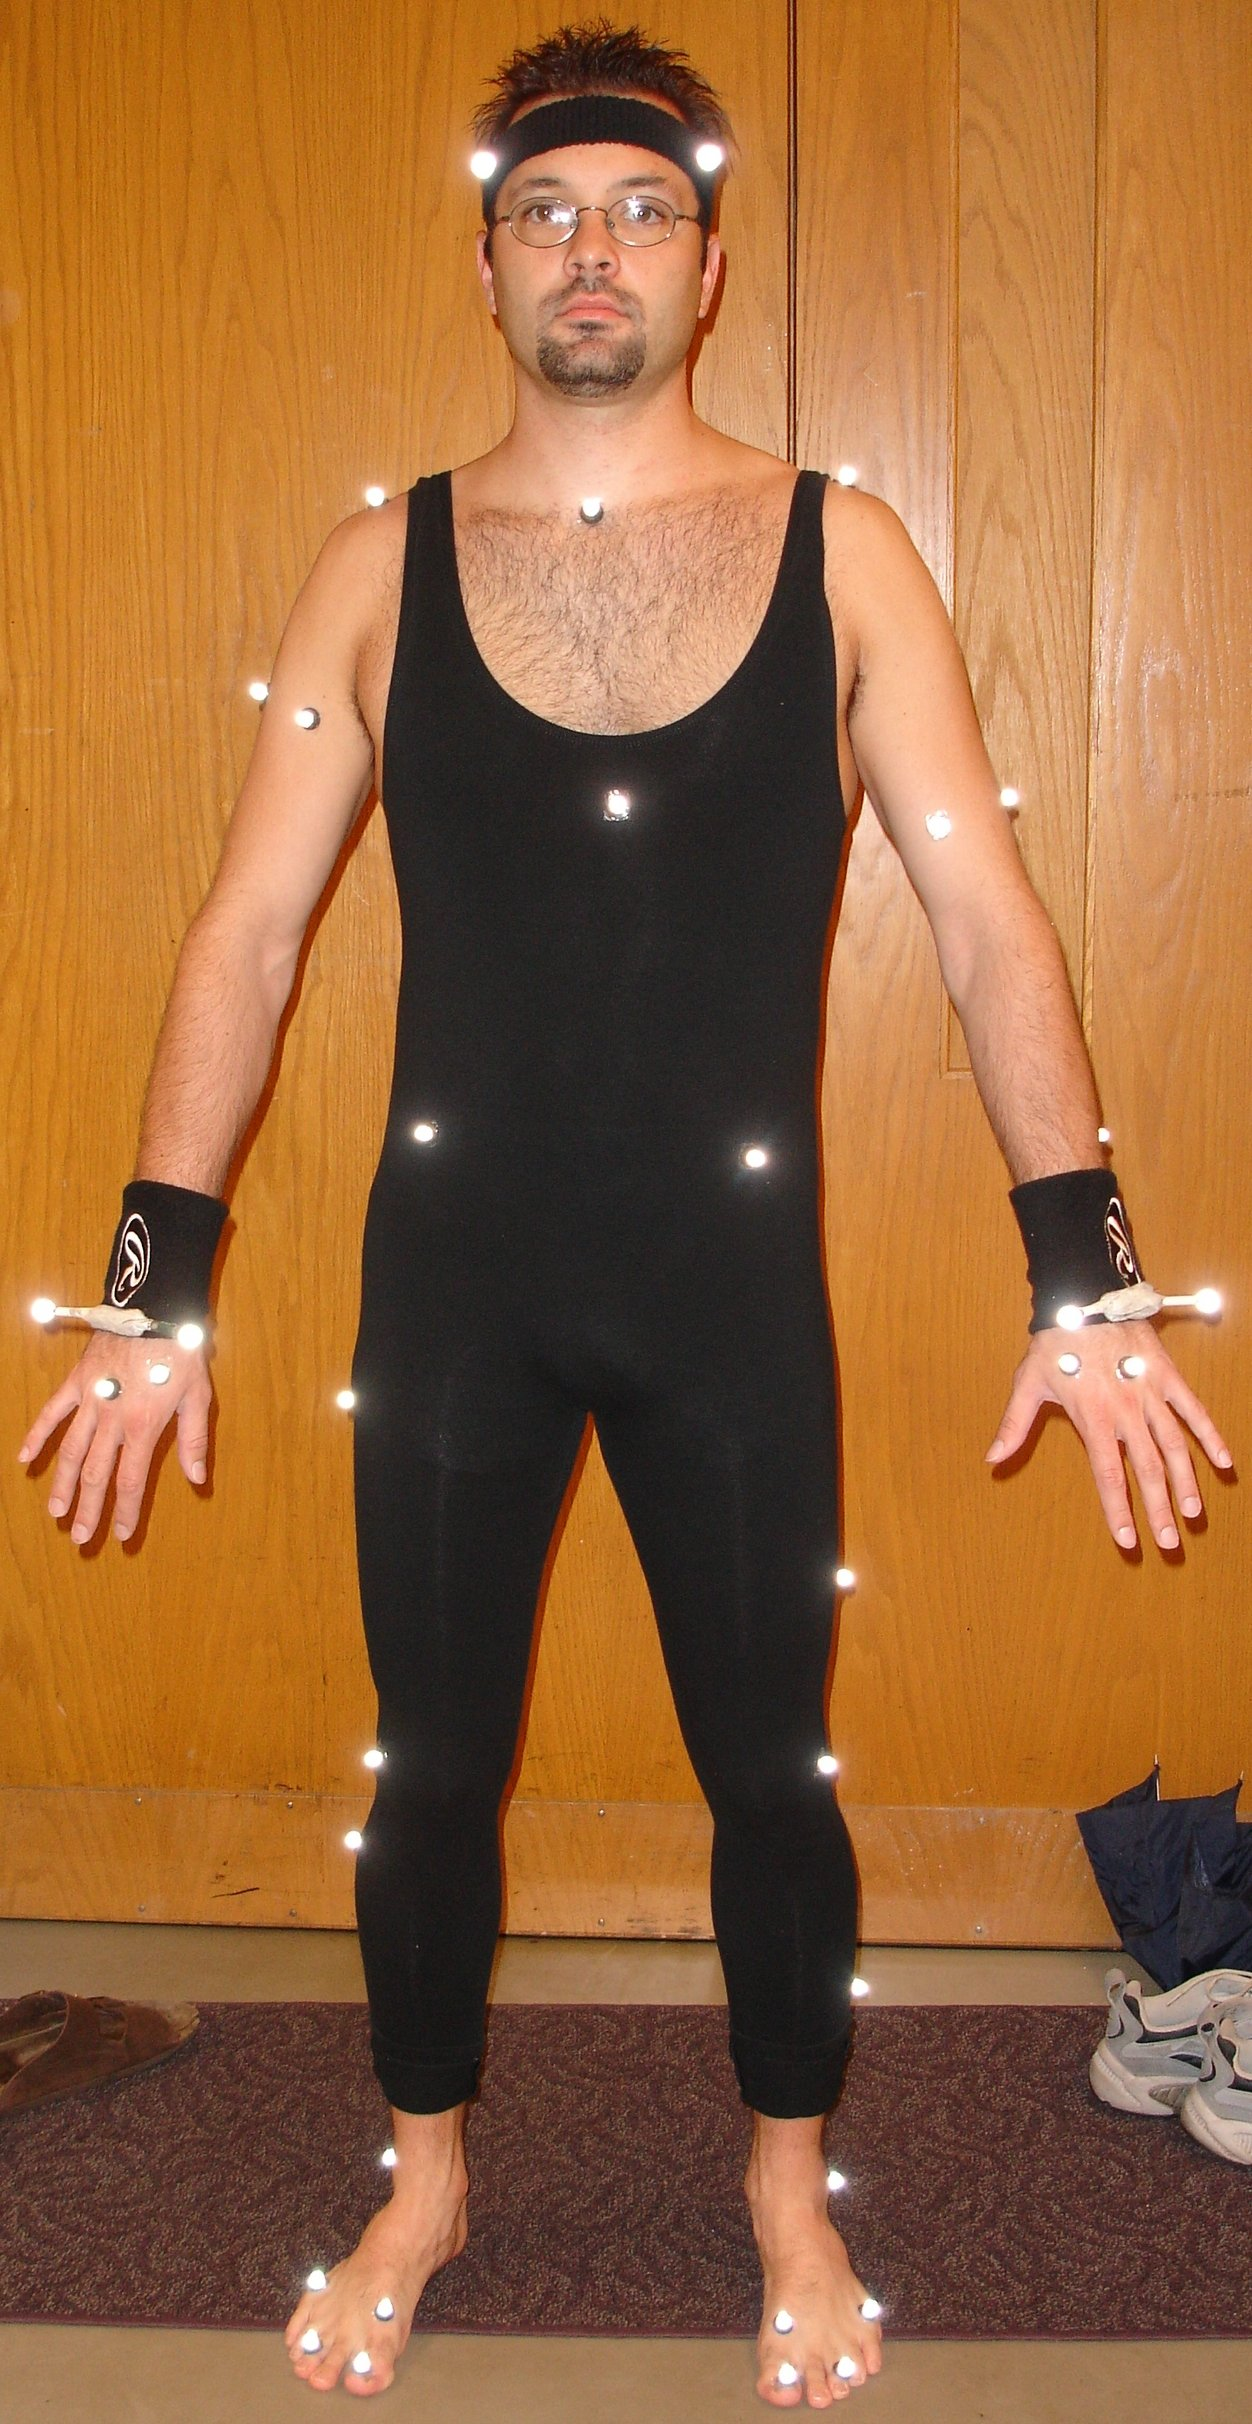
\includegraphics[width=0.3\textwidth]{Imagenes/Bitmap/MCUTraje.jpg}
    \caption{Imágen del traje de captura de movimiento usado para la base de datos de la Universidad Carnegie Mellon, Fuente: https://mocap.cs.cmu.edu/info.php}
    \label{fig:MCUTraje}
\end{figure}

\begin{figure}[H]
    \centering
    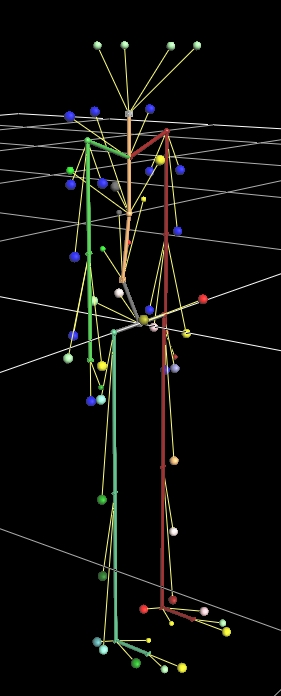
\includegraphics[width=0.23\textwidth]{Imagenes/Bitmap/MCUEsqueleto.jpg}
    \caption{Imágen del esqueleto resultante del traje de captura de movimiento usado por la Universidad Carnegie Mellon, Fuente: https://mocap.cs.cmu.edu/info.php}
    \label{fig:MCUEsqueleto}
\end{figure}

Por otro lado, como ya mencionamos en el capítulo \ref{sec:traje}, el traje Perception Neuron 3 contiene 17 puntos, haciendo incompatibles los esqueletos.

El segundo motivo por el que no se ha usado el dataset de la Universidad Carnegie Mellon es el formato de las animaciones disponibles.
Las animaciones presentes en el dataset vienen en tres formatos distintos: c3d, asf (o amc) y vsk (o v).
Los formatos c3d, vsk y v son unos formatos en binario usados para objetos en 3D, por lo que no se puede usar de forma sencilla para extraer la información del propio archivo.
Por otro lado los archivos asf y amc son archivos en formato ASCII con la información de los huesos. Sin embargo la documentación aportada para poder usar la información es incompleta.

El último motivo por el que no se ha usado este dataset es por la escasez de animaciones de los gestos buscados.
Animaciones como ``correr'' sí están presentes (aunque no en abundancia), pero otras como ``pelear'' o ``saludar'' no.

Este último problema también ha estado presente en páginas específicas de bancos de datasets como Kaggle.

\subsection{Kaggle}

TO DO: HABLAR DE LA ESCASEZ DE DATASET DE ANIMACIONES EN KAGGLE

TO DO: HABLAR DE POR QUÉ DESCARTAMOS IMÁGENES Y NOS CENTRAMOS MÁS EN ESQUELETOS

Ya que no se encontró un gran dataset que cumpliese con nuestros requerimientos se tomó la decisión de buscar en un banco de animaciones los gestos requeridos y transformar esas animaciones en un formato que puediesen ser procesados.
\section{Dataset Artificial}
\label{sec:datasetArtificial}

El banco de animaciones en el que fueron buscados los gestos necesarios fue Mixamo. \footnote{Página web de Mixamo: \url{https://www.mixamo.com}}

Mixamo es una página web creada por Adobe en la que se encuentran de manera gratuita modelos con un \gls{rig} humanoide y animaciones para estos rigs, además de una funcionalidad que permite crear el \gls{rig} de un personaje que se suba a la página.
En la página hay un buscador en el que puedes buscar tipos de animaciones, pero como no es viable descargarse todas las animaciones de todos los gestos buscados se usó una herramienta para automatizarlo.

\subsection{Herramienta para descargarse animaciones de Mixamo de forma automática}

Esta herramienta se encontró en GitHub hecha por el usuario \textit{juanjo4martinez}\footnote{Enlace al perfil del creador de la herramienta \url{https://github.com/juanjo4martinez}}. La herramienta (mixamo-downloader\footnote{Enlace al repositorio de la herramienta \url{https://github.com/juanjo4martinez/mixamo-downloader}}) permite buscar y descargar animaciones de Mixamo de manera automática y con el uso de distintos filtros para acomodarse a lo requerido por el usuario.

Al empezar a usarse la herramienta se detectó que al empezar a bajar animaciones, dependiendo del nombre que tuvieran las mismas, el programa era incapaz de guardar dichas animaciones. Esto se debía a la incompatibilidad de distintos sistemas de archivos para usar determinados caracteres en sus nombres de archivos (interrogaciones, barras o dobles barras, dos puntos, etc). Se hizo un \gls{fork} de la herramienta \footnote{Enlace al repositorio con los arreglos \url{https://github.com/ALK222/mixamo-downloader}} que efectúa estos arreglos y añade la opción de reescribir animaciones anteriores que tuvieran el mismo nombre. La interfaz completa de la herramienta arreglada se puede ver en la figura \ref{fig:mixamo-downloader}.

\begin{figure}[H]
    \centering
    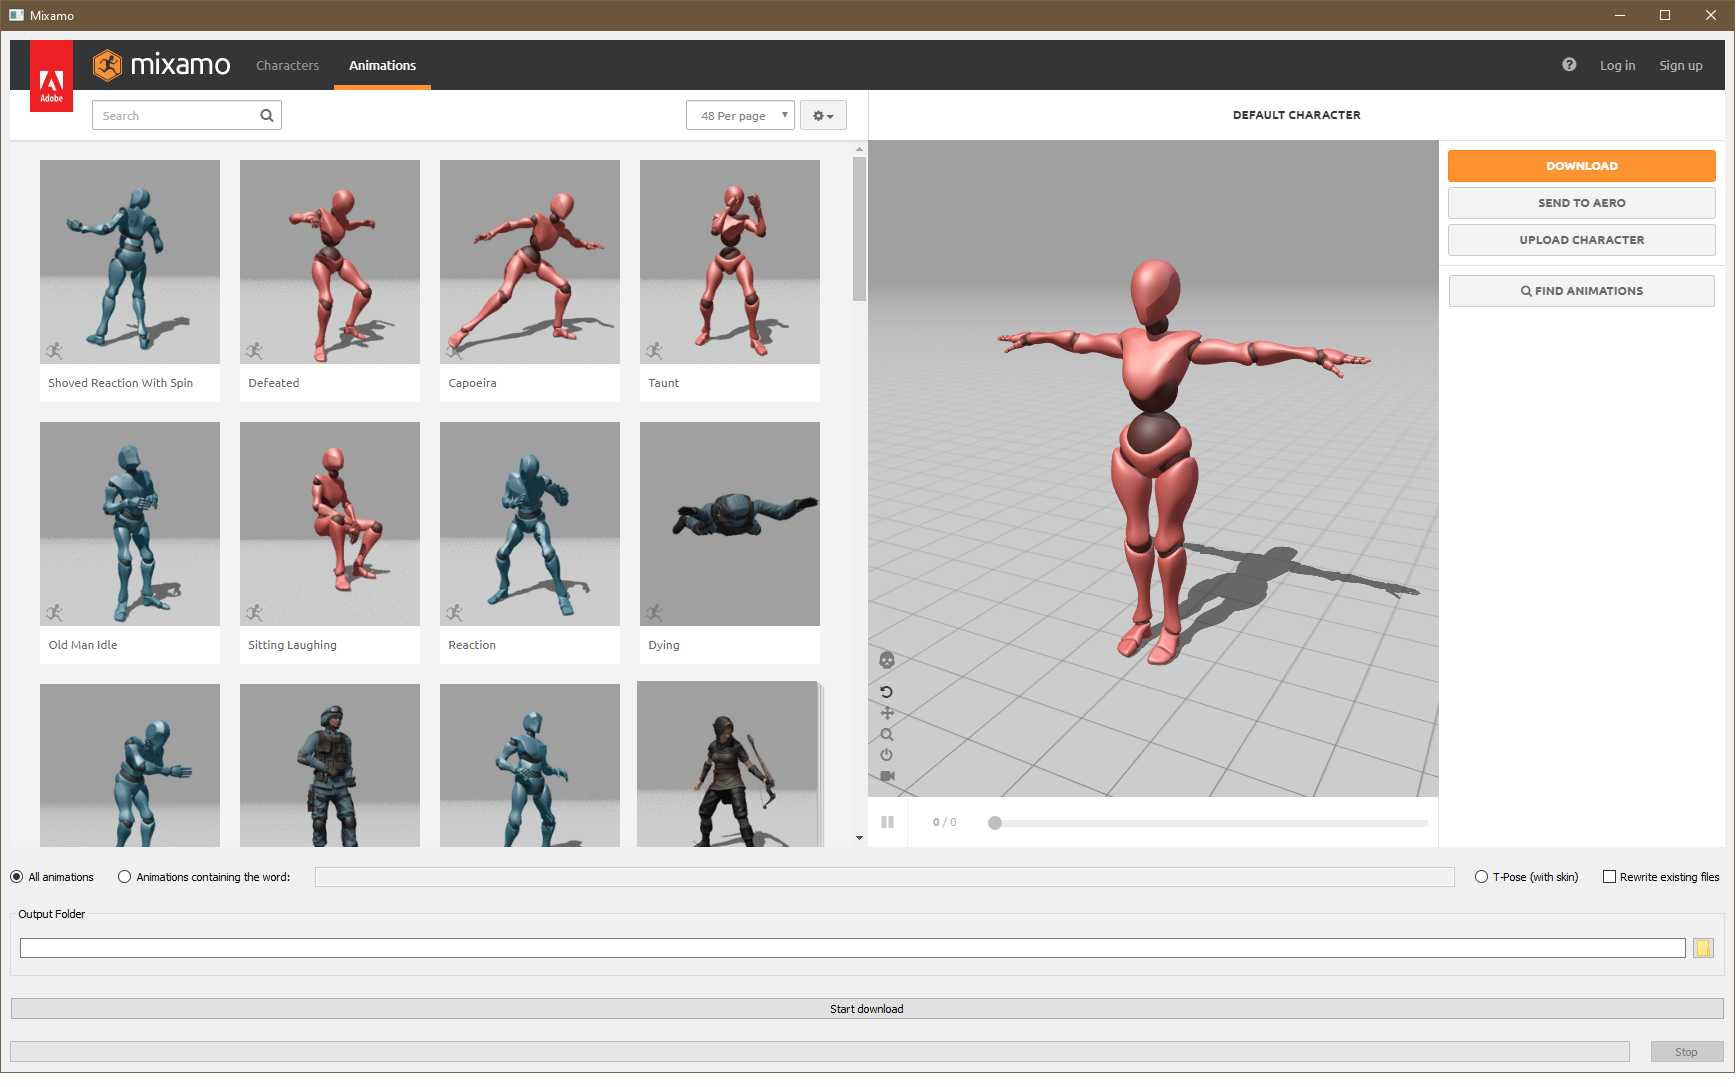
\includegraphics[width=0.7\textwidth]{Imagenes/Bitmap/caputra-mixamo-downloader.png}
    \caption{Herramienta Mixamo Downloader Arreglada}
    \label{fig:mixamo-downloader}
\end{figure}

Una vez realizados los cambios, se descargaron las animaciones disponibles en Mixamo para los gestos que se querían usar. El resultado de estas descargas se puede ver en el dataset \cite{raw-mixamo-animations}.

Las animaciones descargadas tienen un formato \gls{FBX}, por lo que era necesario pasarlas a un formato que puedan usar los modelos de \gls{ia}.
Para ello se decidió pasar la información relevante de los huesos en la toda la animación (su posición y rotación en cada frame) a un archivo CSV, donde cada columna iba a ser esta información y cada fila un frame de la animación. En la tabla \ref{tab:cabecera-csv-completa} se puede ver la cabecera para los CSV. En la siguiente tabla (\ref{tab:cabecera-csv-incompleta}) se puede ver un ejemplo de los valores que se guardan de un punto concreto del traje.

\begin{longtblr}[
        caption={Cabecera del \gls{csv} de cada animación, en órden descendente y de izquierda a derecha (incompleta).},
        label={tab:cabecera-csv-incompleta}
    ]{
        colspec={|l|l|l|},
        rowhead=1,
        hlines,
        row{even}={gray9},
        cells   = {font=\footnotesize\linespread{0.84}\selectfont},
    }
    Robot\_Hips\_posx &
    Robot\_Hips\_posy &
    Robot\_Hips\_posz   \\
    Robot\_Hips\_rotx &
    Robot\_Hips\_roty &
    Robot\_Hips\_rotz   \\
    ...               &
    ...               &
    ...                 \\
\end{longtblr}

Como no es viable ni escalable meter todas las animaciones a un proyecto de Unity ni crear un \gls{Animator} con todas estas se ideó una herramienta en Unity que se metiese todas las animaciones y construía el Animator en tiempo de ejecución.

\subsection{Carga mediante asset bundles}
En un principio se pensó en usar los assets bundles para cargar las animaciones.
Los assets bundles son archivos de Unity que contienen archivos serializados (cualquier asset para un videojuego menos código) y pueden cargarse en tiempo de ejecución.
Finalmente se descartó la idea de usar este tipo de archivos, ya que necesitan construirse en un proyecto de Unity, por lo que no solucionaba el problema de meter las animaciones a mano a un proyecto de Unity

\subsection{Carga mediante Asset Database}
Finalmente se decidió usar Asset Database para la carga automática de las animaciones.
Asset Database es una API de Unity que permiten trabajar con assets, siempre y cuando estén incluidos en el proyecto aunque no necesariamente cargados.
Para suplir la condición de que estuviesen incluidos en el proyecto se hizo un script que descargaba las animaciones, separadas por carpetas cuyo nombre era el tipo de gesto, desde la base de datos de Kaggle hacia la carpeta ``Resources'' del proyecto y ejecutaba desde línea de comandos el editor del proyecto.

Una vez las animaciones estuviesen descargadas en la carpeta de ``Resources'' del proyecto se busca iterativamente por la carpeta para cargar las animaciones y guardarse la relación entre el tipo de gesto y la animación.
Una vez completado empieza la ejecución de las animaciones.

Esta ejecución consiste en cargar la animación en la máquina de estados del \gls{Animator} gracias a un componente llamado ``Animator Override Controller'', que permite cambiar el clip de animación de una instancia del \gls{Animator} sin cambiar la lógica de su máquina de estados.
Cuando empieza la animación se crea un \gls{csv} con el formato ``Animación\_Número de animación.csv'' y empieza su ejecución.
Una vez finalizada la ejecución de una animación se cierra el \gls{csv} y se busca la siguiente animación. Se puede ver un ejemplo de todo este proceso en un timelapse de la ejecución de la herramienta\footnote{Enlace al timelapse completo a x4 de tiempo \url{https://youtu.be/NOawMoaG98M}}, también se deja una captura del mismo para ver el funcionamiento de la herramienta en el editor de Unity en la figura \ref{fig:frame-timelapse}, donde se puede ver al avatar ``Remy'' en mitad de una animación de baile. Este avatar lleva a cabo las animaciones del dataset para, en cada frame de ejecución, convertir sus coordenadas al \gls{csv} correspondiente.

\begin{figure}[H]
    \centering
    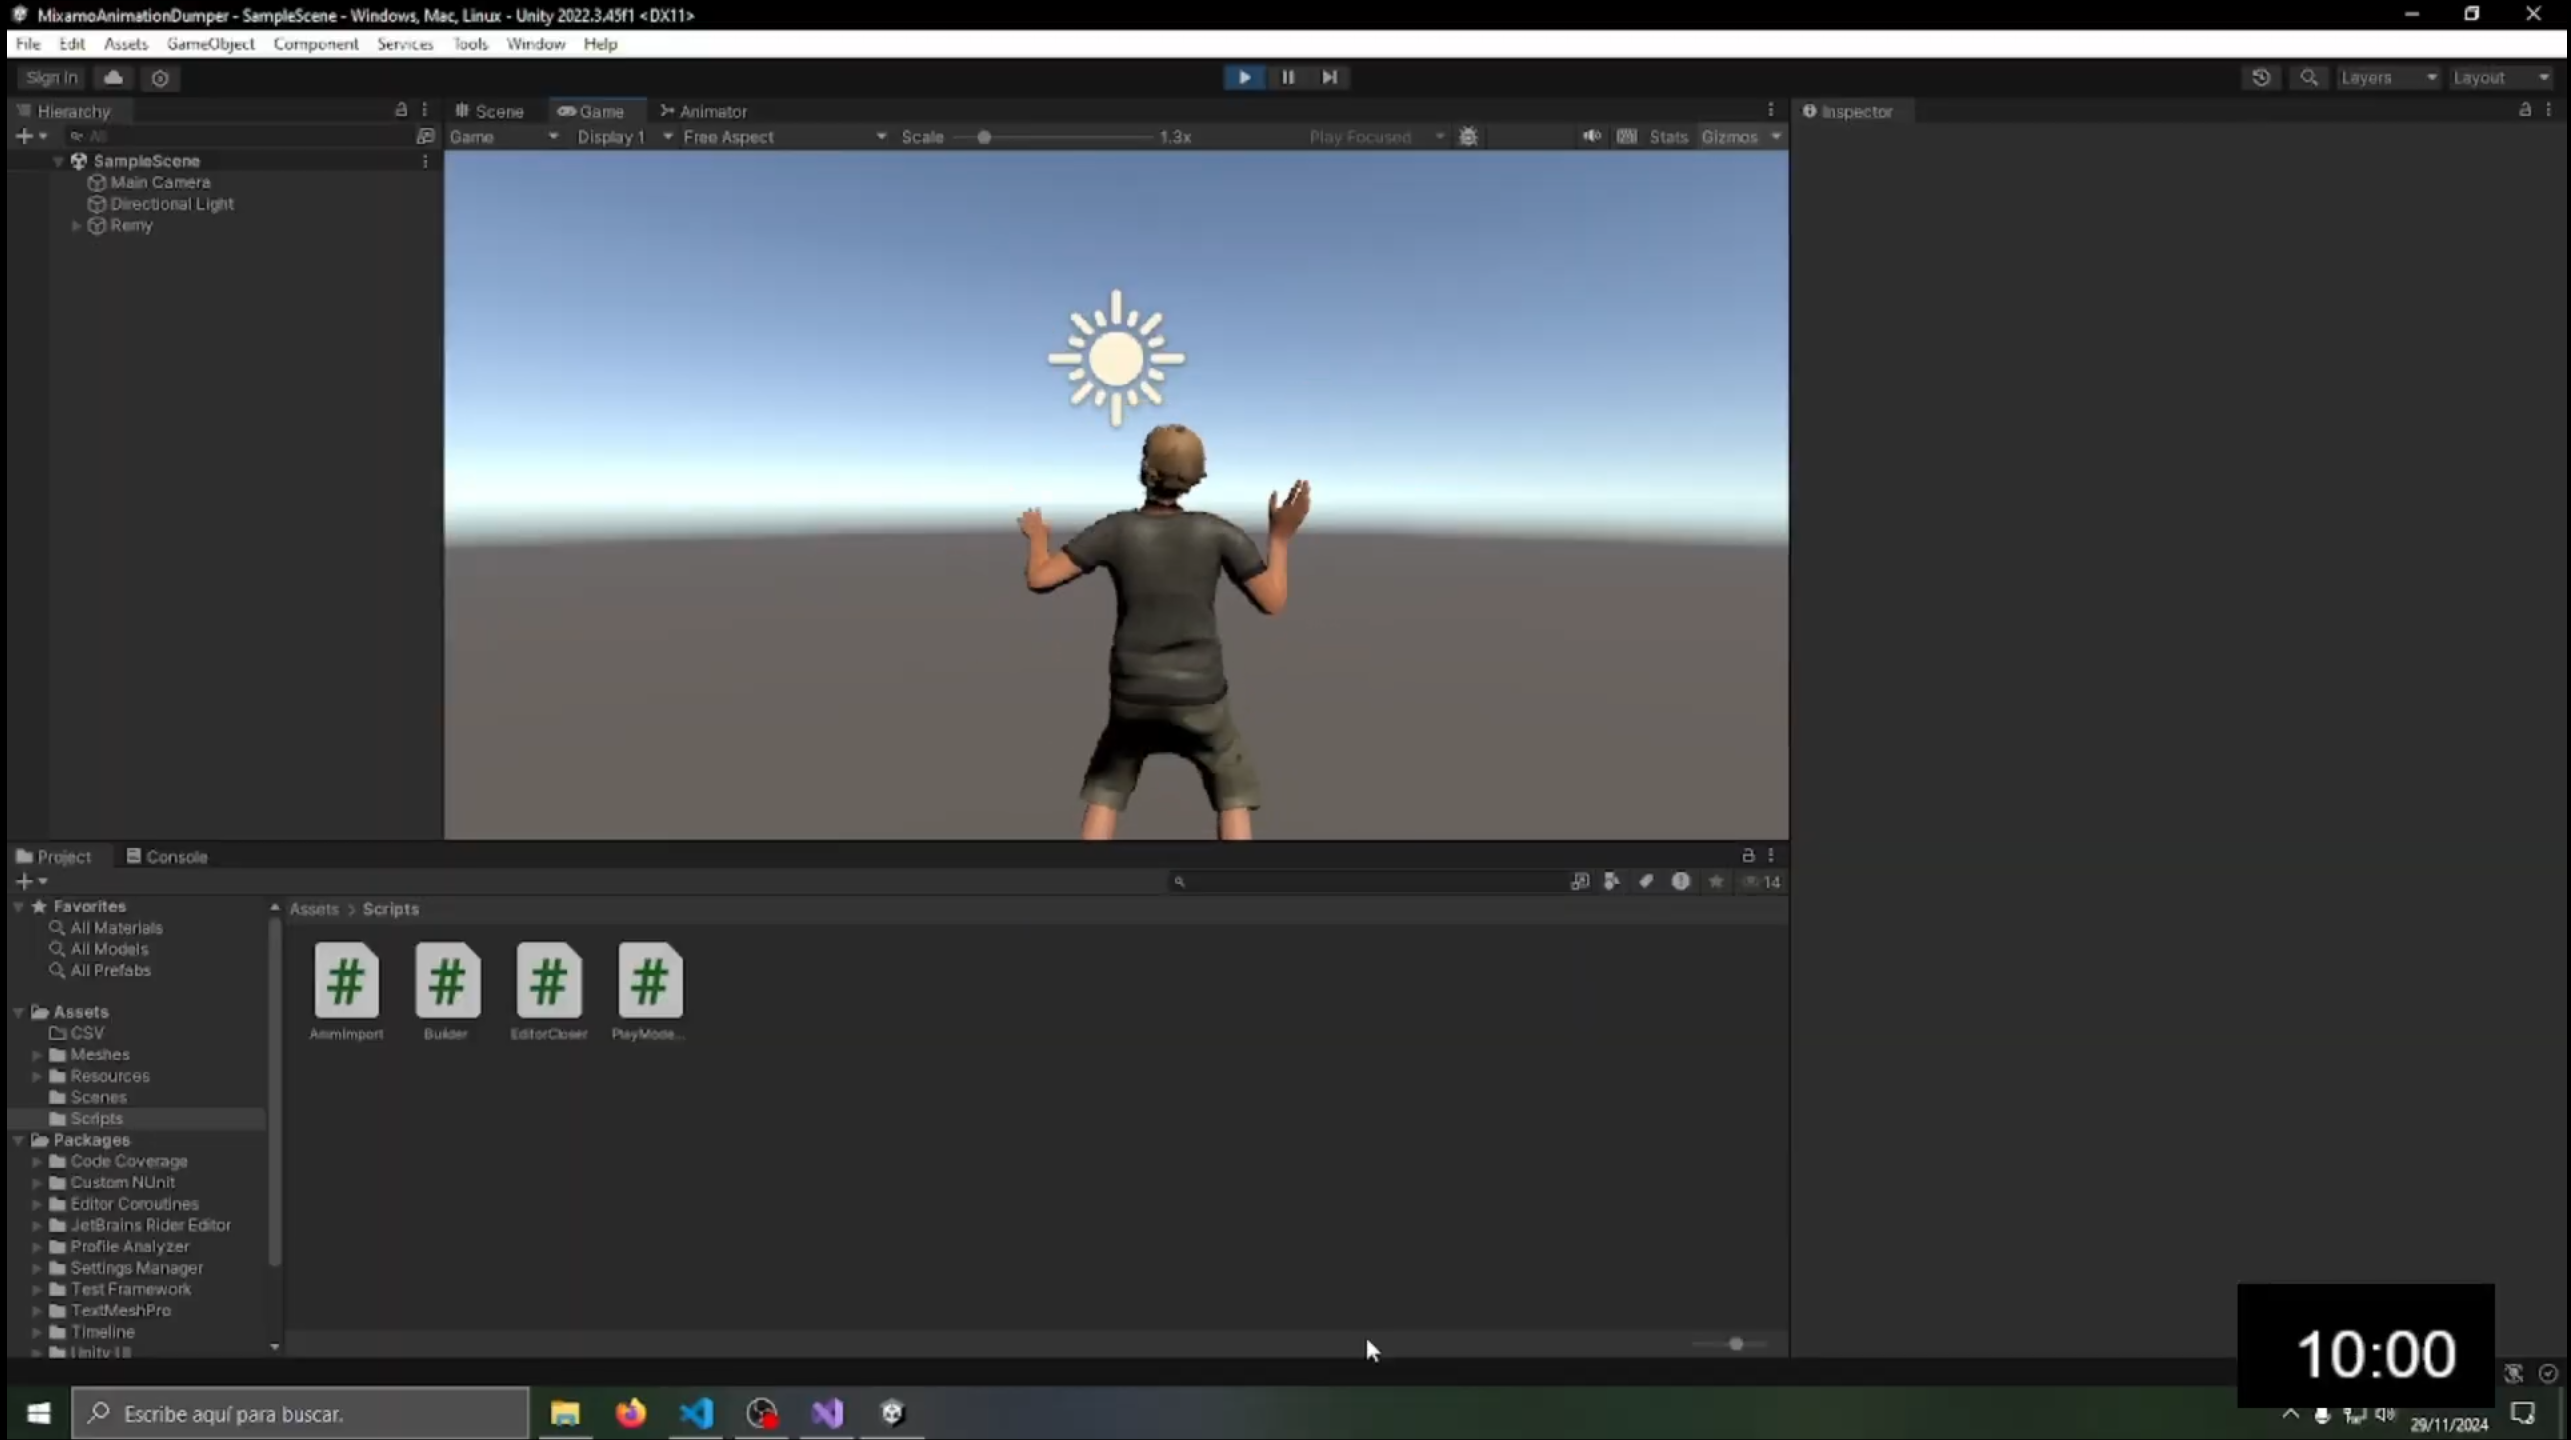
\includegraphics[width=0.7\textwidth]{Imagenes/Bitmap/remy_bailon.png}
    \caption{Frame de un \textit{timelapse} de la ejecución de la herramienta}
    \label{fig:frame-timelapse}
\end{figure}

En la figura \ref{fig:MixamoDumper} se puede ver un diagrama de flujo del funcionamiento de esta herramienta, mientras que el código de la misma es público\footnote{Enlace al repositorio de la herramienta: \url{https://github.com/FratosVR/Mixamo-Animation-Dumper}} y se puede ver en el apéndice \ref{appendix:MixamoDumperCode}.

\newpage

\begin{figure}[H]
    \centering
    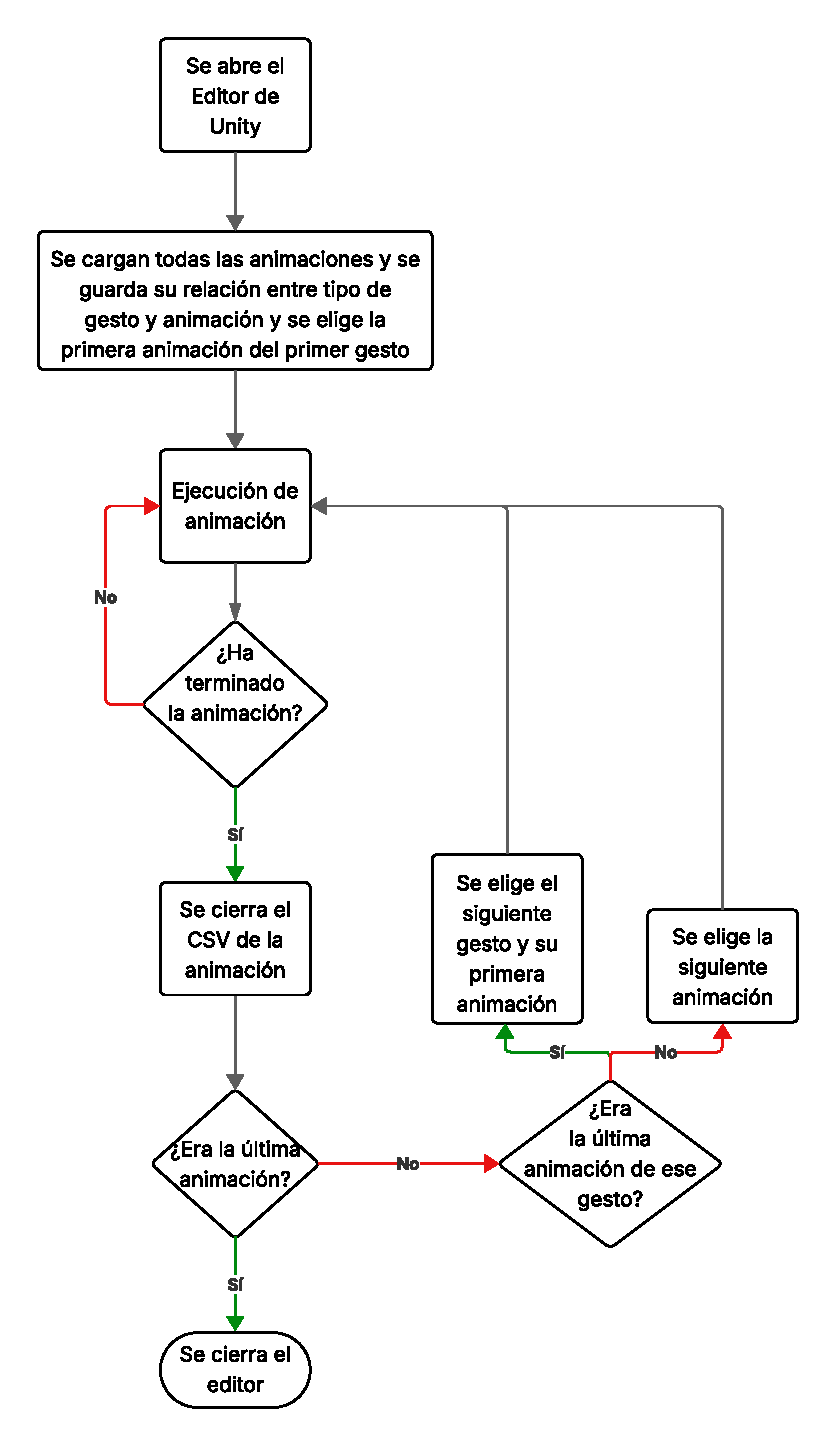
\includegraphics[width=0.7\textwidth]{Imagenes/Vectorial/FlujoMixamoDumper.pdf}
    \caption{Diagrama de flujo de la herramienta que carga y ejecuta las animaciones de Mixamo en tiempo de ejecución, llamada Mixamo Dumper}
    \label{fig:MixamoDumper}
\end{figure}

El número de annimaciones que se consiguieron grabar se puede ver en la figura \ref{fig:AnimacionesBruto}, donde se puede observar un desbalanceo de algunas animaciones (bailar o pelear) frente a otras (saludar o señalar).

\begin{figure}[H]
    \centering
    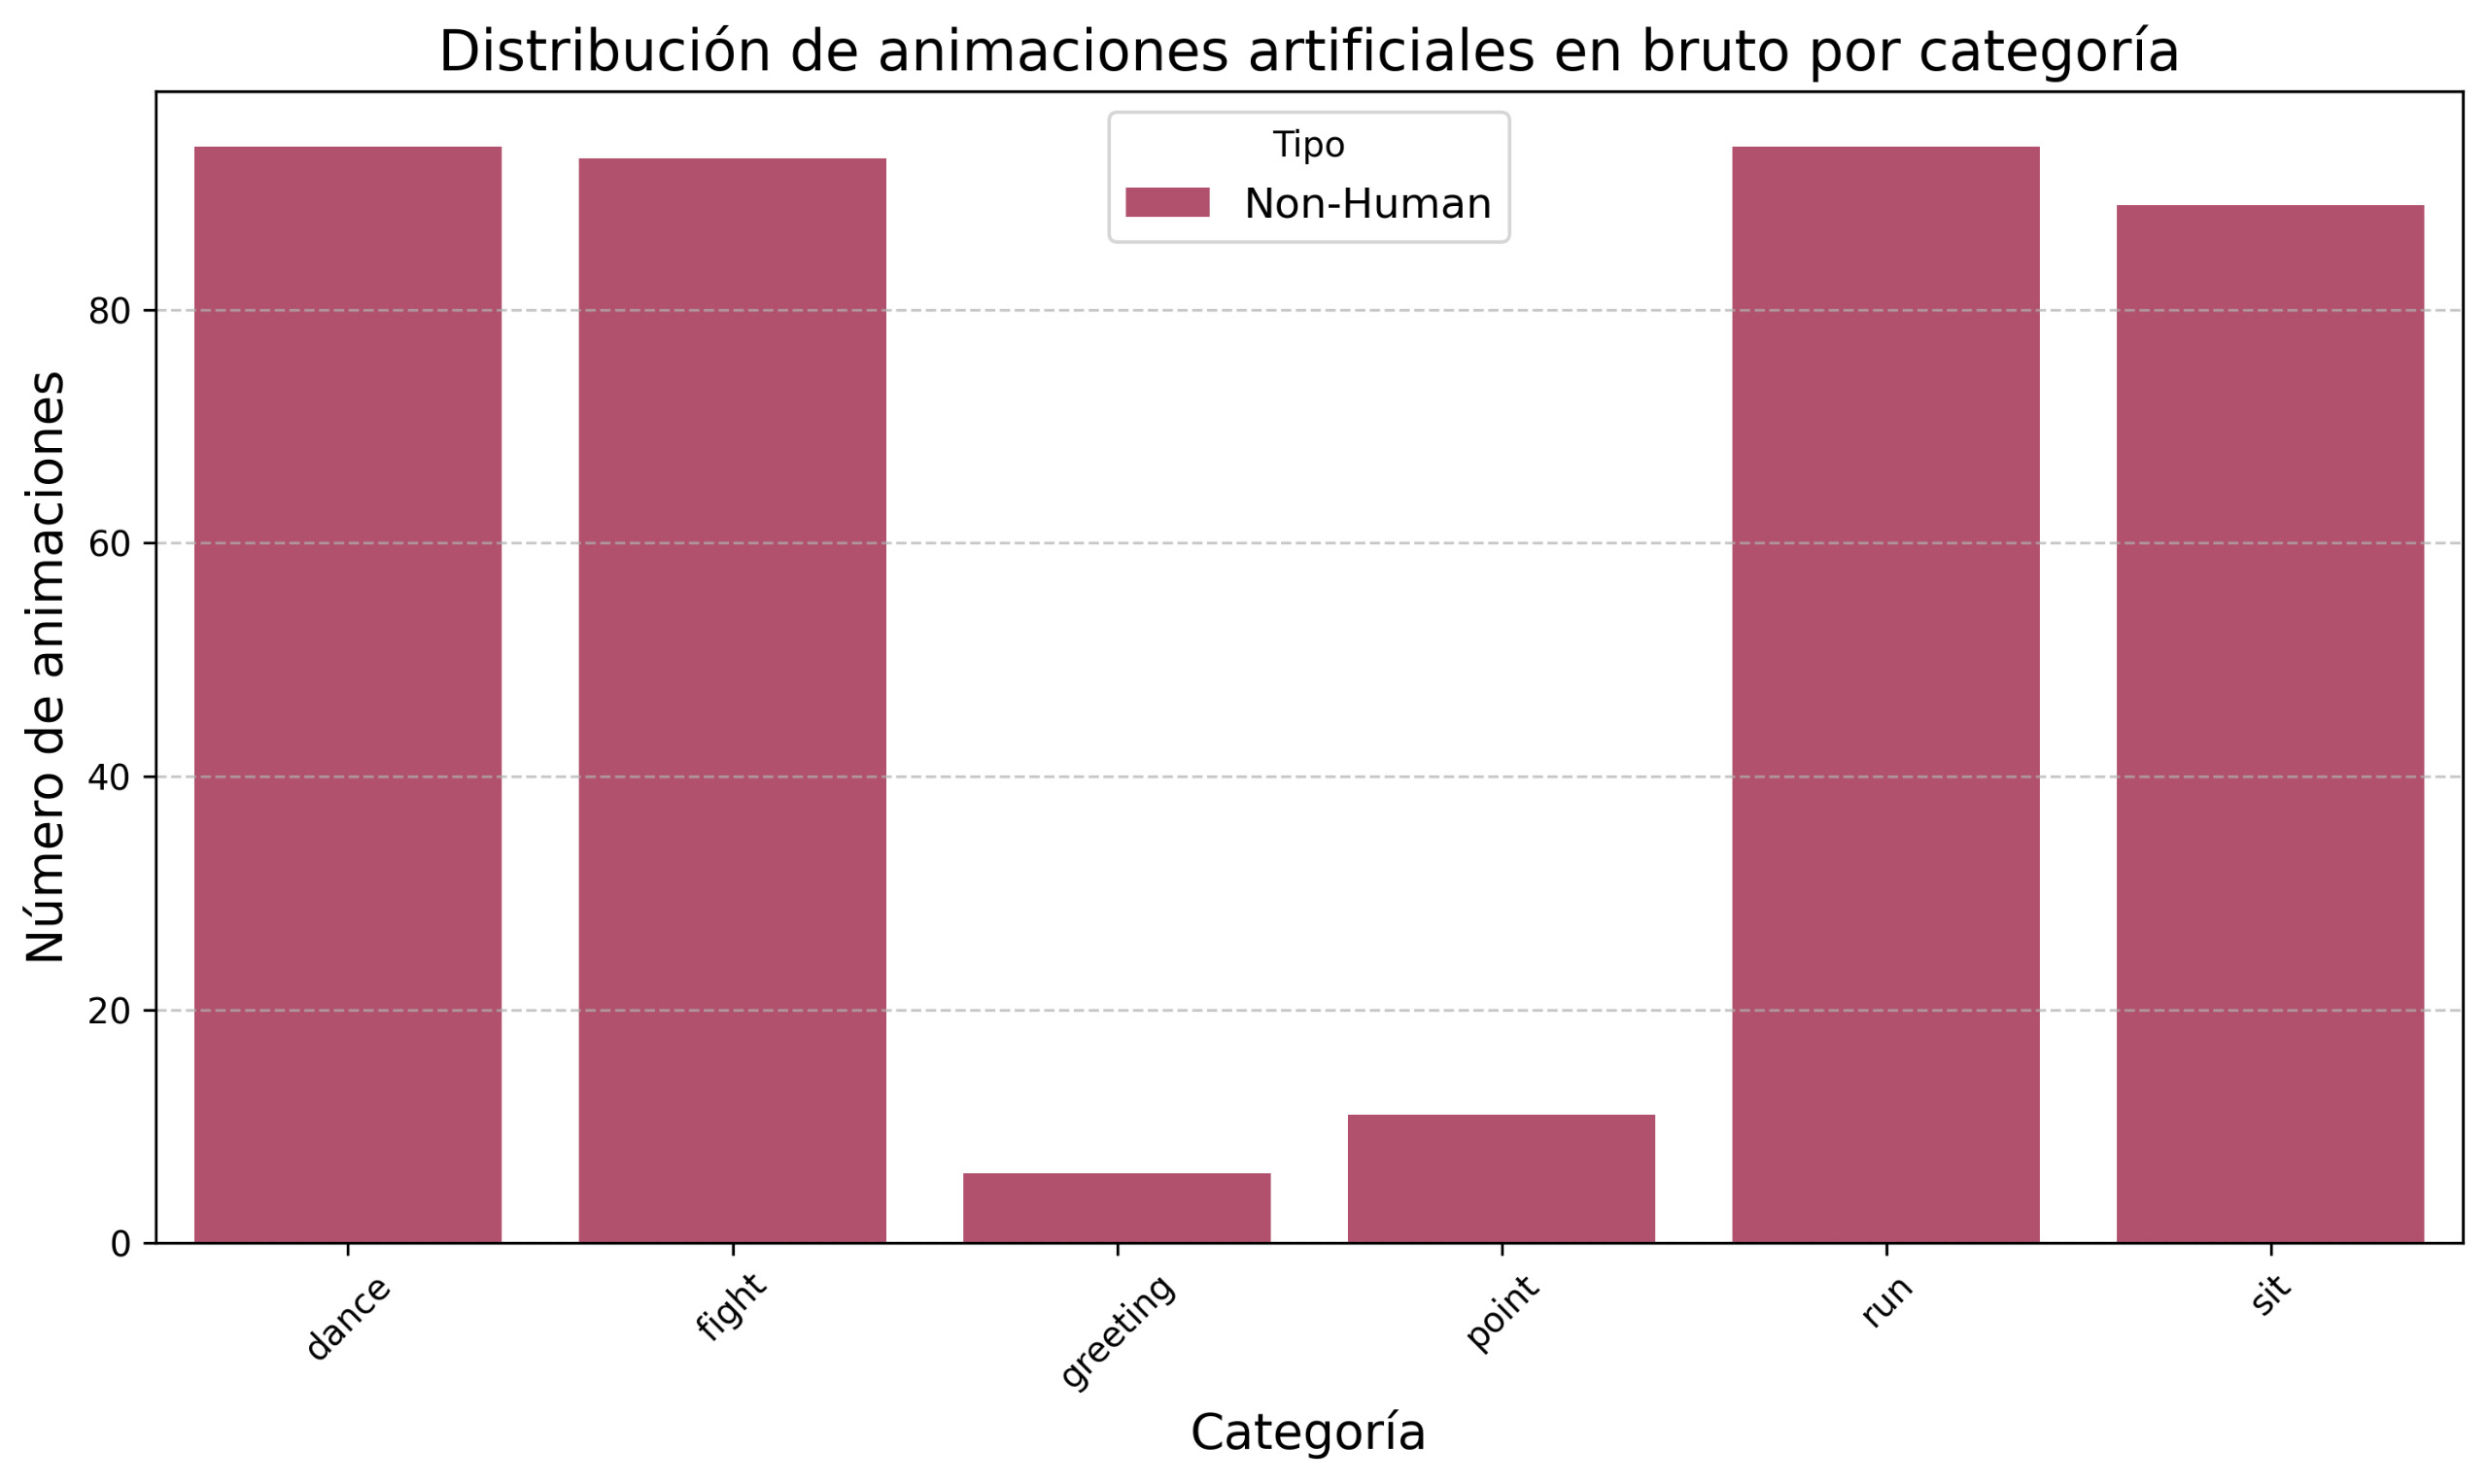
\includegraphics[width=0.8\textwidth]{Imagenes/Bitmap/AnimacionesBruto.jpeg}
    \caption{Número de animaciones conseguidas gracias a la herramienta divididas por tipo de gesto}
    \label{fig:AnimacionesBruto}
\end{figure}

Al finalizar todas las animaciones se cierra el editor de Unity y se procesan los CSV resultantes.

La ventaja de hacer esta herramienta es que es independiente del número de gestos y de animaciones por cada gesto, lo que hace que esta herramienta haga escalable el caso de que se quieran introducir o quitar gestos.

\subsection{Tratamiento de CSV resultantes}

Los \glspl{csv} restantes se copiaron en un nuevo \textit{dataset} de Kaggle en una carpeta llamada ``full\_animations''. Una vez subidos estos datos, se creó una clase en Python para estandarizar estos \glspl{csv}. Los datos se estandarizaron con el siguiente criterio:
\begin{itemize}
    \item Todas las animaciones deben de tener el mismo número de frames. Para ello se estandarizará la duración a 90 frames que es el número de \gls{fps} que usan las gafas de \gls{vr} de Meta Quest 2 y la herramienta Mixamo Animation Dumper.
    \item Las animaciones que duraran más de 90 frames se dividen en varias animaciones de 90 frames o menos.
    \item Las animaciones que duraran menos de 90 frames se repiten desde el inicio hasta completar los 90 frames.
    \item Las animaciones que no lleguen a 10 frames se consideran inválidas y se eliminan.
\end{itemize}

Este proceso se puede ver de manera más visual en la figura \ref{fig:data_cleaner} y se puede ver el diagrama de la clase DataLoader \footnote{Enlace de la herramienta \url{https://github.com/FratosVR/Models/src/DataLoader.py}} en la figura \ref{fig:data_loader}, algunas de las funciones de esta clase se verán en los próximos apartados.

\begin{figure}[H]
    \centering
    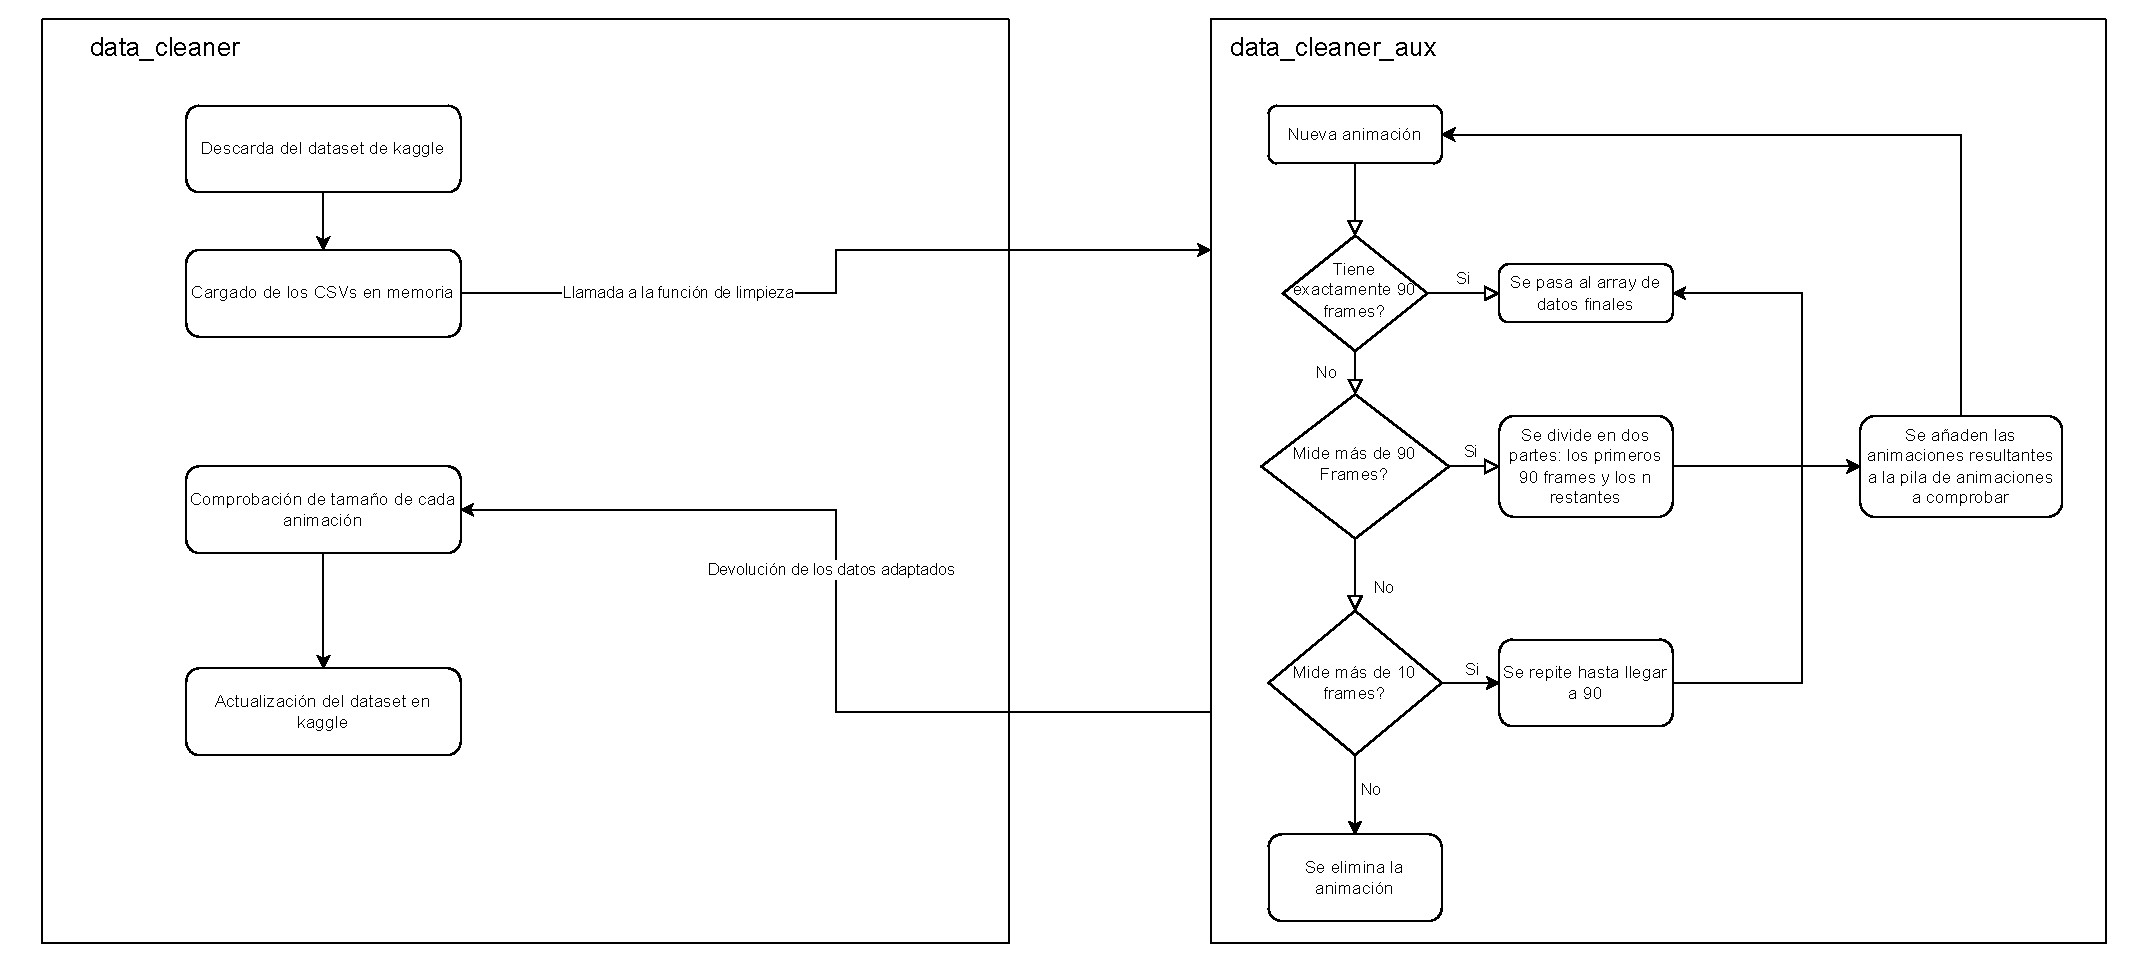
\includegraphics[width=0.8\textwidth]{Imagenes/Vectorial/data_cleaner.pdf}
    \caption{Diagrama de flujo del proceso de limpieza de datos (funciones data\_cleaner y data\_cleaner\_aux de la clase DataLoader)}
    \label{fig:data_cleaner}
\end{figure}

\begin{figure}[H]
    \centering
    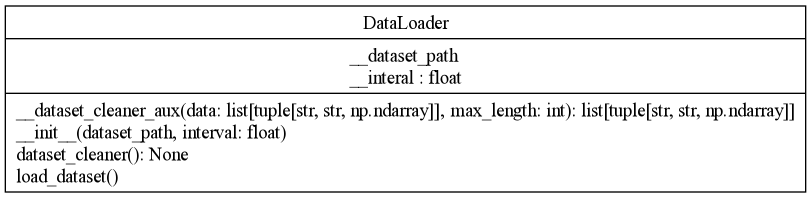
\includegraphics[width=0.9\textwidth]{Imagenes/Bitmap/DataLoader_UML.png}
    \caption{Diagrama de la clase DataLoader}
    \label{fig:data_loader}
\end{figure}

El resultado de la estandarización se puede ver en la figura \ref{fig:AnimacionesEstandar}, donde se puede ver una diferencia notable entre las animaciones de bailar frente al resto.

\begin{figure}[H]
    \centering
    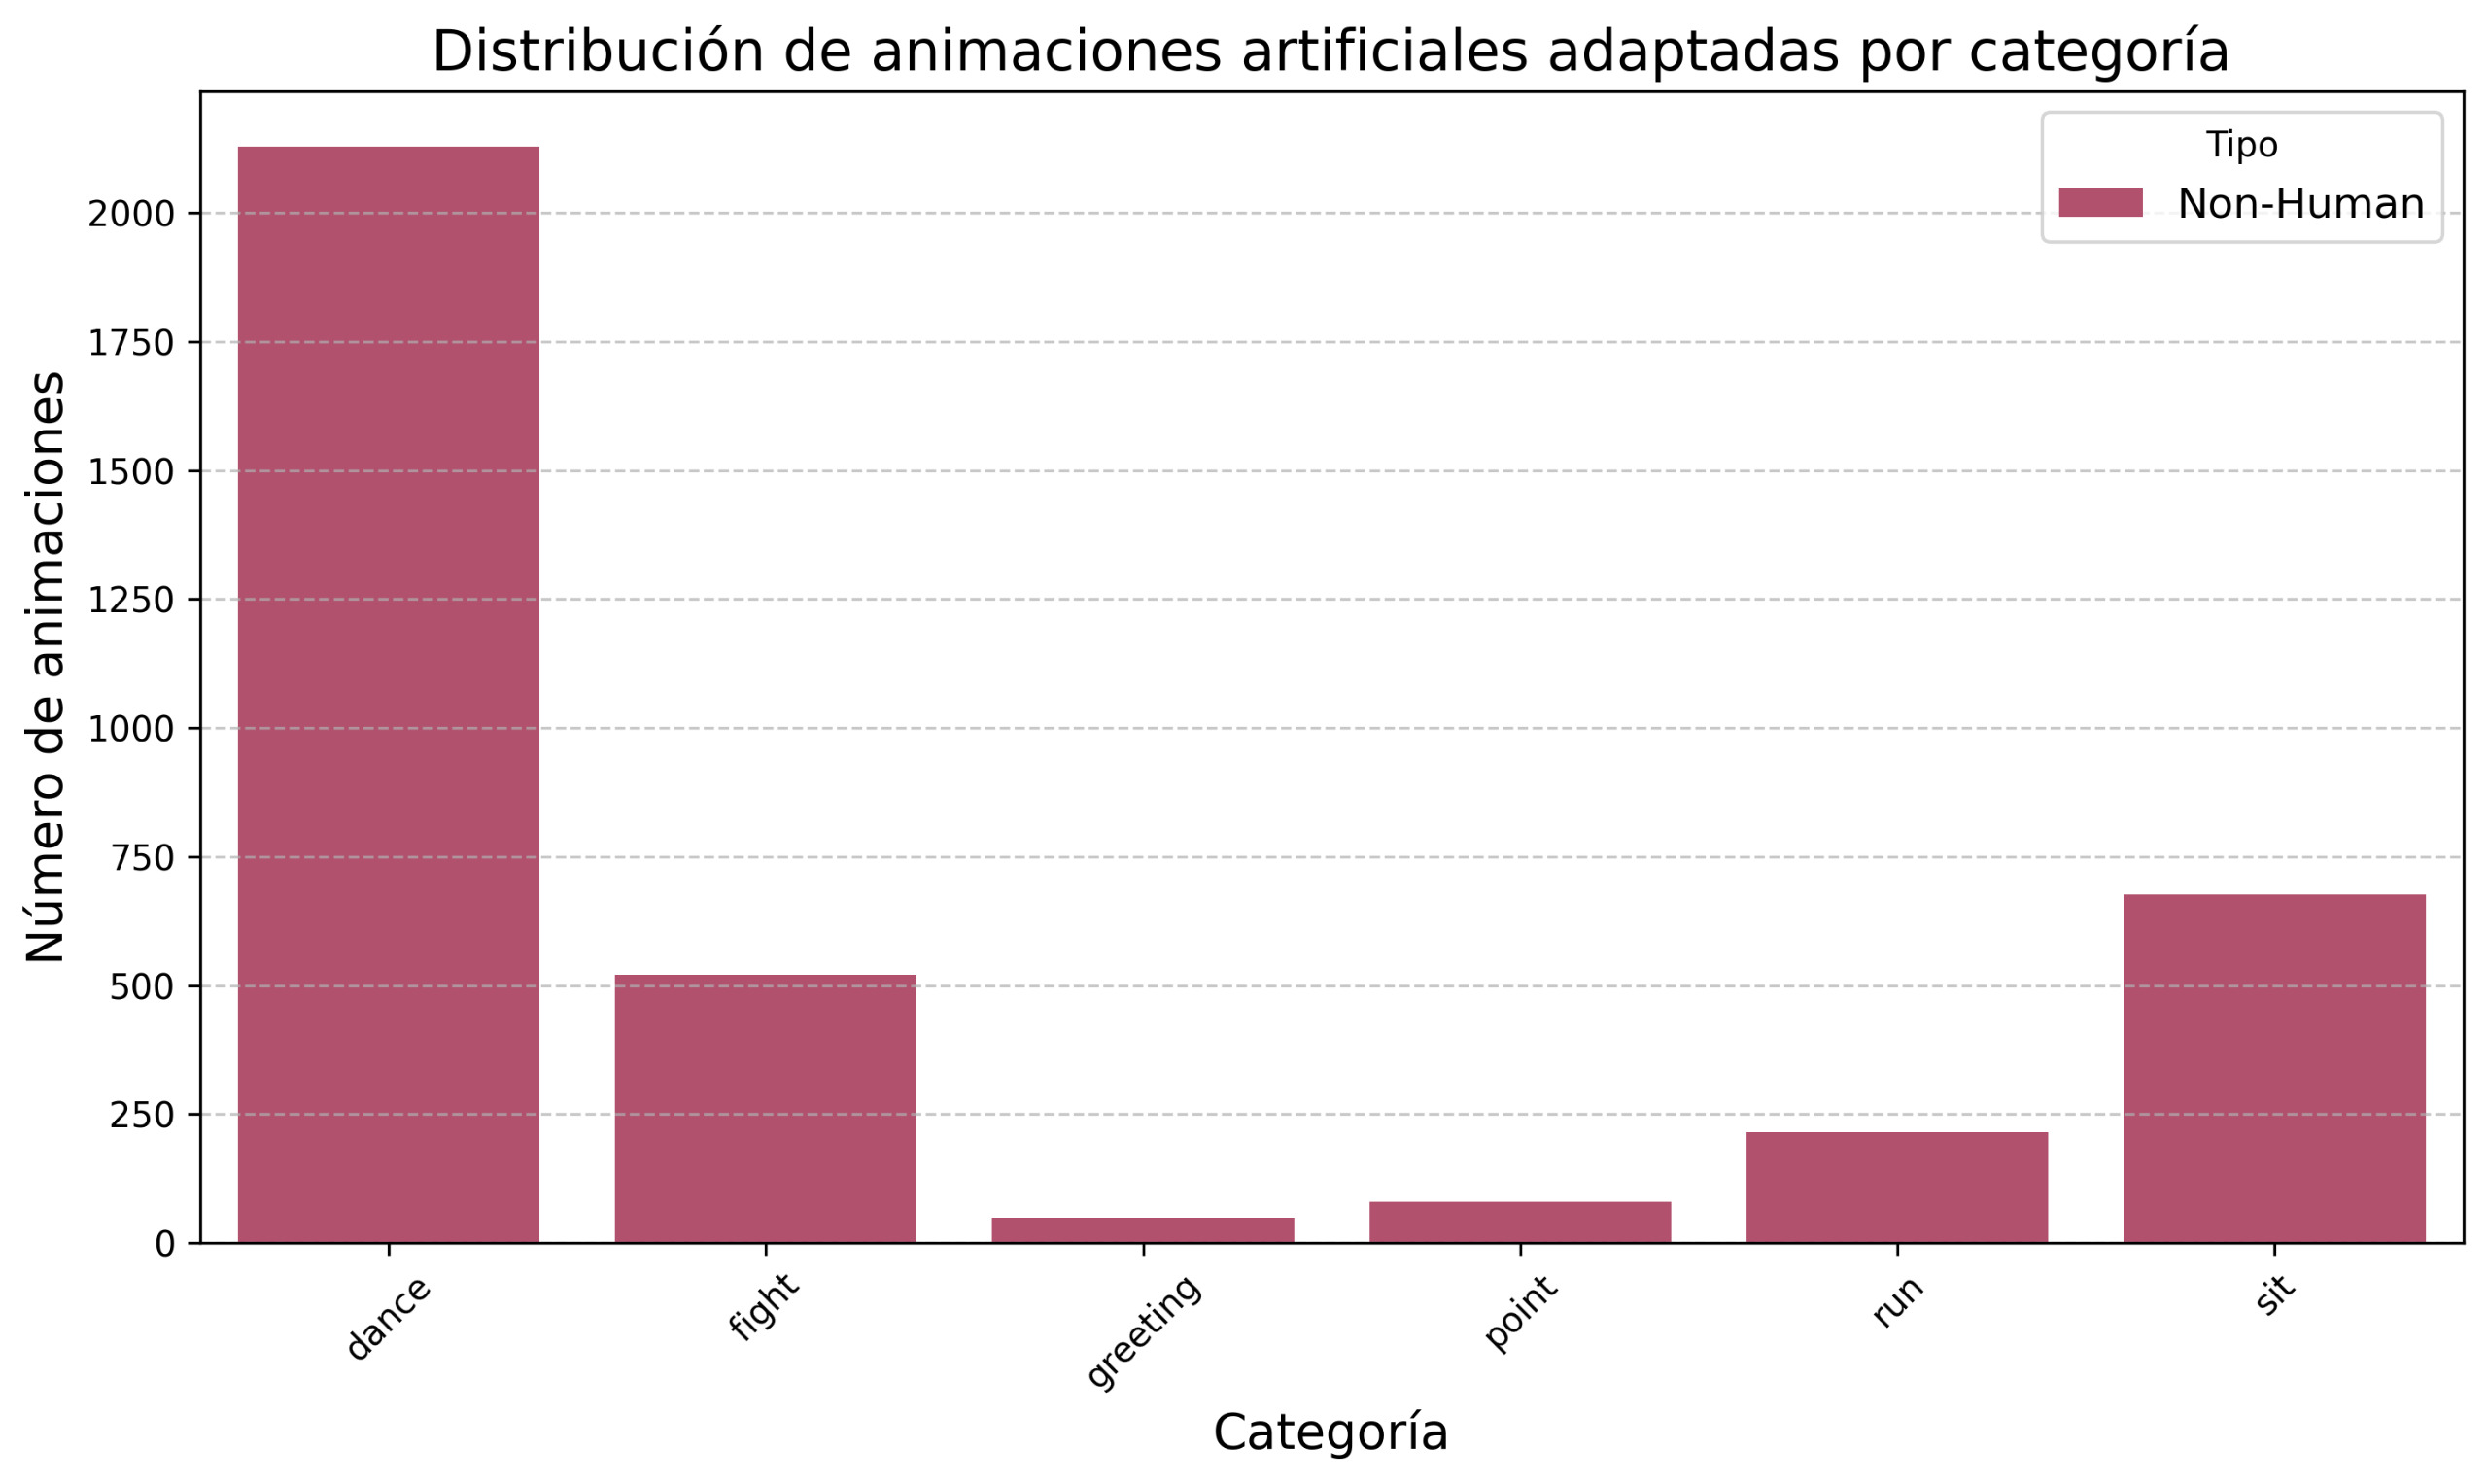
\includegraphics[width=0.8\textwidth]{Imagenes/Bitmap/AnimacionesEstandarizadas.jpeg}
    \caption{Número de animaciones estandarizadas divididas por tipo de gesto}
    \label{fig:AnimacionesEstandar}
\end{figure}

\section{Dataset real}
\label{sec:datasetReal}
Debido a que las animaciones encontradas en el banco de animaciones no eran las suficientes y estaban descompensadas se decidió crear una herramienta para poder recoger los datos de usuarios.

\subsection{Traje}
\label{sec:traje}

Para poder recoger el movimiento de los usuarios era necesario configurar el traje y poder usarlo dentro de Unity.
El traje usado, Preception Neuron 3, viene con:

\begin{enumerate}
	\renewcommand{\theenumi}{\alph{enumi}}
	\item 17 sensores identificados con cada punto.
	\item 15 Bandas de velcro que se ponen en el cuerpo para colocar los sensores.
	\item 3 puertos de carga para los sensores junto a 3 cables USB-C para conectarlos.
	\item 1 USB que contiene la licencia para poder conectar el traje al ordenador.
	\item 1 USB-C que funciona de receptor de las señales del traje.
\end{enumerate}

Para poder usar el traje se necesita la aplicación Axis Studio. \footnote{Enlace a la página de descarga de Axis Studio: \url{https://www.noitom.com/perception-neuron-downloads}}
\subsubsection{Axis Studio y conexión del traje}
Axis Studio es la aplicación creada por Noitom para poder capturar y grabar el movimiento en tiempo real y transmitirlo a aplicaciones de terceros (Unity, Blender o Unreal por ejemplo).

Mientras la aplicación está abierta es necesario tener el USB de la licencia introducido en el equipo.
Al abrir la aplicación y crear un proyecto aparece un espacio vacío (como se puede ver en la figura \ref{fig:AxisSinTraje}) en la parte izquierda de la pantalla, que es donde se verá en tiempo real la captación de movimiento; y un panel de la información del traje en la parte derecha.

\begin{figure}[H]
	\centering
	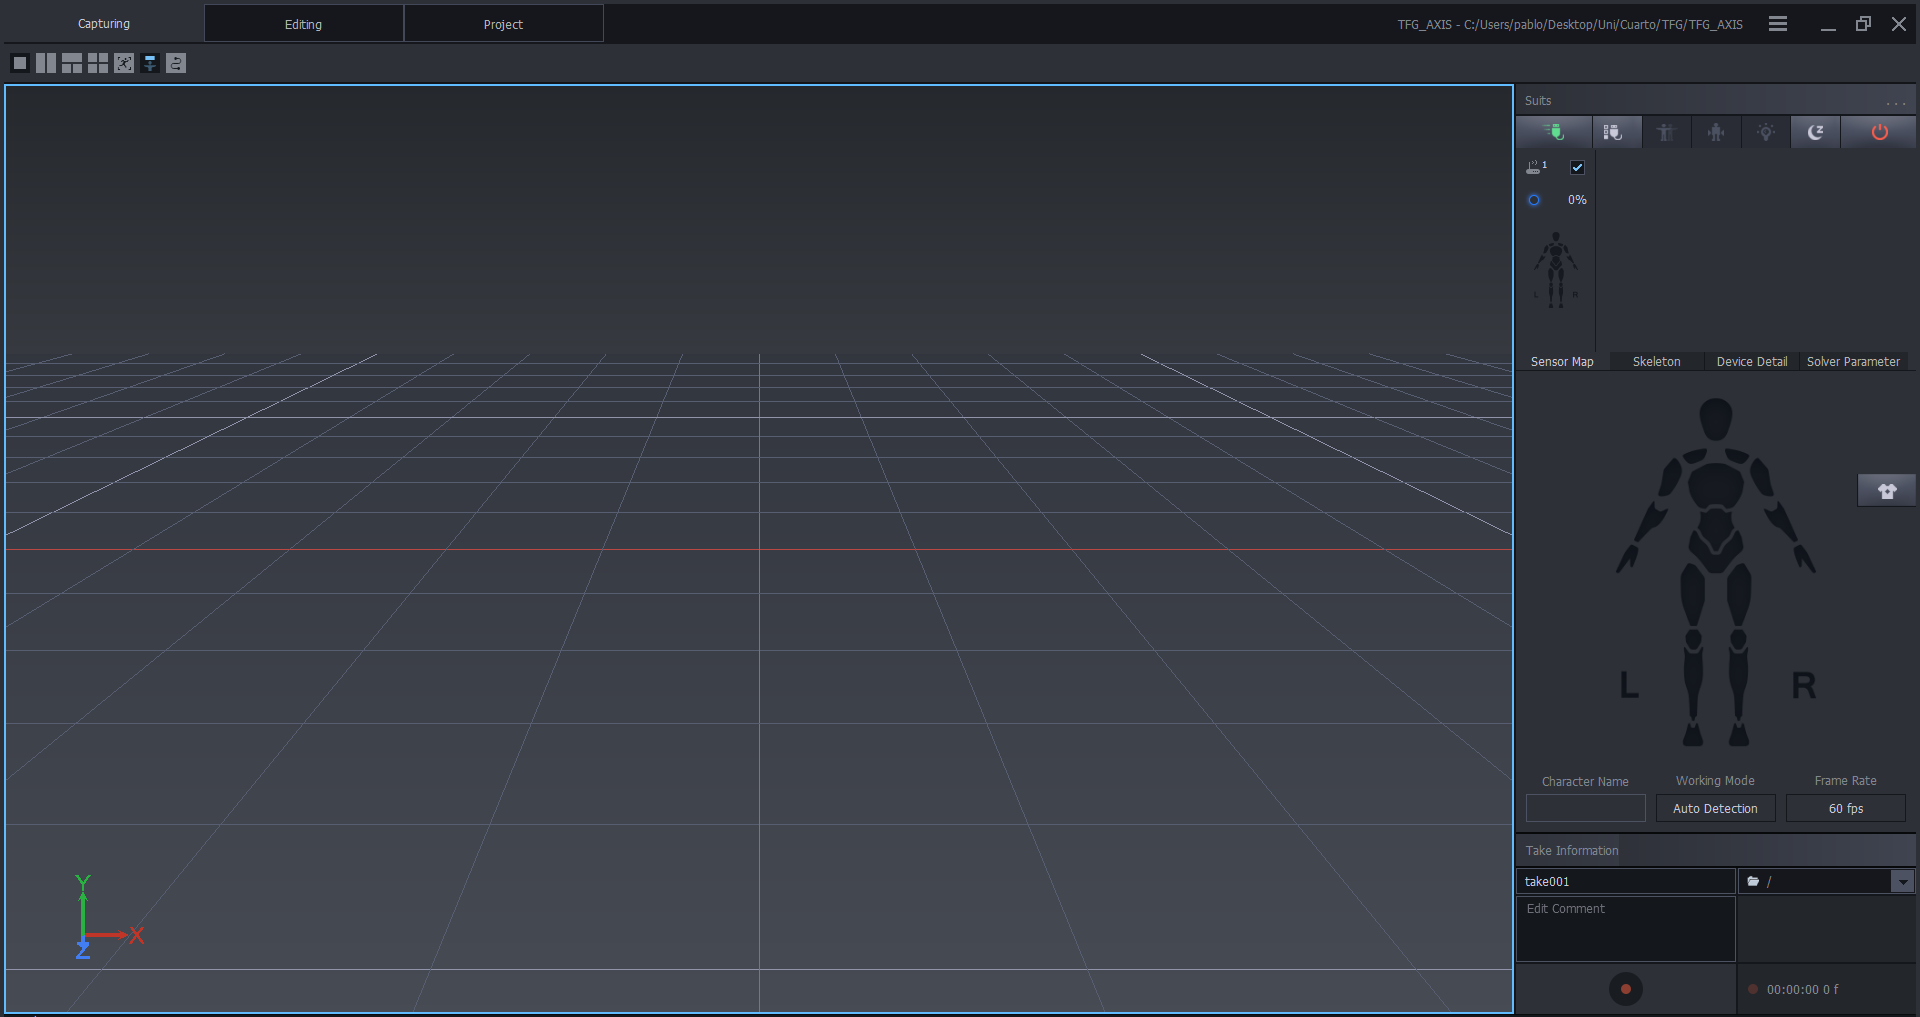
\includegraphics[width=0.5\textwidth]{Imagenes/Bitmap/AxisSinTraje.PNG}
	\caption{Captura de la aplicación Axis Studio antes de conectar un traje}
	\label{fig:AxisSinTraje}
\end{figure}

Para conectar el traje se debe tener enchufado en el mismo equipo el USB receptor y los puertos de carga con los sensores en ellos.
Posteriormente se deben desenchufar los puertos para que el traje se conecte con el receptor, que se muestra con un parpadeo azul en los sensores.

Una vez los sensores puestos en sus huecos de las bandas se debe pulsar al botón mostrado en la figura \ref{fig:BotonConectar} se debe calibrar el traje en el botón mostrado en la figura \ref{fig:BotonCalibrar}.
Esta calibración consiste en tres pasos:
\begin{enumerate}
	\item Posición de T: cabeza recta, piernas rectas paralelas a los hombros y brazos extendidos hacia los lados.
	\item Posición de S: cabeza recta, piernas ligeramente flexionadas, espalda recta y brazos extendidos hacia el frente.
	\item Posición de A: cabeza recta, piernas rectas paralelas a los hombros y brazos relajados paralelos al tronco.
\end{enumerate}

\begin{figure}[H]
	\centering
	
\includegraphics[width=0.5\textwidth]{Imagenes/Bitmap/ConectarTraje.PNG}
	\caption{Captura del botón para conectar el traje a Axis Studio}
	\label{fig:BotonConectar}
\end{figure}

\begin{figure}[H]
	\centering
	
\includegraphics[width=0.5\textwidth]{Imagenes/Bitmap/Calibrar.PNG}
	\caption{Captura del botón para calibrar el traje}
	\label{fig:BotonCalibrar}
\end{figure}

Una vez el traje conectado y calibrado ya puede capturar el movimiento en tiempo real y transmitirlo a Unity.
\subsubsection{Unity y la conexión del traje}
\label{subsec:NeuronMocapLive}
Para poder usar la captura en Unity es necesario el plugin Neuron Mocap Live. \footnote{Enlace a la página de documentación de Neuron Mocap Live: \url{https://support.neuronmocap.com/hc/en-us/sections/206474008-UNITY-SDK}}

Una vez metido el plugin en el proyecto se necesita un objeto vacío que contenga el componente ``Neuron Source Manager''.
Este componente se conecta a la aplicación mediante la dirección IP de la máquina que ejecuta Axis Studio y sockets TCP a un puerto que puedes configurar en la aplicación de Axis Studio mediante el panel que se muestra en la figura \ref{fig:SettingAxis}

\begin{figure}[H]
	\centering
	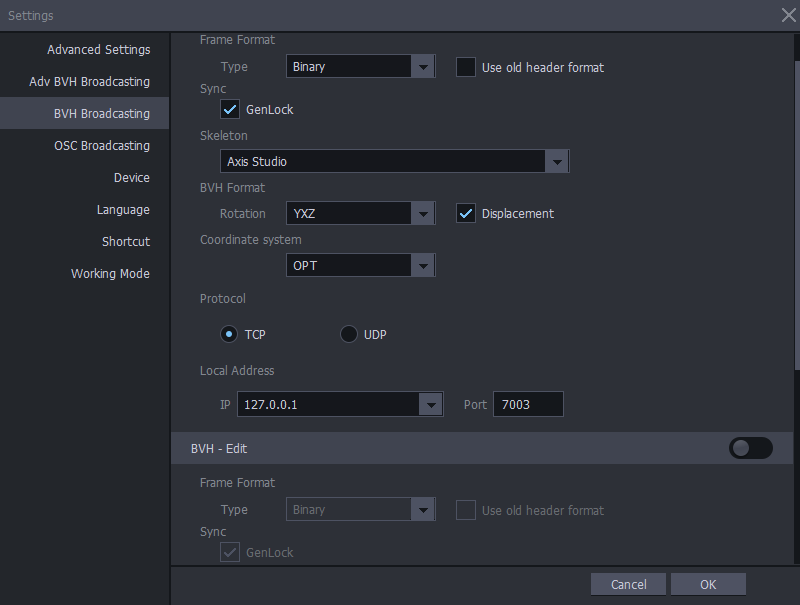
\includegraphics[width=0.5\textwidth]{Imagenes/Bitmap/SettingsAxis.PNG}
	\caption{Captura del panel de configuración de Axis Studio}
	\label{fig:SettingAxis}
\end{figure}

Posteriormente todos los objetos que vayan a usar la captura de movimiento deben ser hijos de este objeto vacío y tener el componente ``Neuron Transforms Instance''.
Este componente tiene una lista de Transforms que usa para mapear los huesos del traje con los del objeto de Unity.

\subsubsection{Limitaciones encontradas con el traje}
Durante el desarrollo del proyecto han habido dos limitaciones con respecto al traje.

La primera de ellos es la ausencia de guantes para capturar los dedos, ya que no vienen incluídos con el traje.
A pesar de que esto causa que los dedos estén siempre en la misma posición con respecto a la mano no ha causado ningún problema en la identificación de gestos

La segunda limiación es la cantidad de ruido electromagnético presente en nuestro espacio de trabajo: la Facultad de Informática de la Universidad Complutense de Madrid.
Este ruido causaba interferencias con el traje, haciendo que la señal con el ordenador fuese pobre constantemente y no se capturasen los movimientos correctamente.

Para solventarlo se requirió de un cable alargador de USB 2.0 de 10 metros que se conectaba al ordenador en el que se enchufaba el receptor y se acercaba lo más posible al traje, ampliando la señal al máximo.

Una vez conectado el traje, solventadas limitaciones y sabiendo los puntos que detecta era necesario un dataset que se puediera acoplar al esqueleto que proporciona el traje.

\subsection{Herramienta de recogida de datos con usuarios reales}
La herramienta se debe conectar con el traje como hemos mencionado anteriormente en el apartado \ref{subsec:NeuronMocapLive}
Una vez conectado se le debe pasar al componente MocapDumper el nombre de la animación que se va a grabar, el número de toma de esa animación y un número que sirva como identifidor de usuario.

Finalmente cuando la herramienta está ejecutándose y se le da a la tecla ``espacio'' genera un CSV del formato ``animación\_User\_Número de ususario\_Take\_Número de toma'' (si el fichero ya existía lo sobreescribe), escribe la misma cabecera del CSV que se menciona en la tabla \ref{tab:cabecera-csv-completa} y pone la aplicación en estado de grabación.
En este estado la aplicación escribe en cada frame todos los componentes de la posición y rotación (en forma de vector de ángulos de Euler) de cada hueso.
Cuando se le vuelve a dar al espacio la aplicación cierra el fichero y vuelve a un estado de no grabación.

En la figura \ref{fig:MocapDumper} se muestra un diagrama de cómo se conectan los diferentes componentes necesarios en esta herramienta

\begin{figure}[H]
	\centering
	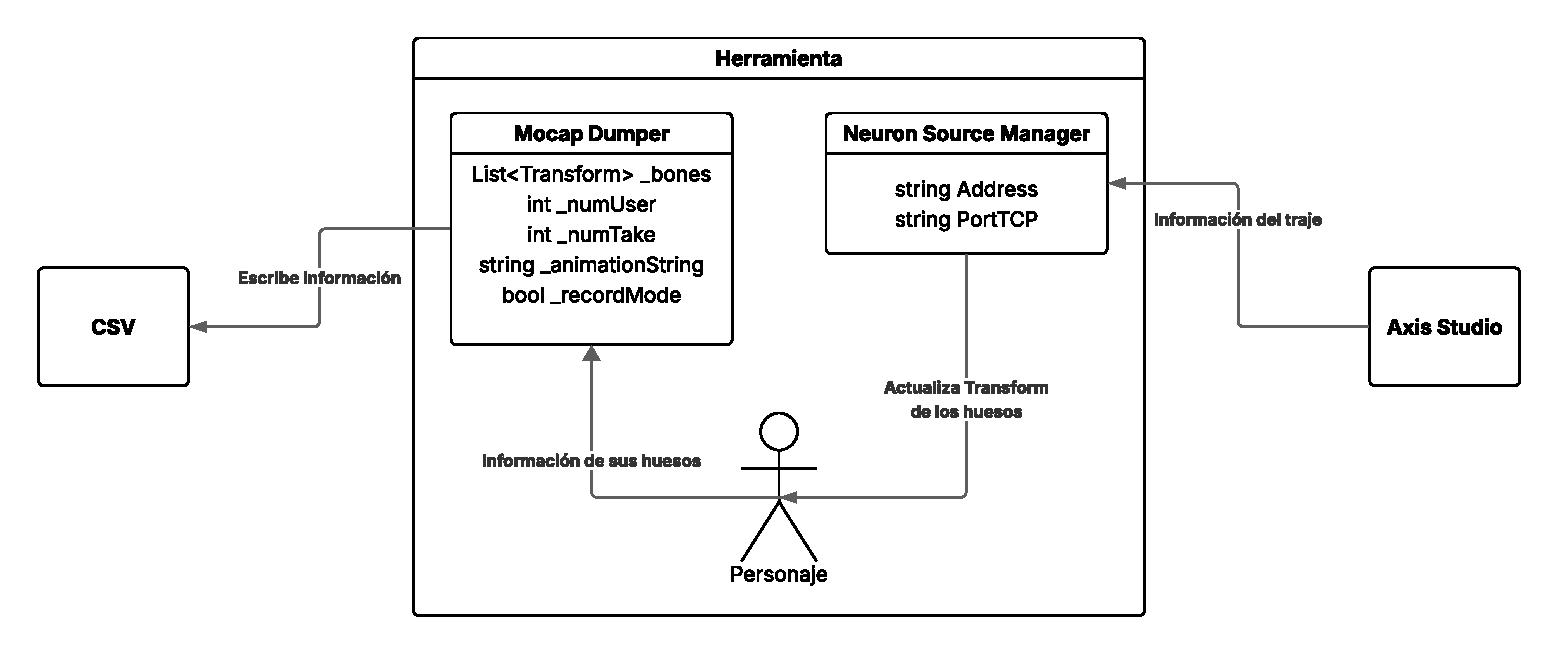
\includegraphics[width=1\textwidth]{Imagenes/Vectorial/MocapDumper.pdf}
	\caption{Diagrama de la conexión entre los distintos componentes de la herramienta, llamada Mocap Dumper}
	\label{fig:MocapDumper}
\end{figure}

\subsection{Recogida de datos}
La recogida de datos consistió en ponerle el traje de captura de movimiento a los usuarios y pedirles que realizasen tres tomas de cada uno de los gestos, a excepción del gesto de baile, ya que de ese gesto había bastantes más datos que el resto.

Para ello se creó un formulario para que los usuarios interesados en ello se apuntasen. En el formulario se explicaba el objetivo de la prueba y se numeraban los datos que iban a ser pedidos en la prueba. Los campos a rellenar eran: correo, consentimiento informado de la recogida de datos posterior y posibles huecos libres (en un horario de lunes a viernes, de 9:00 a 20:00 en espacios de una hora).

El formulario se puede ver en las capturas de pantalla del apéndice \ref{appendix:formularioCitas}. Este formulario y el de demografía fueron comprobados por María del Carmen Fernández Villalba, Responsable de Protección de datos en Vicepresidencia Primera, perteneciente a Presidencia de La Junta de Comunidades de Castilla La Mancha, dado que no se quería vulnerar la Ley de Protección de Datos de ninguna manera.

Una vez creado el formulario se creó una selección de carteles (figuras \ref{fig:cartel-facultad}, \ref{fig:cartel-redes}, \ref{fig:cartel-pantallas}) el cual se colgó en redes y se colgó en distintas facultades, teniendo como resultado que se apuntasen 75 personas en el formulario.

Lo siguiente era tener un sitio en el que hacer las pruebas. Debido a que las pruebas requerían movimiento era preciso un lugar en el que los usuarios se pudiesen mover sin dificultades y que no estuviese a la vista para preservar la intimidad de los mismos.

Una vez se cerró el formulario, se procedió a hacer un algoritmo que asignara la mayor cantidad de citas posibles dadas las restricciones de tiempo de los usuarios y los días disponibles. El algoritmo\footnote{Enlace al algoritmo: \url{https://github.com/FratosVR/Models/blob/main/citas_generacion_dataset/Scheduler.py}} usa un esquema de ramificación y poda para conseguir la combinación con mayor cantidad de citas disponibles sin tardar más de 10 segundos en procesar las combinaciones válidas.

Finalmente desde el día 14/04/2025 a las 9:00 hasta el día 17/04/2025 a las 19:30 se pudo grabar en el despacho 216 (Sala de grabaciones) de la Facultad de Informática de la Universidad Complutense de Madrid.
De los 75 usuarios apuntados finalmente se presentaron 65, consiguiendo así 975 animaciones en formato CSV, 195 de cada gesto. En la figura \ref{fig:PruebasLidia} se muestra una fotografía de un usuario durante el proceso de calibración.

\begin{figure}[H]
	\centering
	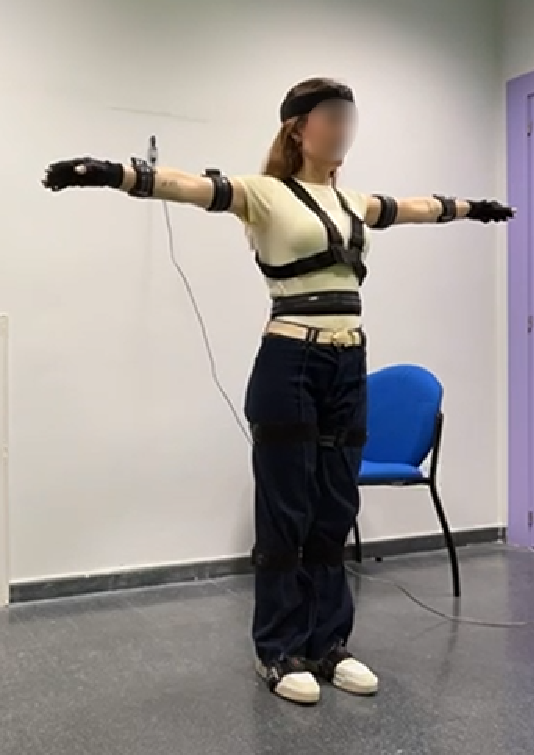
\includegraphics[width=0.5\textwidth]{Imagenes/Vectorial/LidiaPruebasBlurr.pdf}
	\caption{Fotografía de un usuario en las pruebas}
	\label{fig:PruebasLidia}
\end{figure}

A los usuarios no solo se les pidió que realizaran gestos, sino que también se les pidió una serie de información demográfica de manera anónima para saber como de representativa era la muestra. La información pedida fue: género, edad, nacionalidad (o nacionalidades), idiomas hablados y mano dominante.

Este formulario se puede ver en el apéndice \ref{appendix:formularioDemografia}

Estos datos se recogieron con la cuenta de Google de las personas que llevaban el formulario, por lo que no se guardó ningún dato identificable de ningún usuario. En la categoría de género(figura \ref{fig:muestreo-genero}) podemos ver que los datos son un 43.1\% femenino, 50.8\% masculino y 6.2\% no binario. La edad(figura \ref{fig:muestreo-edad}) más común es de 21, con un recuento de un 26.2\% de los encuestados. La nacionalidad (figura \ref{fig:muestreo-nacionalidad}) más común es la española, con un 89.23\% de los encuestados. En la figura \ref{fig:muestreo-idiomas} se puede ver que el idioma más hablado es el español, con un 100\% de los encuestados, seguido de inglés y francés. En la figura \ref{fig:muestreo-mano} se puede ver que el 93.85\% de los encuestados son diestros.

Tras las recogida de datos, se siguió el mismo proceso de estandarización de datos que se usó en el dataset artificial. Antes de estandarizar los datos parecía que se había conseguido eliminar el gran desbalance del dataset hacia los gestos de baile, tras la estandarización de los datos, se vió que las animaciones de baile seguían ganando en cantidad por mucho respecto a las otras. La comparativa se puede ver en las figuras \ref{fig:datos-bruto} y \ref{fig:datos-estandar}.

\begin{figure}[H]
	\centering
	\includegraphics[width=0.7\textwidth]{Imagenes/Bitmap/Distribución_de_animaciones_en_bruto_por_categoria.png}
	\caption{Distribución de los datos brutos}
	\label{fig:datos-bruto}
\end{figure}

\begin{figure}[H]
	\centering
	\includegraphics[width=0.7\textwidth]{Imagenes/Bitmap/Distribución_de_animaciones_adaptadas_por_categoria.png}
	\caption{Distribución de los datos estandarizados}
	\label{fig:datos-estandar}
\end{figure}

El resultado final de todos los datos se puede ver en \cite{csv-pose-animations}. Una vez recogidos y procesados los datos recogidos en las pruebas de usuario se procede al entrenamiento de los distintos modelos para su posterior comparativa.
\section{Modelos de \gls{ia}}

Tras la adaptación y guardado de datos, se procede al desarrollo de los modelos de \gls{ia}. Este desarrollo no implica solo el modelo, sino también la creación de una interfaz de entrenamiento y visualizado de resultados(para los modelos que lo permiten). Durante todo el proceso se han usado las siguientes tecnologías:
\begin{itemize}
    \item \textbf{Python}
    \item \textbf{Tensorflow}
    \item \textbf{TensorBoard}
    \item \textbf{Tensorflow Serving}
    \item \textbf{Keras}
    \item \textbf{Pandas}
    \item \textbf{Numpy}
    \item \textbf{Matplotlib}
    \item \textbf{Scikit-learn}
    \item \textbf{YDF}
    \item \textbf{Gradio}
    \item \textbf{Kaggle}
    \item \textbf{Jupyter Notebook}
\end{itemize}

En el repositorio\footnote{Enlace al repositorio de GitHub \url{https://github.com/FratosVR/Models}} se puede encontrar el código de todos los modelos y su entrenamiento, así como algunos modelos ya preentrenados. Durante esta sección se explicará el proceso de desarrollo de cada parte del proyecto.

\subsection{Interfaz de entrenamiento y seguimiento}

Al principio del desarrollo, surgió la necesidad de hacer que el entrenamiento de los modelos fuera accesible para gente que nunca hubiera trabajado con \gls{ia} o Python. Esto ocurre debido a que se ideó una comparativa de modelos, y los ordenadores disponibles no daban la talla para entrenar los modelos en el tiempo necesario. Por esto se pidió como favor a la asociación LAG (asociación de estudiantes de la Facultad de informática de la UCM) el poder usar sus equipos con mejores gráficas para llevar a cabo estos entrenamientos.

Se usó Gradio(\cite{Abid_Gradio_Hassle-free_sharing_2019}) para crear una interfaz web accesible para cualquier persona. En un primer momento esta interfaz solo contaba con una pantalla en la que había:
\begin{itemize}
    \item Un selector de tipo de modelo
    \item Un área de texto para introducir la ruta al conjunto de datos
    \item Un \textit{slider} para seleccionar el intervalo de tiempo entre los frames de animación
    \item Un botón para seleccionar todos los posibles intervalos de tiempo
    \item Un botón para iniciar el entrenamiento
    \item Un área de archivo para descargar el modelo entrenado
    \item Un área de imagen para mostrar la matriz de confusión tras el entrenamiento
    \item Un área de texto para mostrar el resultado del entrenamiento
\end{itemize}

Esta interfaz (figura \ref{fig:interfaz-train}) se hizo lo mas simple posible para que un usuario estándar pudiera poner a entrenar un modelo sin tener que tocar nada de código. Sólo se tienen que seleccionar el modelo y el intervalo deseado, introducir la ruta al \textit{dataset} y esperar a que termine.
\begin{figure}[h!]
    \centering
    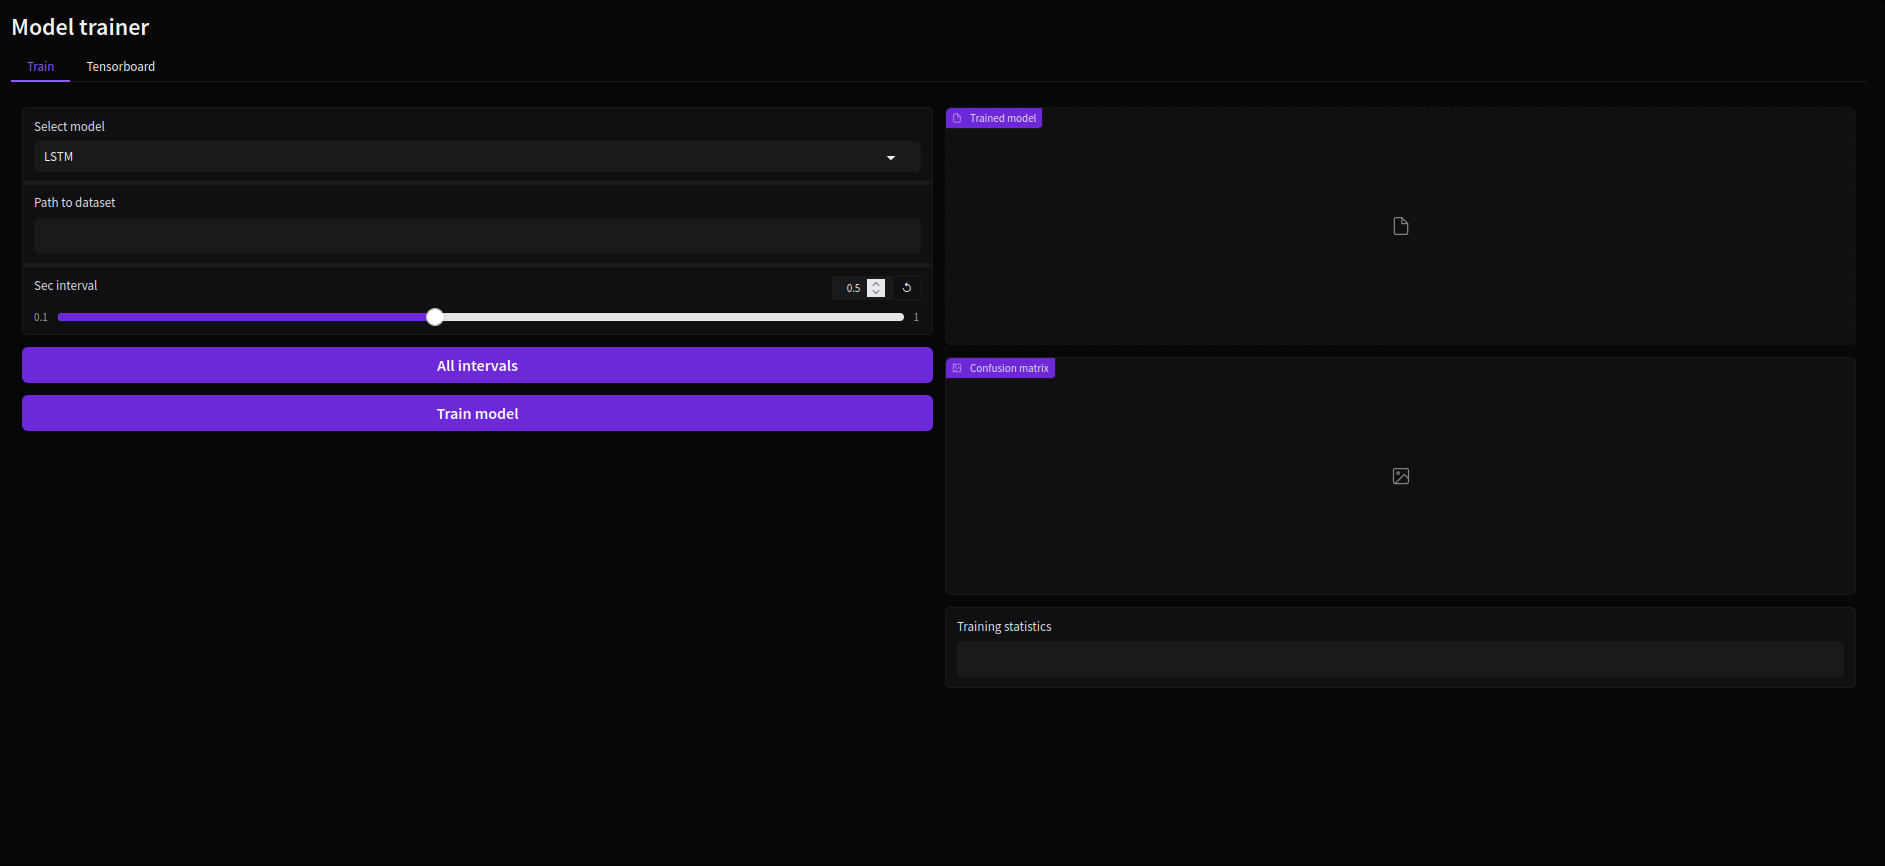
\includegraphics[width=0.9\textwidth]{Imagenes/Bitmap/interfaz-train.png}
    \caption{Interfaz de entrenamiento}
    \label{fig:interfaz-train}
\end{figure}


La función de entrenamiento que se ejecuta al pulsar el botón ``Train model'' hace lo siguiente:
\begin{enumerate}
    \item Se crea un entrenador del modelo seleccionado
    \item Se crea un objeto \textit{DataLoader} que se encargará de cargar los datos con el intervalo de tiempo de separación seleccionado.
    \item Se separan los datos cargados en 60\% para entrenamiento, 20\% para validación y 20\% para test. Se consideró hacer cross validation, pero los tiempos de entrenamiento ya eran demasiado largos para los modelos neuronales.
    \item Se pasan las categorías con \textit{OneHotEncoder} para que el modelo pueda entenderlas.
    \item Se entrena el modelo con los datos de entrenamiento y validación.
    \item Se guarda el modelo.
    \item Se comprueba cual es el mejor modelo entrenado entre todos los intervalos de tiempo seleccionados.
    \item Se muestra la matriz de confusión en la interfaz, el archivo del modelo y sus estadisticas.
\end{enumerate}

En la parte superior izquierda se puede ver dos secciones: ``Train'' y ``TensorBoard''. La sección ``Train'' es la explicada anteriormente, la sección ``TensorBoard'' es una sección que permite ver el progreso del entrenamiento en tiempo real. No solo eso, sino que también nos permite ver el rendimiento de modelos ya entrenados y ver como los hiperparámetros han afectado a su tasa de acierto. TensorBoard permite añadir funciones al código de entrenamiento para modificar el comportamiento del método de entrenamiento y dejar constancia de las distintas partes del mismo. Esta interfaz se puede ver en la figura \ref{fig:interfaz-tensorboard}.

\begin{figure}[h!]
    \centering
    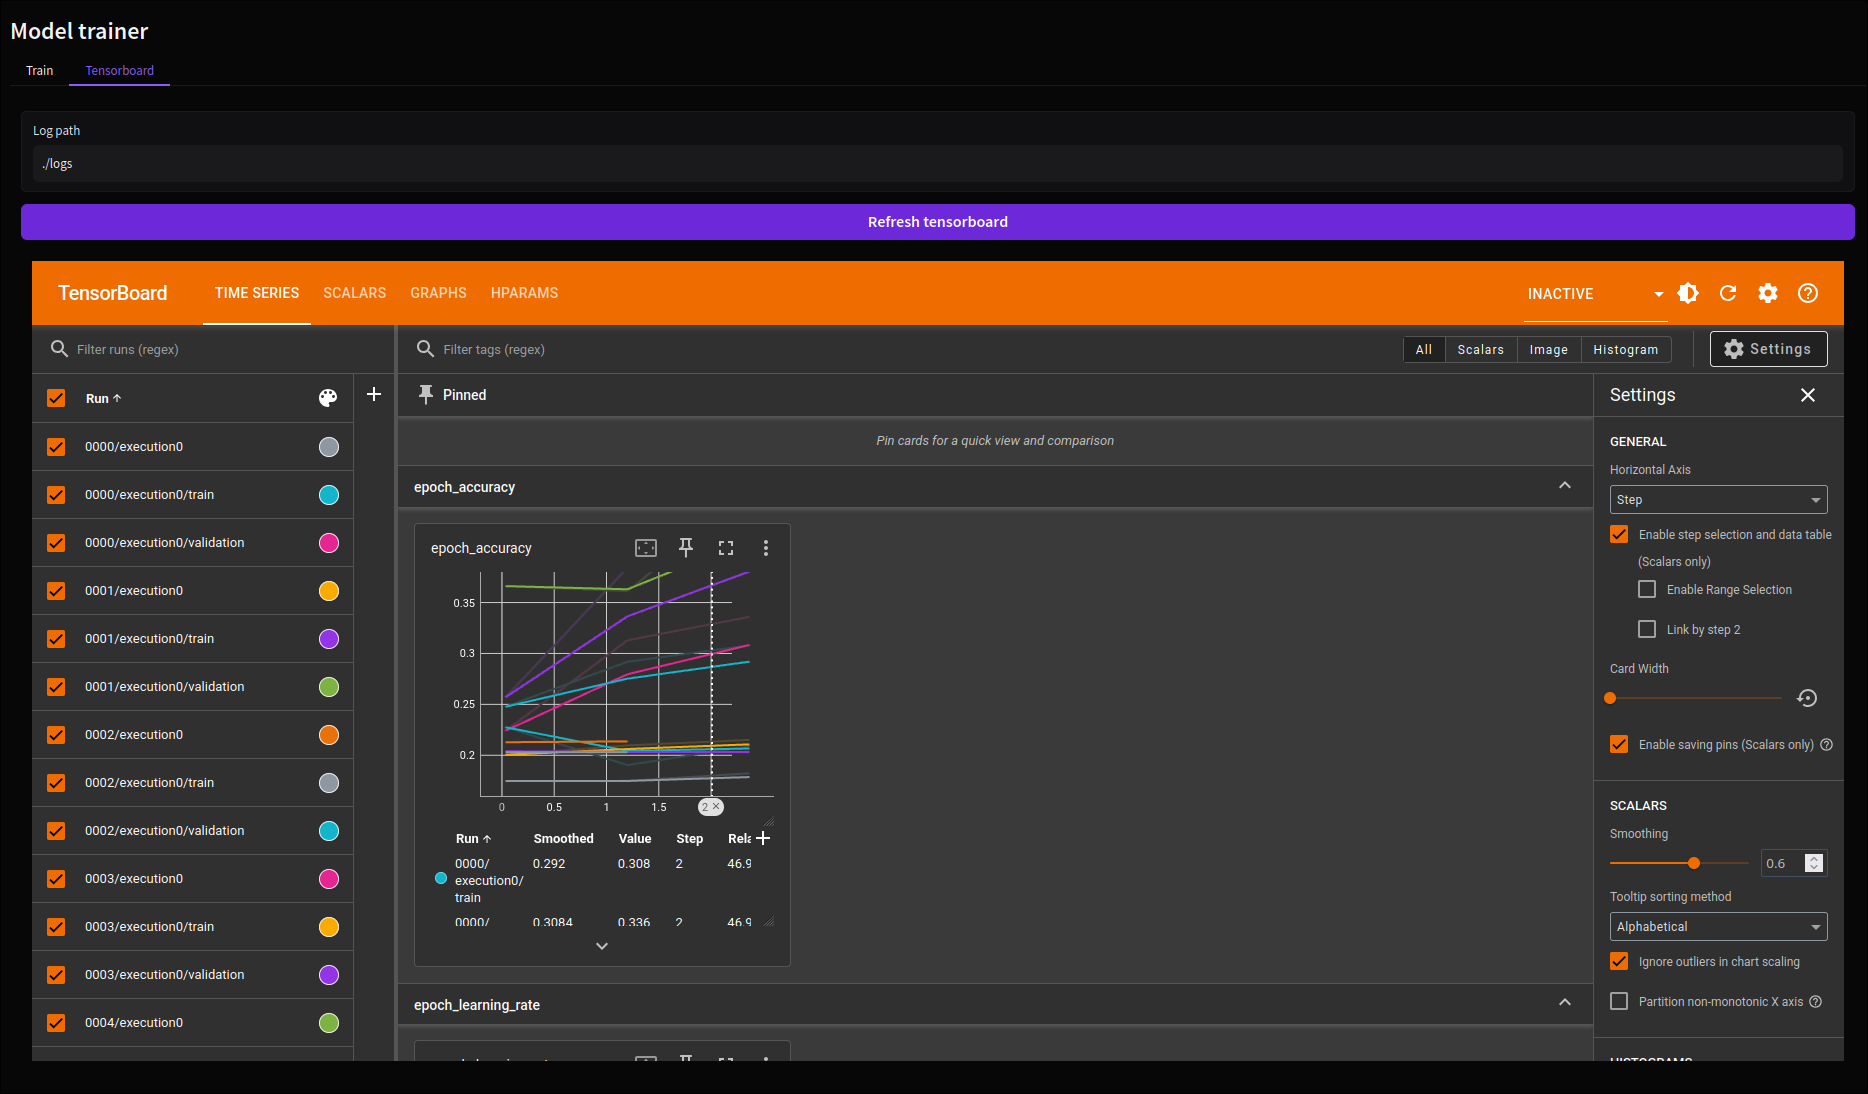
\includegraphics[width=0.9\textwidth]{Imagenes/Bitmap/interfaz-tensorboard.png}
    \caption{Interfaz de TensorBoard}
    \label{fig:interfaz-tensorboard}
\end{figure}

Para todo lo descrito, el archivo ``Interface.py'' tiene la estructura presentada en la figura \ref{fig:interfaz-estructura}. Las funciones \_\_change\_interval y \_\_change\_interval\_all cambian los intervalos de tiempo usados dentro del entrenamiento, \_\_setup\_ui crea el \textit{layout} de la interfaz, \_\_refresh\_tensorboard cambia la ruta de los \textit{logs} de TensorBoard y recarga el \gls{iframe}. El método \_\_train ejecuta todo el proceso de entrenamiento previamente descrito.

\begin{figure}[h!]
    \centering
    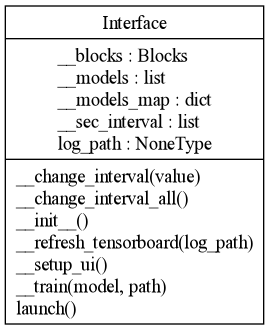
\includegraphics[width=0.3\textwidth]{Imagenes/Bitmap/classes_Interface.png}
    \caption{Estructura del archivo de la interfaz}
    \label{fig:interfaz-estructura}
\end{figure}

\subsection{Carga de datos}

La carga de datos se gestiona con la clase \textit{DataLoader}. Esta clase se mencionó en el apartado del dataset artificial ya que es la misma que se encarga de estandarizar los datos. Cuando se llama a la función de inicio de la clase se le pasa un intervalo de tiempo, este intervalo marca la distancia entre frames que se va a cargar. Si le indicamos una distancia de 0.8, cargará el frame 0 y el 72. Esto nos permite entrenar distintos modelos con distintas ventanas de envío de datos para comprobar si hay alguna diferencia en el rendimiento.

Estos datos una vez cargados se envían como una lista de tuplas <tipo\_animacion, lista\_de\_frames>. Tras esto, el objeto que reciba estos datos ya puede transformarlos como sea necesario y separarlos en entrenamiento, test y validación.

\subsection{Modelos usados}

A la hora de escoger modelos para la comparativa, se tuvo en cuenta el estudio \cite{combining3dskeleton} como un referente. Se tuvo siempre en cuenta que se intentaba buscar un modelo con el cómputo más simple posible para que fuera lo más accesible para cualquier tipo de máquina. Valorando también las dificultades de tiempo que conlleva el entrenamiento de modelos al final se consideró probar tres redes neuronales usadas para series temporales y un modelo clásico de clasificación.

En un primer momento se pensó también en modelos como \gls{yolo}, pero al ser un modelo basado en imágenes y el estudio plantearse con un traje de captura de movimiento, se decidió que sería una carga muy grande para las aplicaciones que usaran el modelo resultante por tener que renderizar una segunda cámara constantemente para el usuario. Otros modelos como \gls{svm} o \gls{knn} fueron descartados por falta de tiempo de entrenamiento.
\subsubsection{\gls{lstm}}

Este primer modelo va a servir para ilustrar como funcionan el resto de modelos basados en redes neuronales en este estudio. La estructura de la clase \textit{LSTMTrainer} se puede ver en la figura \ref{fig:lstm-estructura}. La mayoría de los atributos privados de la clase son los hiperparámetros del modelo, los otros atributos se usan para guardar información o para guardar el mecanismo usado para buscar hiperparámetros óptimos.

La función train\_with\_hparams se encarga de generar modelos con distintos hiperparámetros y entrenarlos para buscar el mejor. Para que este mecanismo fuera lo más eficiente posible, se ha hecho uso de la biblioteca keras-tuner (\cite{omalley2019kerastuner}), un \textit{framework} de búsqueda de hiperparámetros con distintos algoritmos de búsqueda ya implementados. Tras leer el arctículo \cite{li2018hyperbandnovelbanditbasedapproach} se optó por usar el algoritmo Hyperband, dado que los inconvenientes que presenta no representan un problema comparado con las ventajas de velocidad y eficiencia que otorga.

Esta búsqueda de hiperparámetros se centra en los siguientes:
\begin{itemize}
    \item \textbf{activation}: Función de activación de la capa oculta.
    \item \textbf{dropout}: Porcentaje de \textit{dropout} de la capa oculta.
    \item \textbf{recurrent\_activation}: Función de activación de la capa recurrente.
    \item \textbf{recurrent\_dropout}: Porcentaje de \textit{dropout} de la capa recurrente.
    \item \textbf{unroll}: Si se usa el \textit{unroll} de la capa LSTM.
    \item \textbf{use\_bias}: Si se usa el \textit{bias} de la capa LSTM.
\end{itemize}

El entrenamiento crea un modelo con los hiperparámetros seleccionados dentro de un rango, se entrena durante unas épocas y se comprueban resultados. Se pasa a otro conjunto de hiperparámetros y así hasta completarlos todos. Tras esto, se aumenta el número de épocas y se siguen entrenando los anteriores modelos. Tras acabar de entrenar todos los modelos, se selecciona el que mejor precisión en validación tenga.

De este ``mejor modelo'' se crea una matriz de confusión, se guarda el modelo en formato keras y se envían las estadísticas a la interfaz de gradio. Todo este proceso queda registrado en TensorBoard gracias a la lilbrería \textit{HParams} (\cite{hparams}).

\begin{figure}[h!]
    \centering
    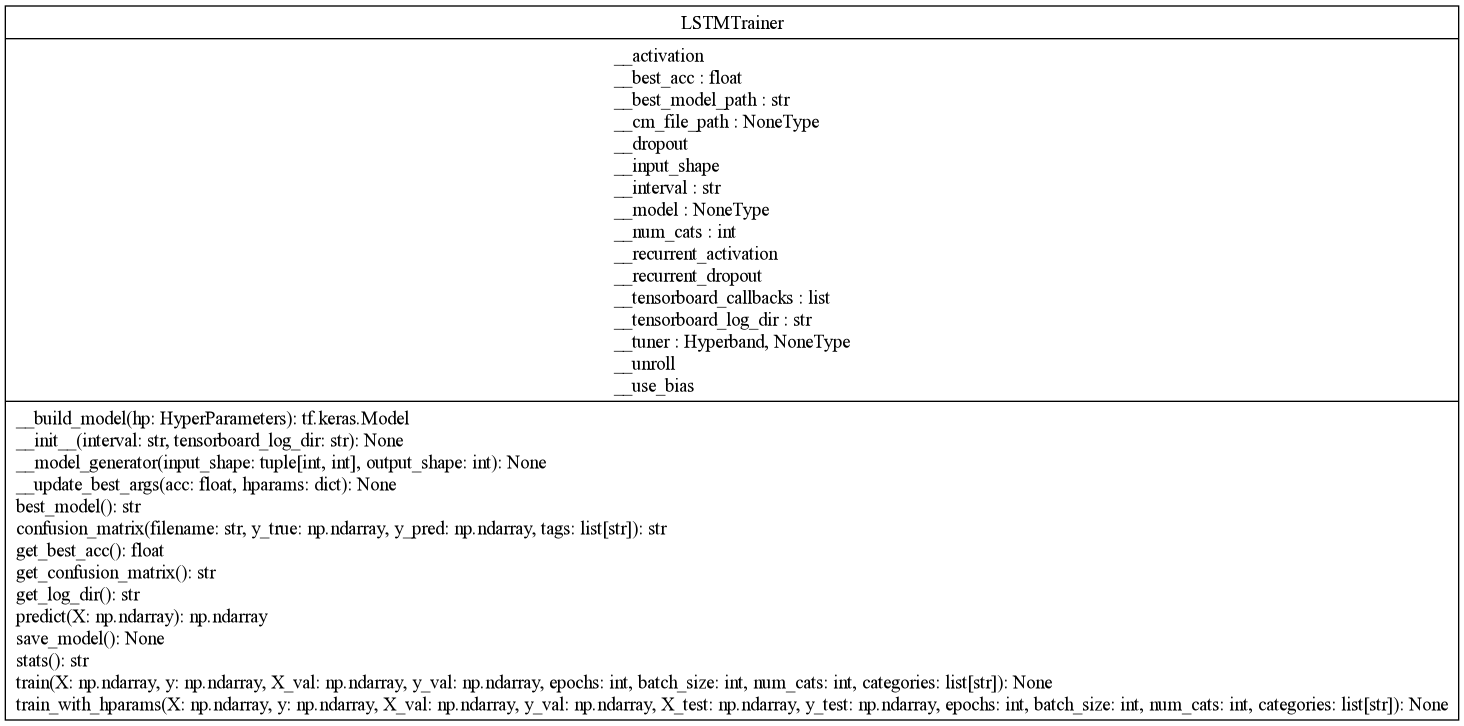
\includegraphics[width=0.8\textwidth]{Imagenes/Bitmap/classes_LSTMTrainer.png}
    \caption{Estructura de la clase LSTMTrainer}
    \label{fig:lstm-estructura}
\end{figure}

El modelo \gls{lstm} usado es un \textit{Sequential} de keras con una capa LSTM y una capa densa. La capa LSTM con los hiperparámetros antes descritos y la capa densa tiene tamaño el número de categorías de animaciones y una activación softmax. El modelo se compila utiliando el optimizador \textit{Adam}, la perdida se calcula con \textit{categorical\_crossentropy} y la métrica de evaluación es la \textit{accuracy}. Durante el proceso de entrenamiento se usan los \textit{callbacks} de \textit{EarlyStopping} para ahorrar recursos en entrenamientos que no parecen mejorar y los \textit{callbacks} de \textit{TensorBoard} para guardar los logs de entrenamiento y poder verlos en la interfaz de TensorBoard.

Entre los modelos de \gls{lstm} entrenados, el del intervalo de 0.8 fue el que mejor rendimiento tuvo, con una precisión de 0.51025 en entrenamiento y 0.5912 en validación. A continuación se puede ver el esquema del modelo en la figura \ref{fig:lstm-0.8-ejemplo}, la matriz de confusión en la figura \ref{fig:lstm-0.8-matriz-ejemplo} y el gráfico de entrenamiento en la figura \ref{fig:lstm-0.8-grafico-ejemplo}. Podemos ver en la matriz de confusión que los gestos menos reconocidos son baile y saludo. Los resultados del resto de intervalos se pueden ver en el apéndice \ref{appendix:resultadosLSTM}.

\begin{figure}[h!]
    \centering
    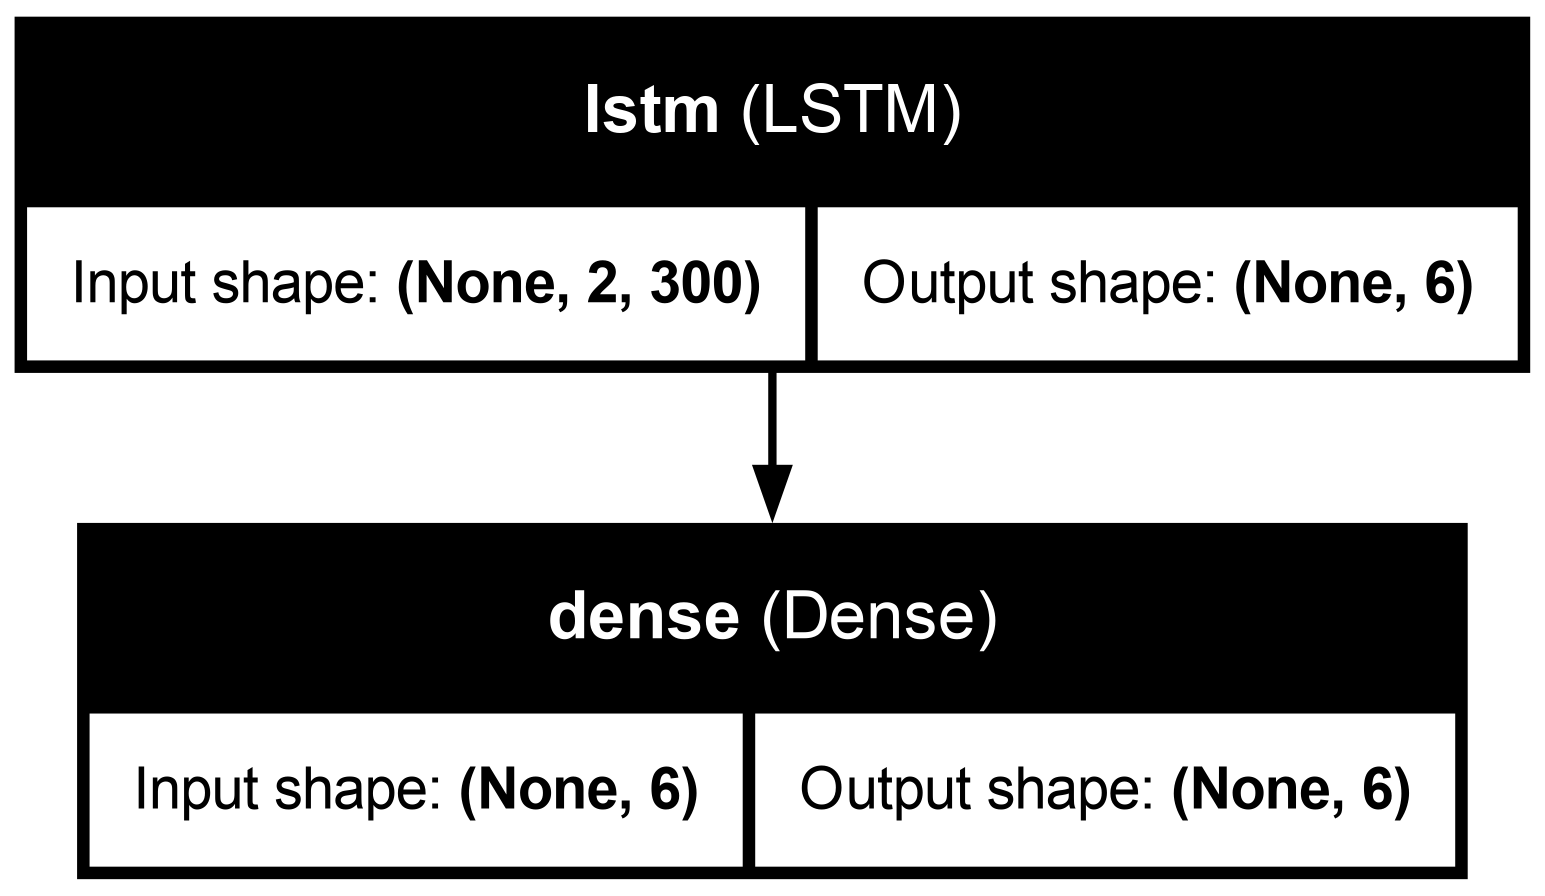
\includegraphics[width=0.8\textwidth]{Imagenes/Bitmap/best-lstm0.8.png}
    \caption{Esquema del modelo LSTM}
    \label{fig:lstm-0.8-ejemplo}
\end{figure}
\begin{figure}[h!]
    \centering
    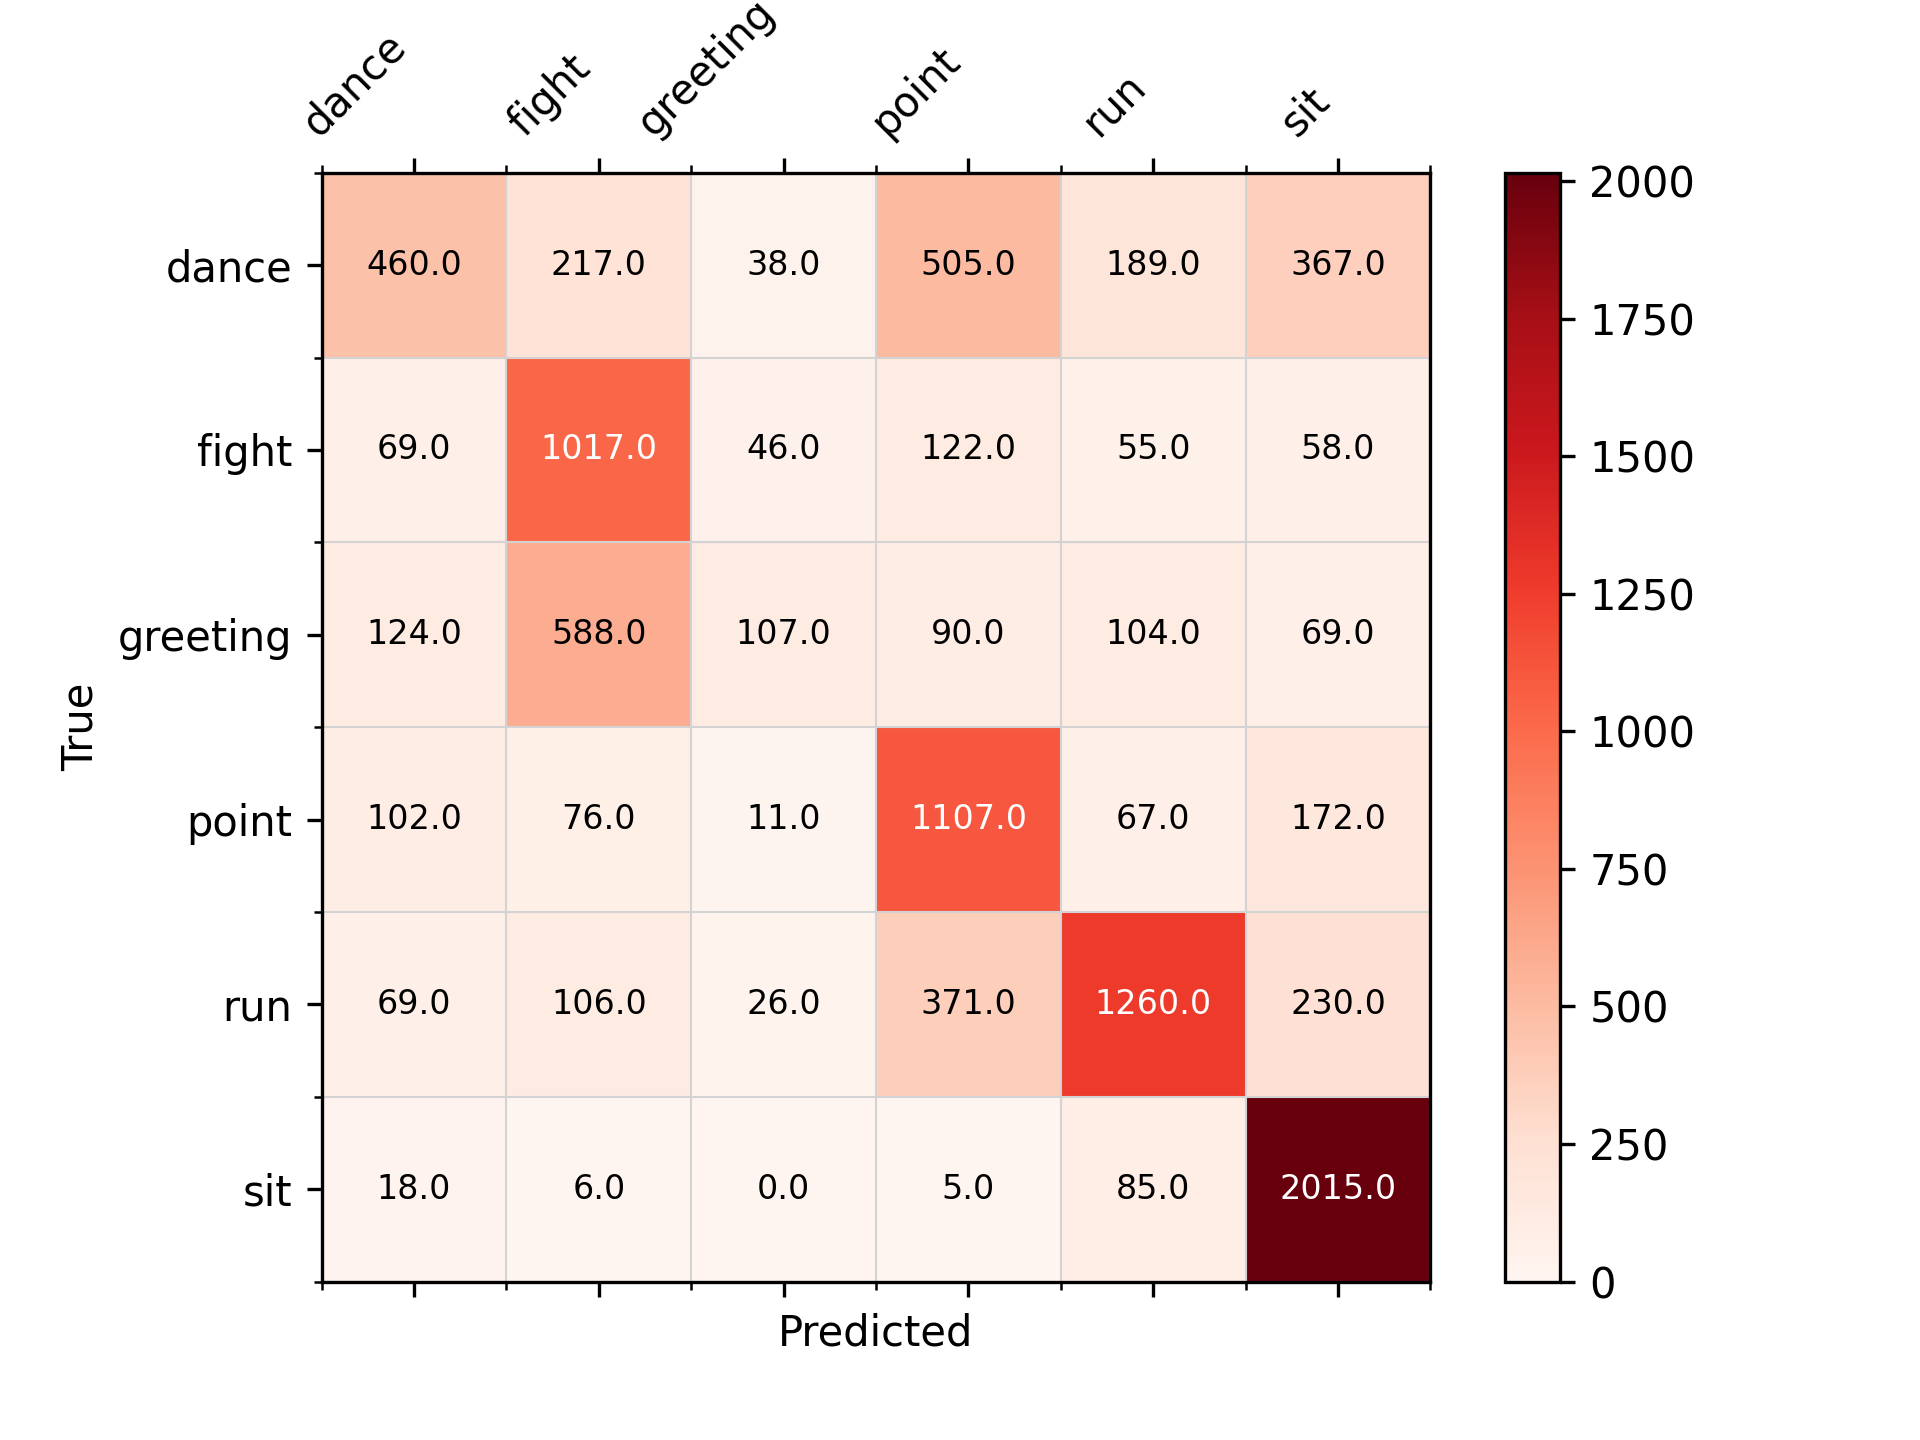
\includegraphics[width=0.8\textwidth]{Imagenes/Bitmap/CM_best-lstm0.8.png}
    \caption{Matriz de confusión del modelo LSTM}
    \label{fig:lstm-0.8-matriz-ejemplo}
\end{figure}
\begin{figure}[h!]
    \centering
    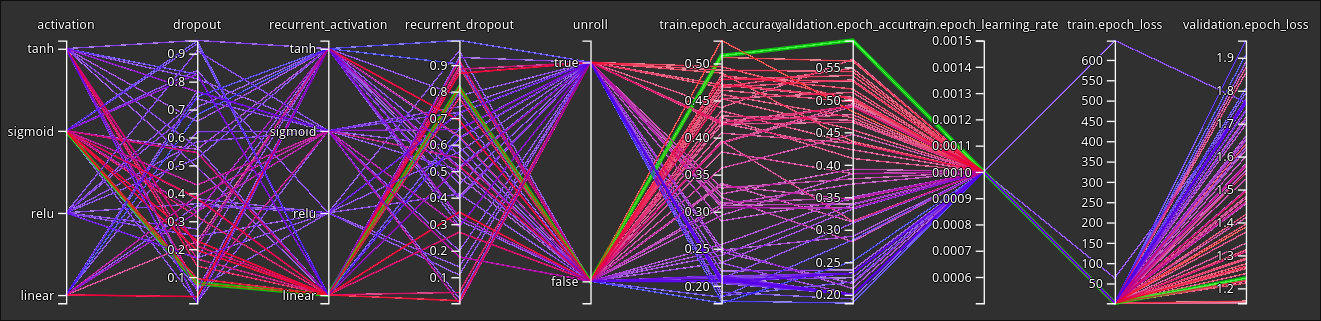
\includegraphics[width=0.8\textwidth]{Imagenes/Bitmap/tb-lstm-0.8.png}
    \caption{Gráfico de entrenamiento del modelo LSTM}
    \label{fig:lstm-0.8-grafico-ejemplo}
\end{figure}

\subsubsection{\gls{cnn}}


El modelo de \gls{cnn} se entrenó de una manera muy similar al de \gls{lstm}. En el uml de la figura \ref{fig:cnn-estructura} se puede ver la estructura de la clase \textit{CNNTrainer}, la cual es muy similar a la de \textit{LSTMTrainer}. La diferencia está en los hiperparámetros buscados. Estos son:
\begin{itemize}
    \item \textbf{activation}: Función de activación de la capa oculta.
    \item \textbf{conv\_filters}: Número de filtros de la capa convolucional.
    \item \textbf{dense\_units}: Número de neuronas de la capa densa.
    \item \textbf{dropout}: Porcentaje de \textit{dropout} de la capa oculta.
    \item \textbf{kernel\_size}: Tamaño del kernel de la capa convolucional.
    \item \textbf{pool\_size}: Tamaño del \textit{pooling} de la capa convolucional.
\end{itemize}

\begin{figure}[h!]
    \centering
    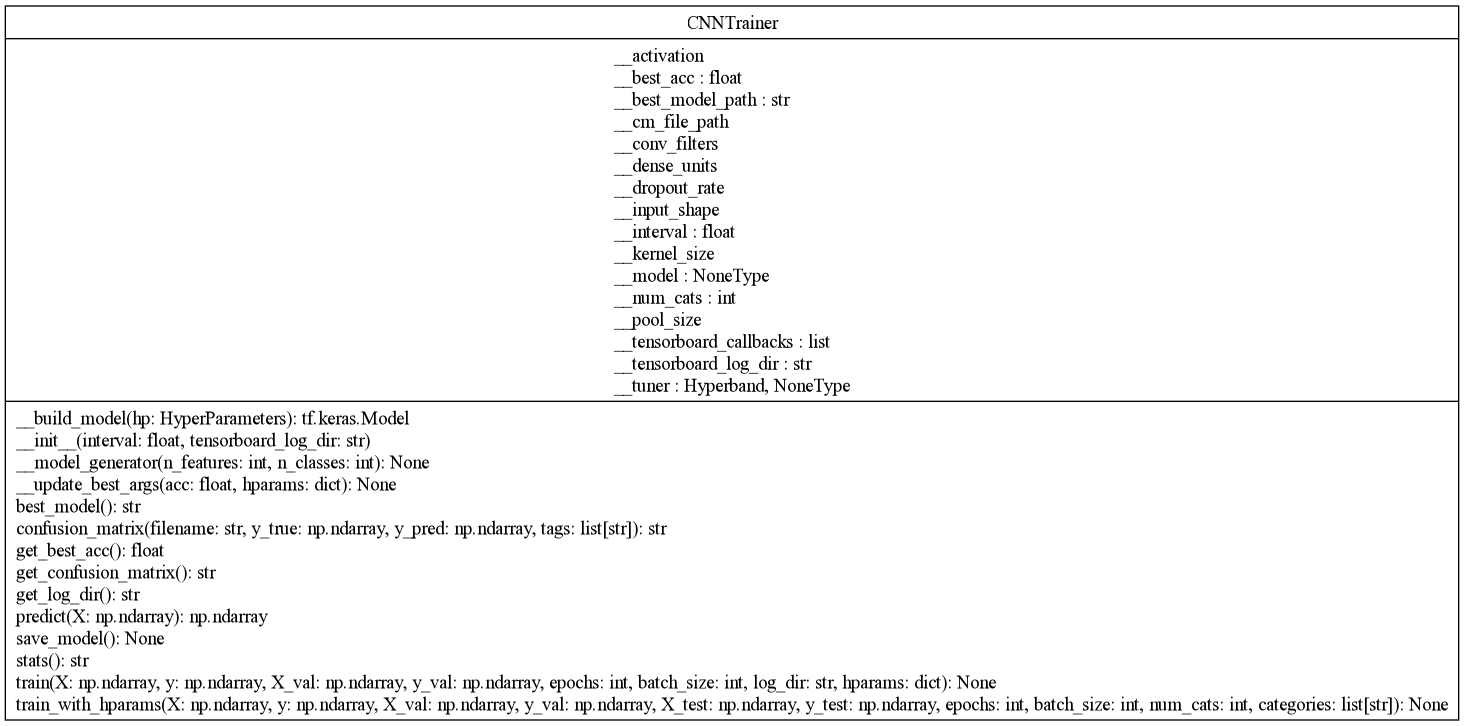
\includegraphics[width=0.8\textwidth]{Imagenes/Bitmap/classes_CNNTrainer.png}
    \caption{Estructura de la clase CNNTrainer}
    \label{fig:cnn-estructura}
\end{figure}

El método de entrenamiento es el mismo que el descrito en el apartado anterior, haciendo uso de keras-tuner para encontrar los mejores hiperparámetros. En el caso de este modelo, el mejor resultado se consigue con el intervalo de 1 segundo, haciendo este modelo más un reconocedor de poses que de gestos, con una precisión de 0.55879 en entrenamiento y 0.56002 en validación. En la figura \ref{fig:cnn-1.0-ejemplo} se puede ver el esquema del modelo, en la figura \ref{fig:cnn-1.0-matriz-ejemplo} la matriz de confusión y en la figura \ref{fig:cnn-1.0-grafico-ejemplo} el gráfico de entrenamiento. En este caso podemos ver que los gestos que peor detecta son baile y saludo (siendo saludo muy confundido con pelea). Los resultados del resto de intervalos se pueden ver en el apéndice \ref{appendix:resultadosCNN}.
\begin{figure}[H]
    \centering
    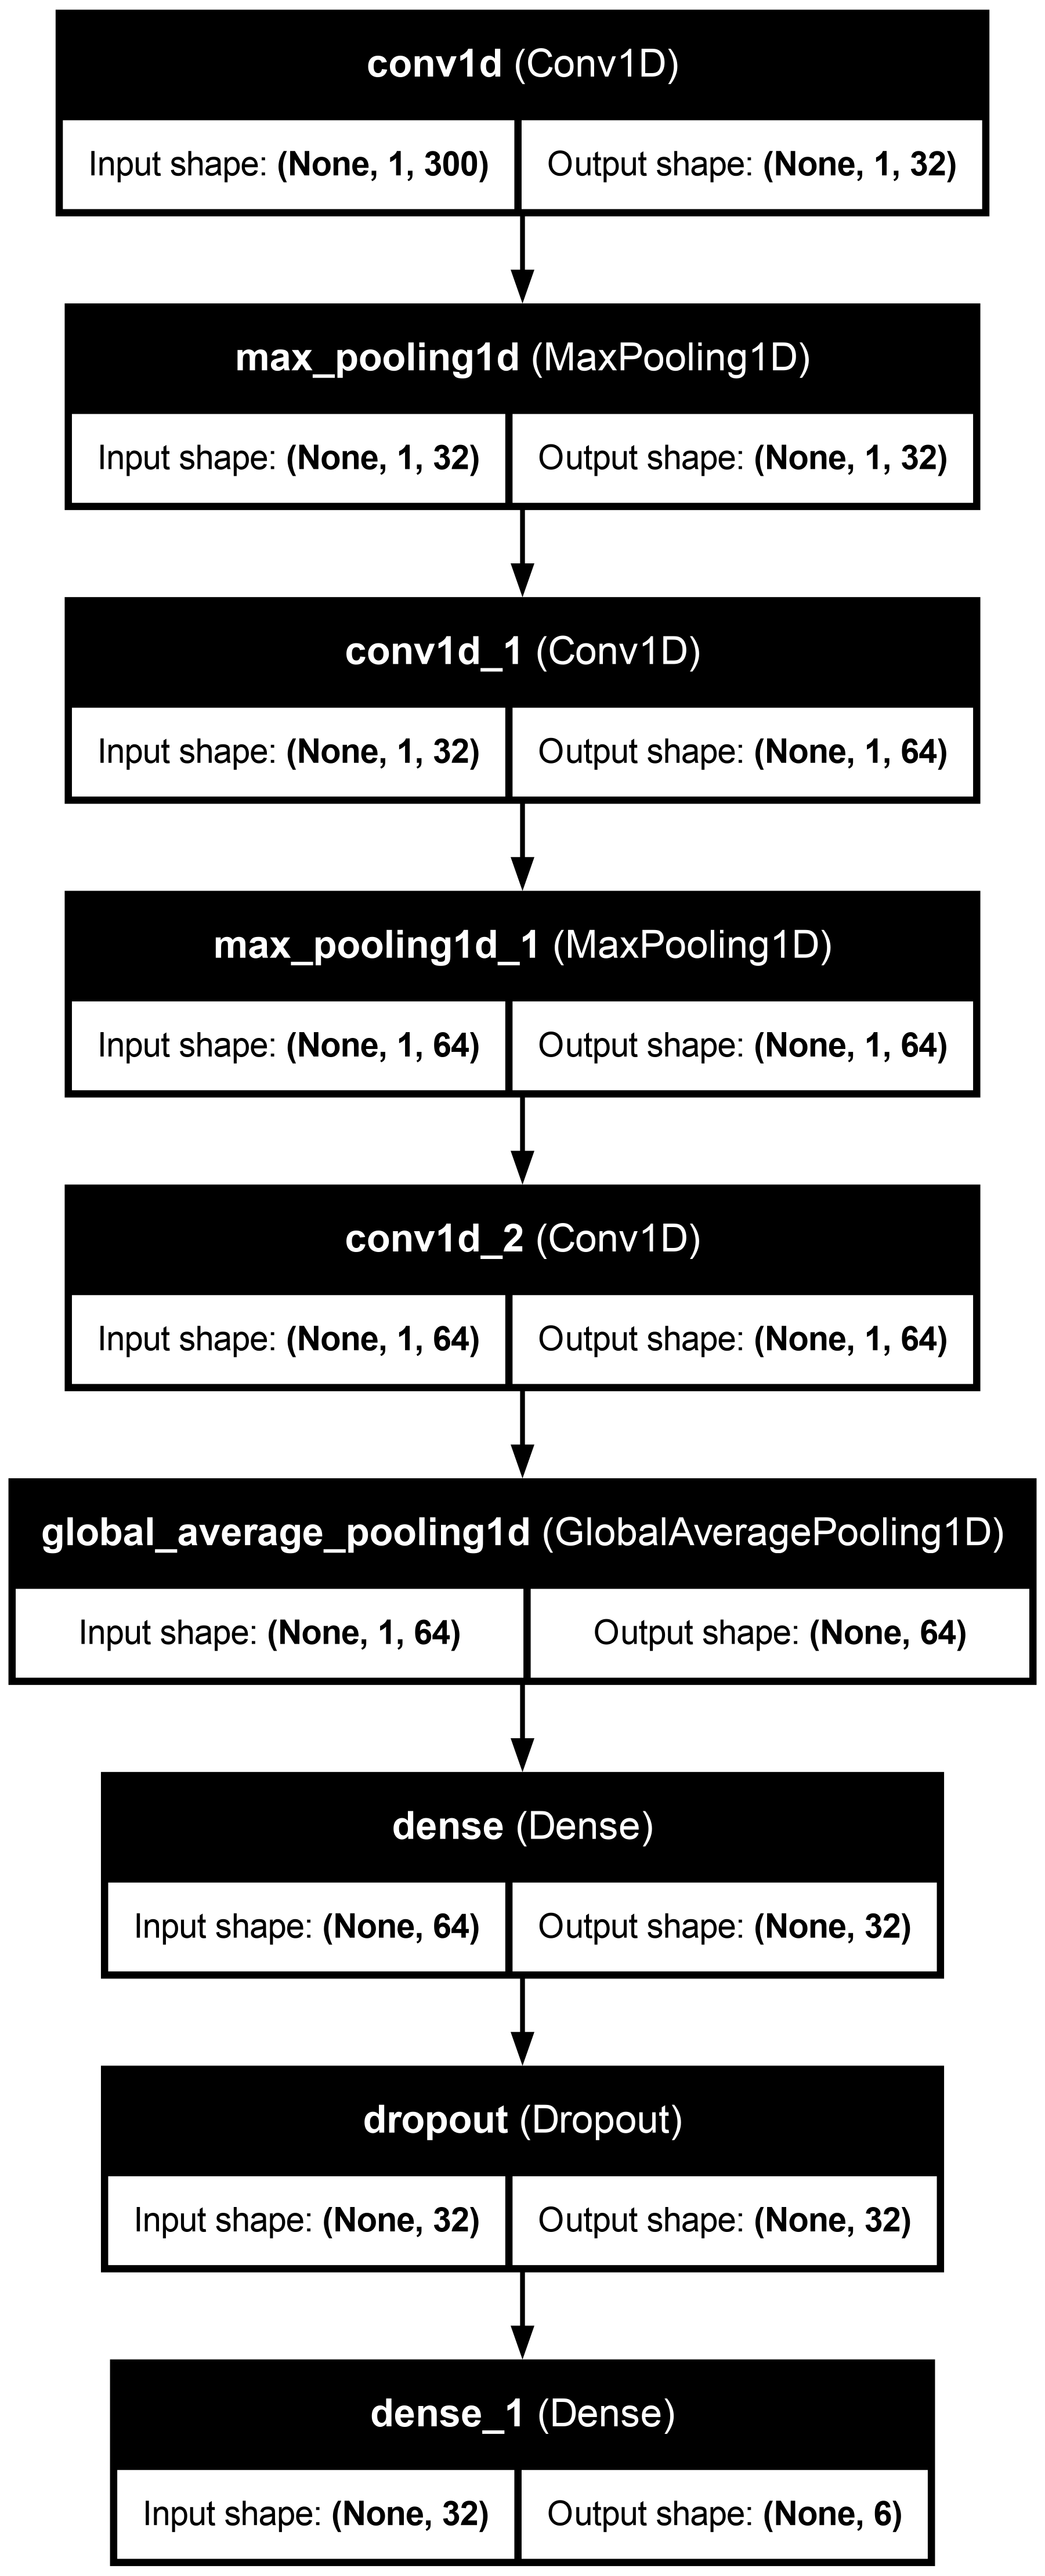
\includegraphics[width=0.3\textwidth]{Imagenes/Bitmap/best-cnn1.0.png}
    \caption{Esquema del modelo CNN}
    \label{fig:cnn-1.0-ejemplo}
\end{figure}

\begin{figure}[H]
    \centering
    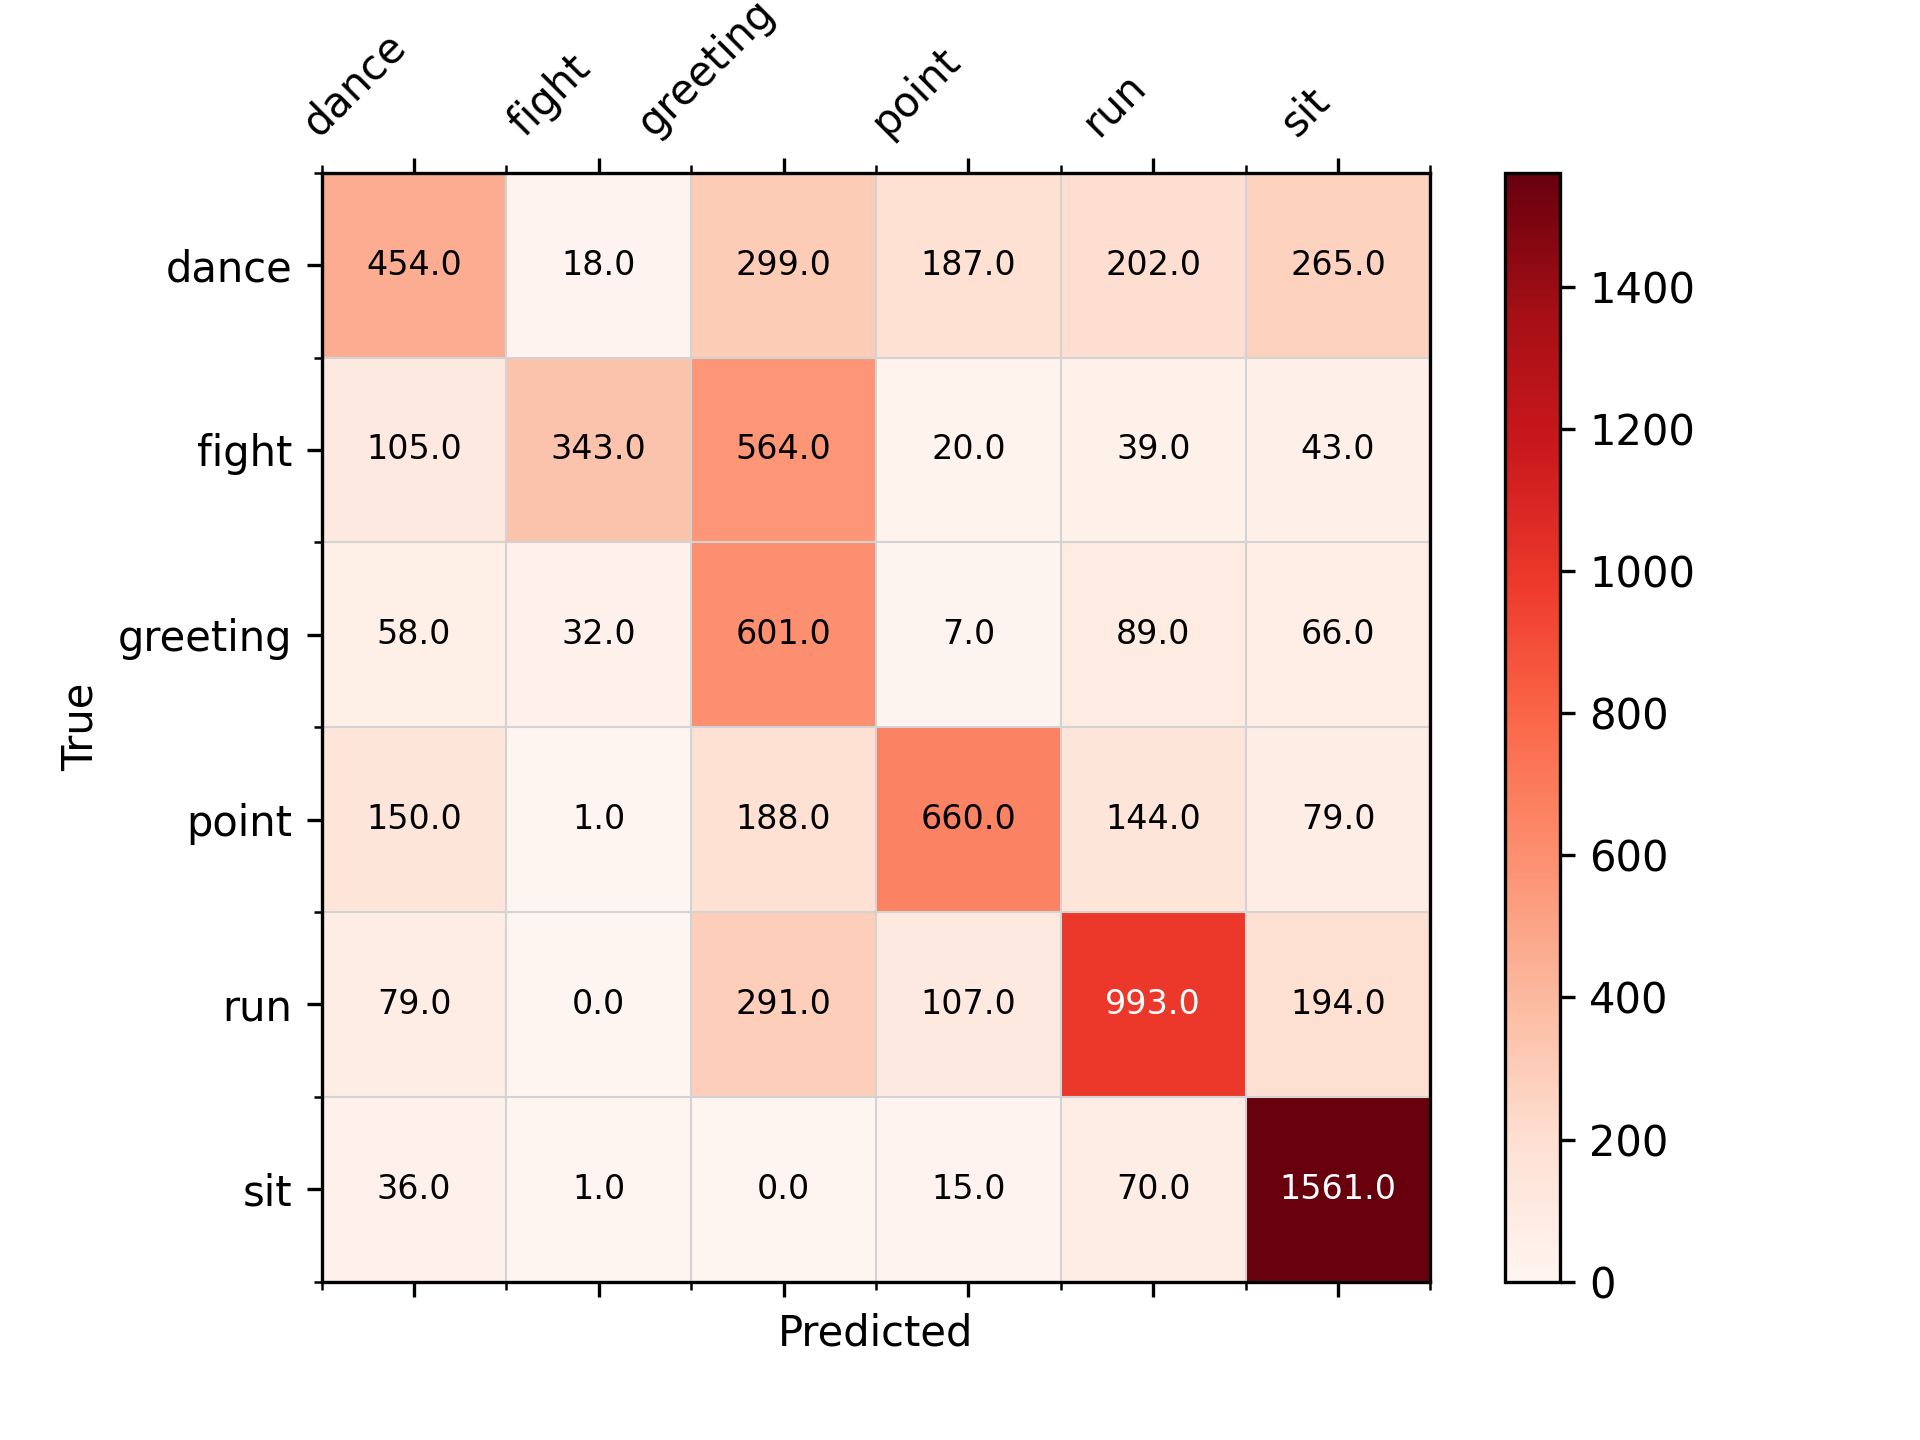
\includegraphics[width=0.6\textwidth]{Imagenes/Bitmap/CM_best-cnn1.0.png}
    \caption{Matriz de confusión del modelo CNN}
    \label{fig:cnn-1.0-matriz-ejemplo}
\end{figure}

\begin{figure}[H]
    \centering
    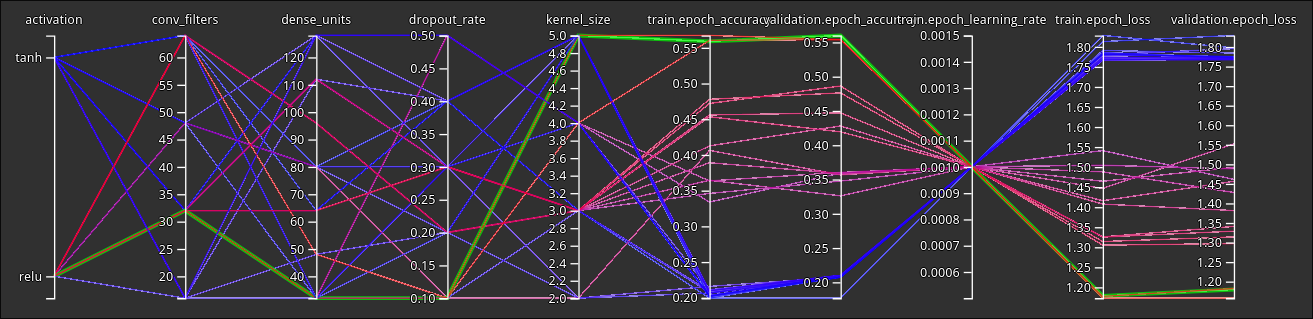
\includegraphics[width=0.8\textwidth]{Imagenes/Bitmap/tb-cnn-1.0.png}
    \caption{Gráfico de entrenamiento del modelo CNN}
    \label{fig:cnn-1.0-grafico-ejemplo}
\end{figure}

\subsubsection{\gls{rnn}}

Con el \gls{rnn} se sigue la misma base que para los dos modelos anteriores. La clase \textit{RNNTrainer} (estructura en la figura \ref{fig:rnn-estructura} )es muy similar a las anteriores, cambiando una vez más los hiperparámetros a buscar. En este caso son:

\begin{itemize}
    \item \textbf{activation}: Función de activación de la capa oculta.
    \item \textbf{activity regularizer}: Regularizador de la capa oculta.
    \item \textbf{bias constraint}: Restricción del \textit{bias} de la capa oculta.
    \item \textbf{bias initializer}: Inicializador del \textit{bias} de la capa oculta.
    \item \textbf{bias regularizer}: Regularizador del \textit{bias} de la capa oculta.
    \item \textbf{dropout}: Porcentaje de \textit{dropout} de la capa oculta.
    \item \textbf{kernel constraint}: Restricción del kernel de la capa oculta.
    \item \textbf{kernel initializer}: Inicializador del kernel de la capa oculta.
    \item \textbf{kernel regularizer}: Regularizador del kernel de la capa oculta.
    \item \textbf{recurrent constraint}: Restricción de la capa oculta.
    \item \textbf{recurrent dropout}: Porcentaje de \textit{dropout} de la capa oculta.
    \item \textbf{recurrent initializer}: Inicializador de la capa oculta.
    \item \textbf{recurrent regularizer}: Regularizador de la capa oculta.
    \item \textbf{unroll}: Si se usa el \textit{unroll} de la capa oculta.
    \item \textbf{use bias}: Si se usa el \textit{bias} de la capa oculta.
\end{itemize}

\begin{figure}[h!]
    \centering
    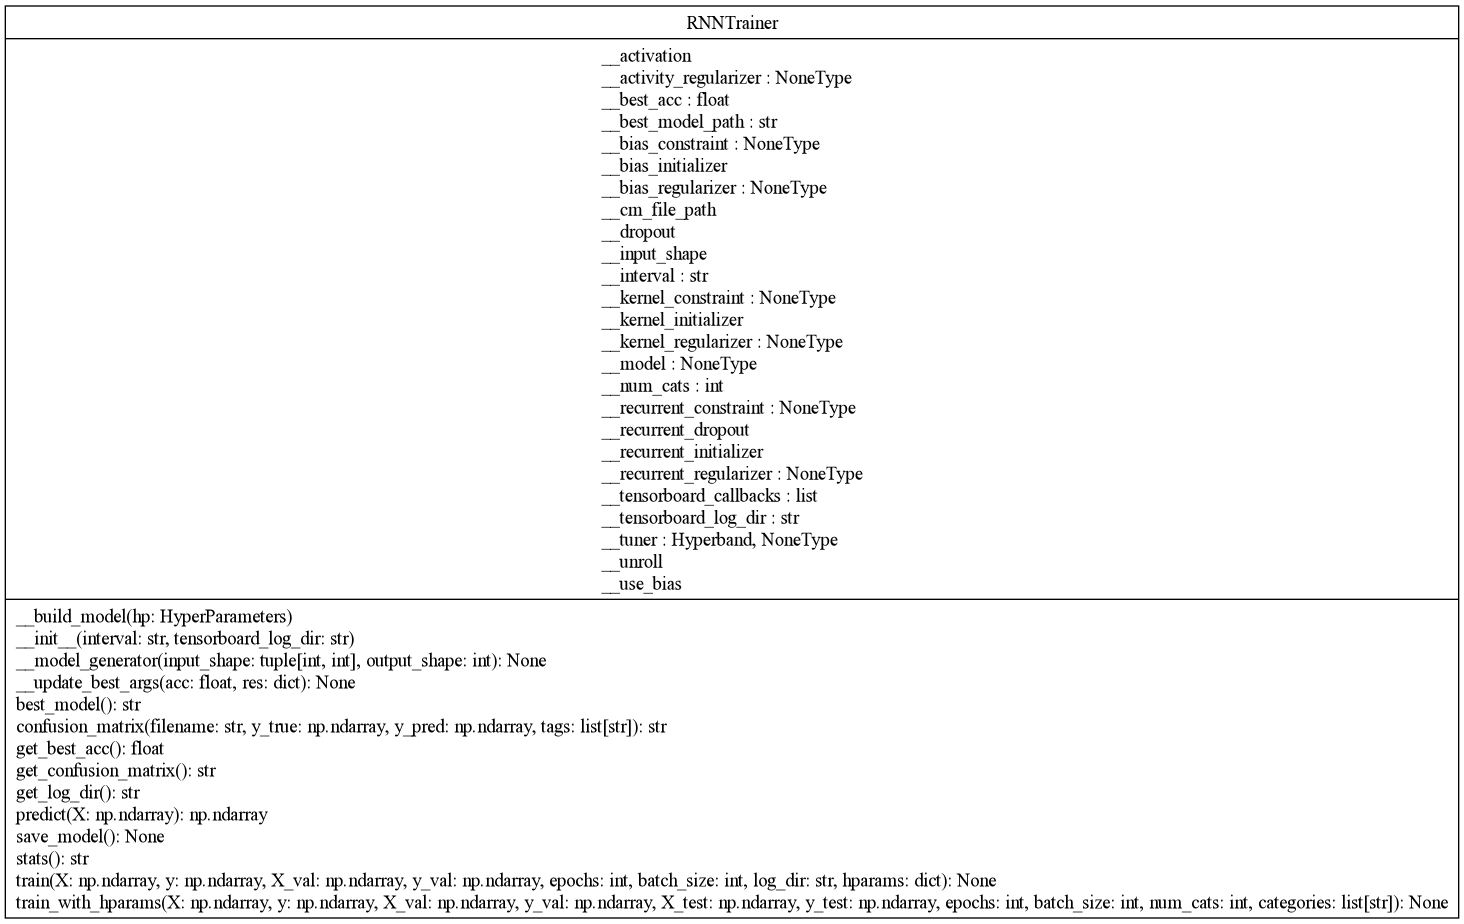
\includegraphics[width=0.8\textwidth]{Imagenes/Bitmap/classes_RNNTrainer.png}
    \caption{Estructura de la clase RNNTrainer}
    \label{fig:rnn-estructura}
\end{figure}

A pesar de ser el modelo con mayor busqueda de hiperparámetros, está en una reñida competición con el modelo \gls{cnn} para ver cual de los dos detecta peor los gestos. Su mejor intervalo ha sido el de 0.8 segundos con una precisión de 0.42714 en entrenamiento y 0.47865 en validación. En la figura \ref{fig:rnn-0.8-ejemplo} se puede ver el esquema del modelo, en la figura \ref{fig:rnn-0.8-matriz-ejemplo} la matriz de confusión y en la figura \ref{fig:rnn-0.8-grafico-ejemplo} el gráfico de entrenamiento. En este caso podemos ver que los gestos que peor detecta son baile y saludo (siendo pelea muy confundida con saludo). Los resultados del resto de intervalos se pueden ver en el apéndice \ref{appendix:resultadosRNN}.

\begin{figure}[H]
    \centering
    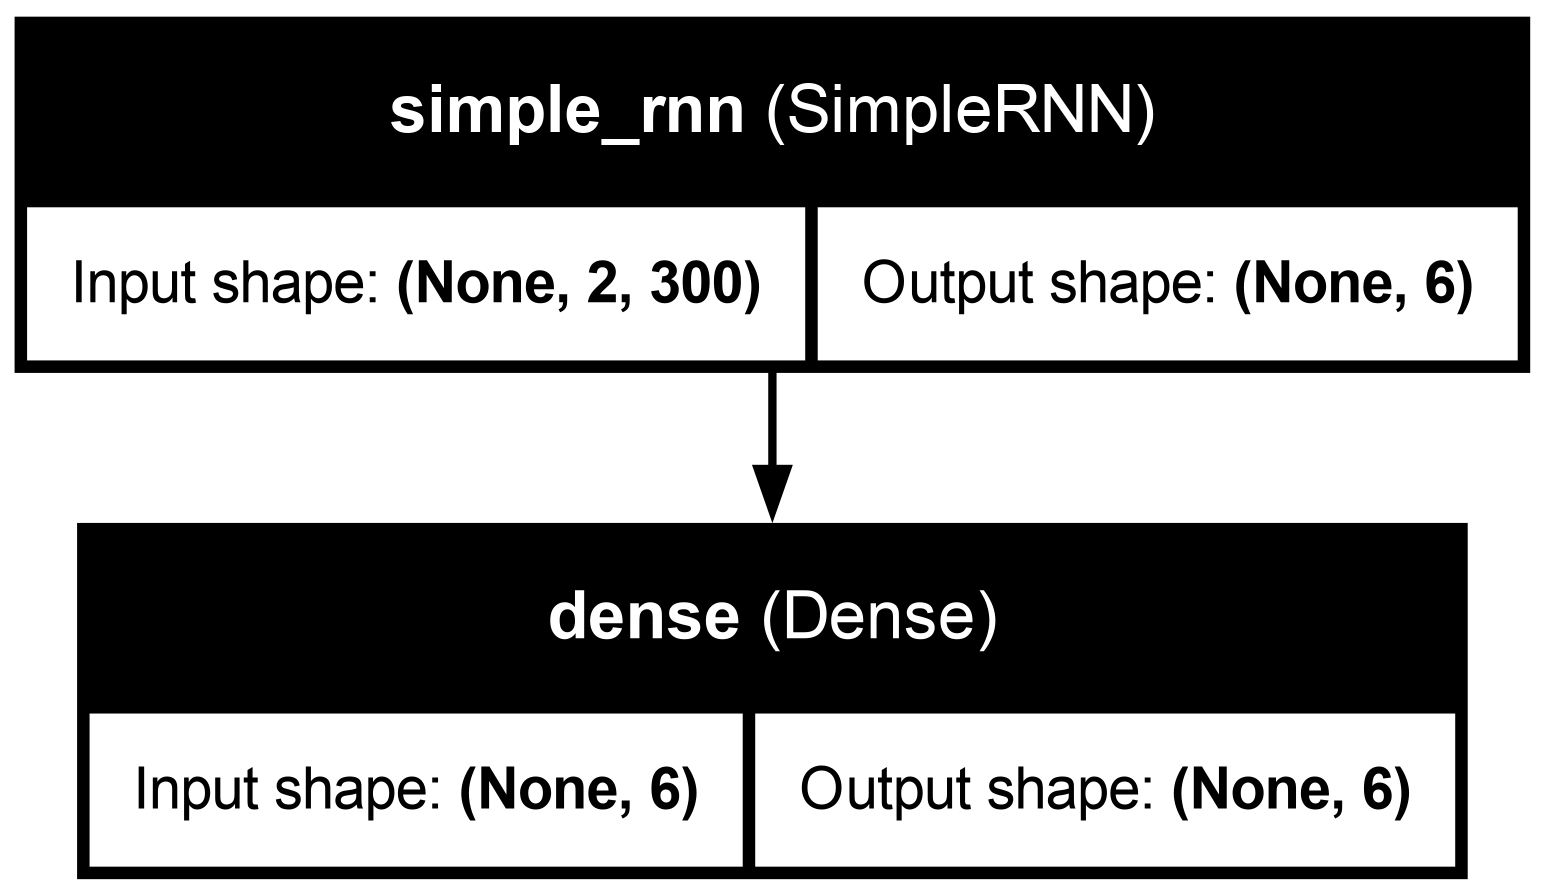
\includegraphics[width=0.3\textwidth]{Imagenes/Bitmap/best-rnn0.8.png}
    \caption{Esquema del modelo RNN}
    \label{fig:rnn-0.8-ejemplo}
\end{figure}

\begin{figure}[H]
    \centering
    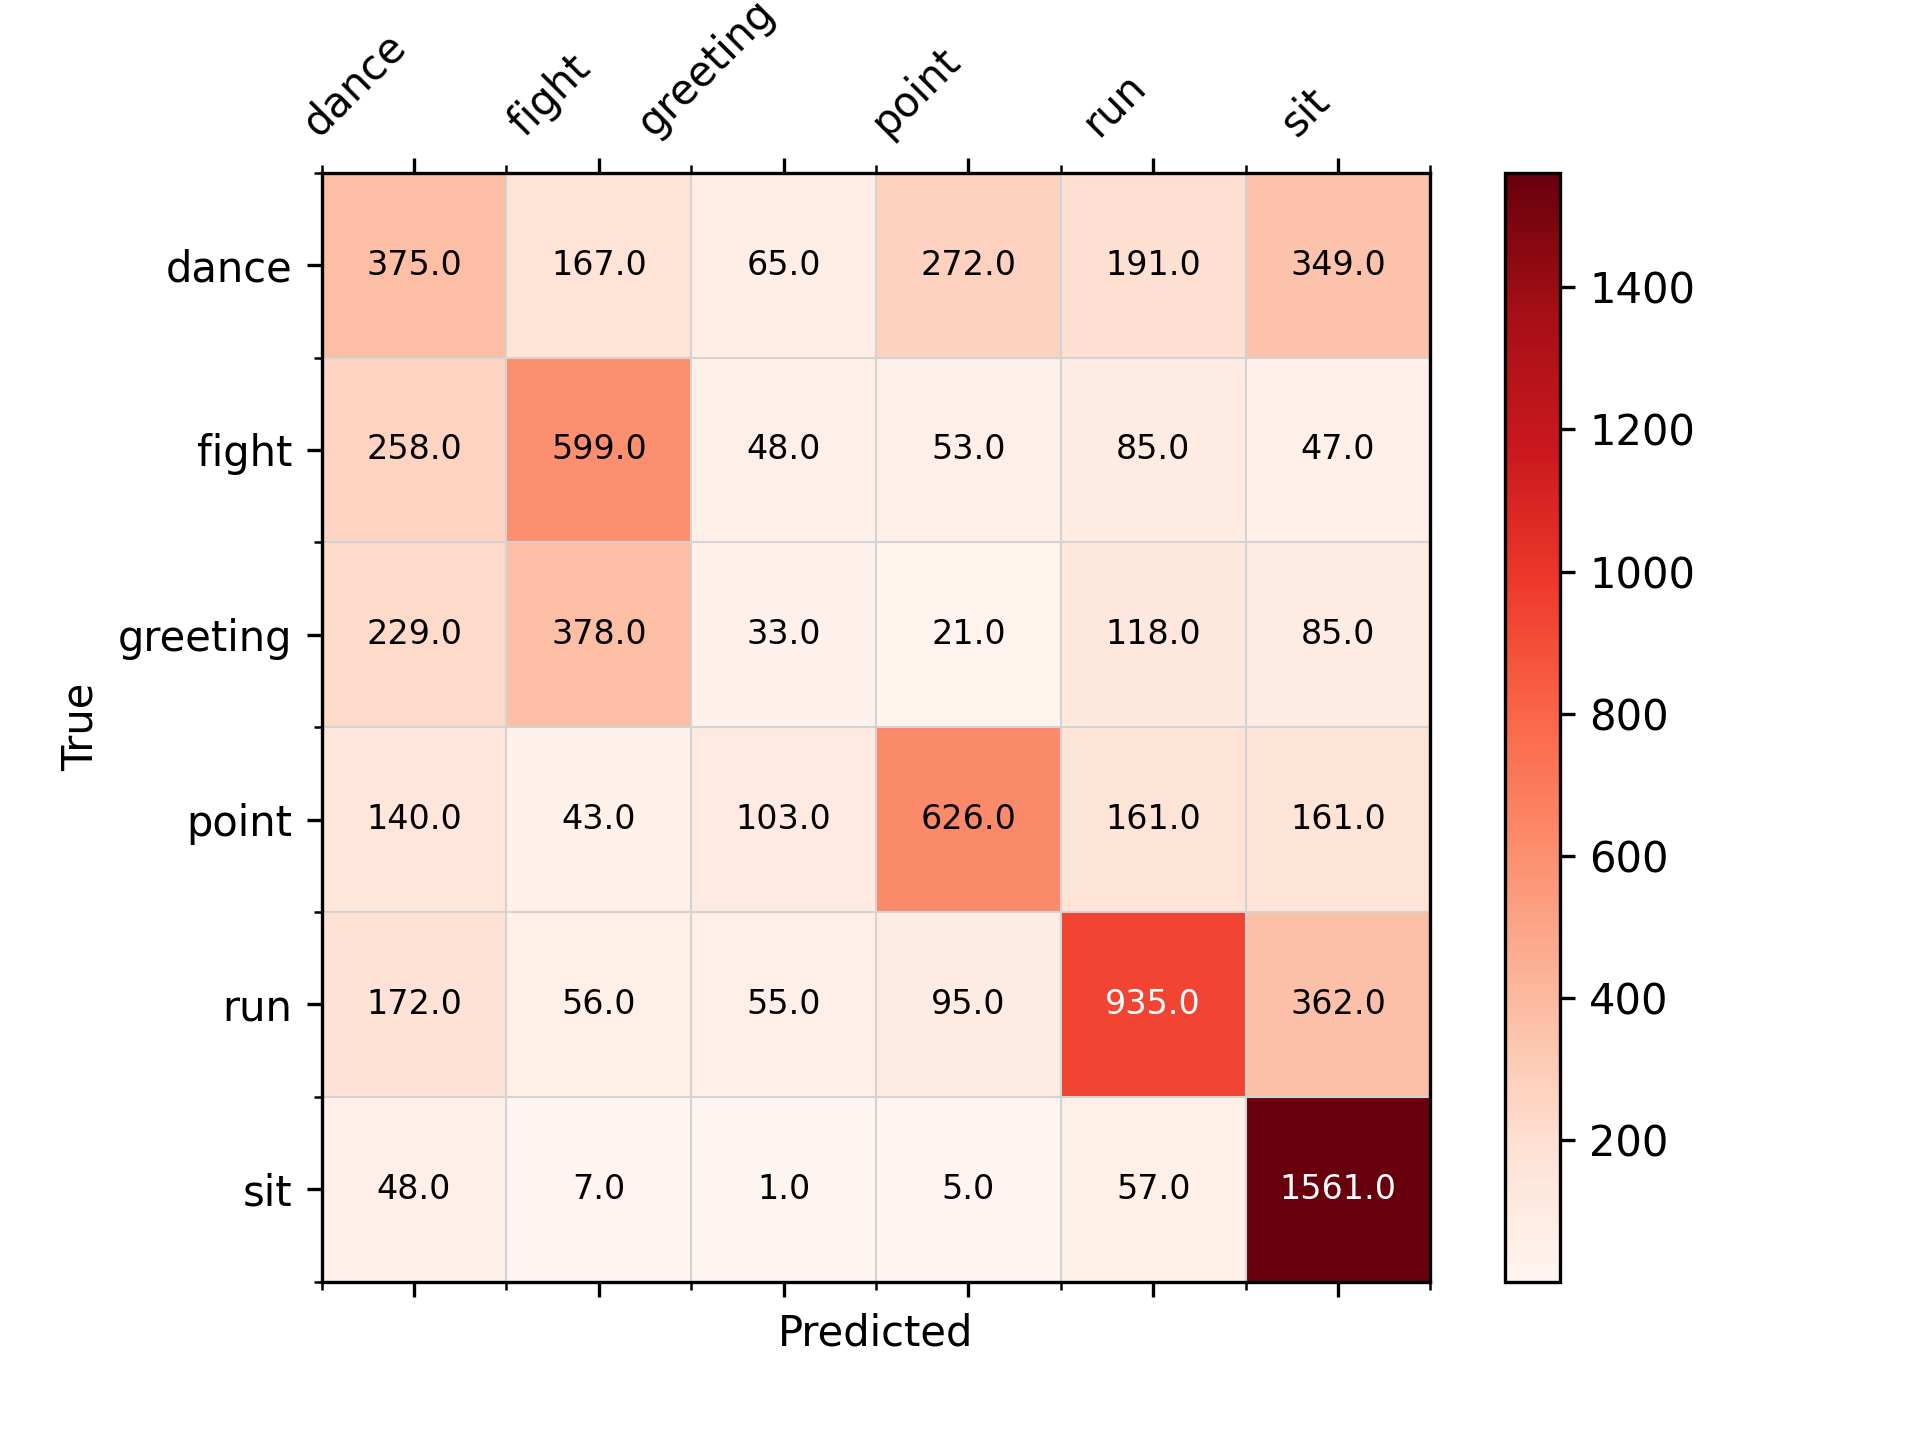
\includegraphics[width=0.6\textwidth]{Imagenes/Bitmap/CM_best-rnn0.8.png}
    \caption{Matriz de confusión del modelo RNN}
    \label{fig:rnn-0.8-matriz-ejemplo}
\end{figure}

\begin{figure}[H]
    \centering
    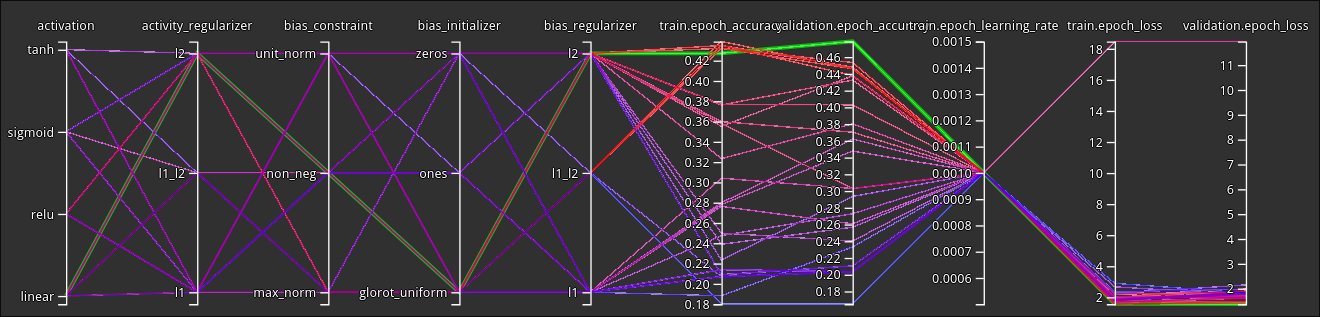
\includegraphics[width=0.8\textwidth]{Imagenes/Bitmap/tb-rnn-0.8.png}
    \caption{Gráfico de entrenamiento del modelo RNN}
    \label{fig:rnn-0.8-grafico-ejemplo}
\end{figure}

\subsubsection{\gls{randomforest}}

El entrenador del \gls{randomforest} es el más sencillo y el más distinto de todos. Este modelo no es una red neuronal, sino un modelo clásico de clasificación. La clase \textit{RandomForestTrainer} (estructura en la figura \ref{fig:rf-estructura}) sigue utilizando la función train\_with\_hparams como las anteriores aún no habiendo hparams como tal, haciendo esto se consigue mantener la igualdad de todas las clases de cara a la interfaz de gradio.

Este modelo no usa tensorflow como tal, dado que YDF es un desarrollo que deja atrás el uso de TensorFlow Decision Forest para implementar algoritmos más eficientes tanto en entrenamiento como en inferencia. A pesar de ser un desarrollo paralelo, el equipo de YDF decide hacer el modelo compatible con Tensorflow para poder integrarlo en un mayor ecosistema. Estos datos de mayor eficiencia se pueden comprobar en el estudio \cite{GBBSP23}.

A diferencia de los modelos anteriores, este modelo usa DataFrames de pandas para el entrenamiento y la predicción en vez de tensores. En este entrenamiento usamos \textit{RandomSearchTuner} para buscar la mejor combinación de número de árboles, profundidad máxima y mínimo de ejemplos.

\begin{figure}[h!]
    \centering
    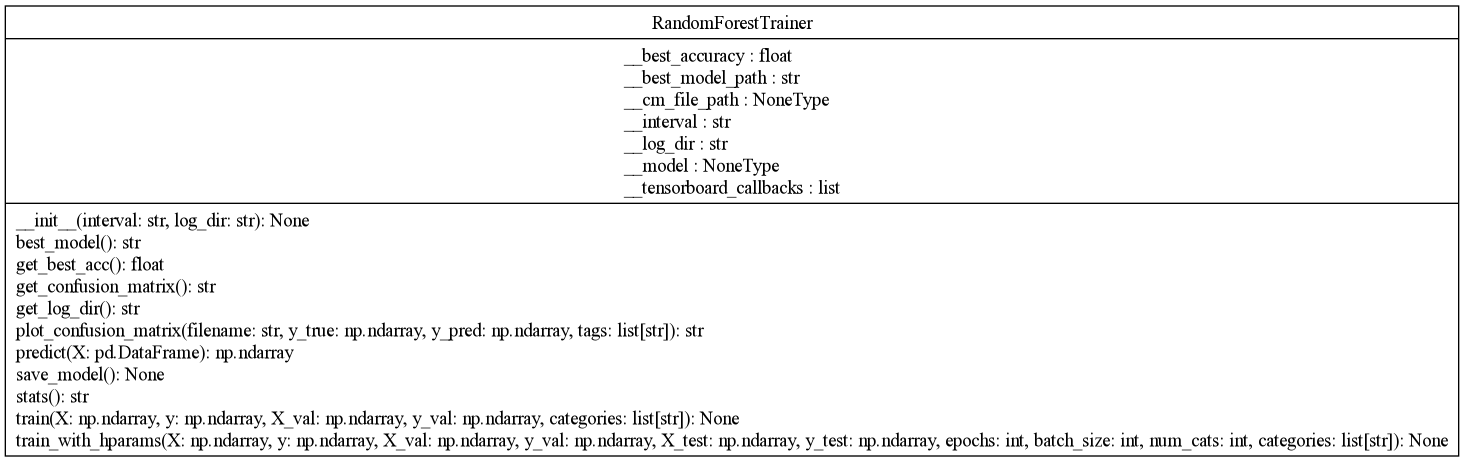
\includegraphics[width=0.8\textwidth]{Imagenes/Bitmap/classes_RandomForestTrainer.png}
    \caption{Estructura de la clase RFTrainer}
    \label{fig:rf-estructura}
\end{figure}

Por desgracia, este modelo no deja una constancia tan rigurosa como los anteriores dado que no usa TensorBoard ni tiene un equivalente. A pesar de esto, este es el modelo con mayor rendimiento de lejos. Todos los intervalos tienen un rendimiento más o menos equivalente, ganando el de 0.8 segundos por muy poco.

En la figura \ref{fig:rf-0.8-matriz-ejemplo} se puede ver la matriz de confusión del modelo y en el apendice \ref{appendix:resultadosRF} se pueden ver los resultados de todos los intervalos. En este caso podemos ver que los gestos que peor detecta son pelea y saludo. La precisión en validación fue de 0.85936 y de 0.97487 en entrenamiento, lo que lo convierte en el mejor modelo entrenado.

\begin{figure}[H]
    \centering
    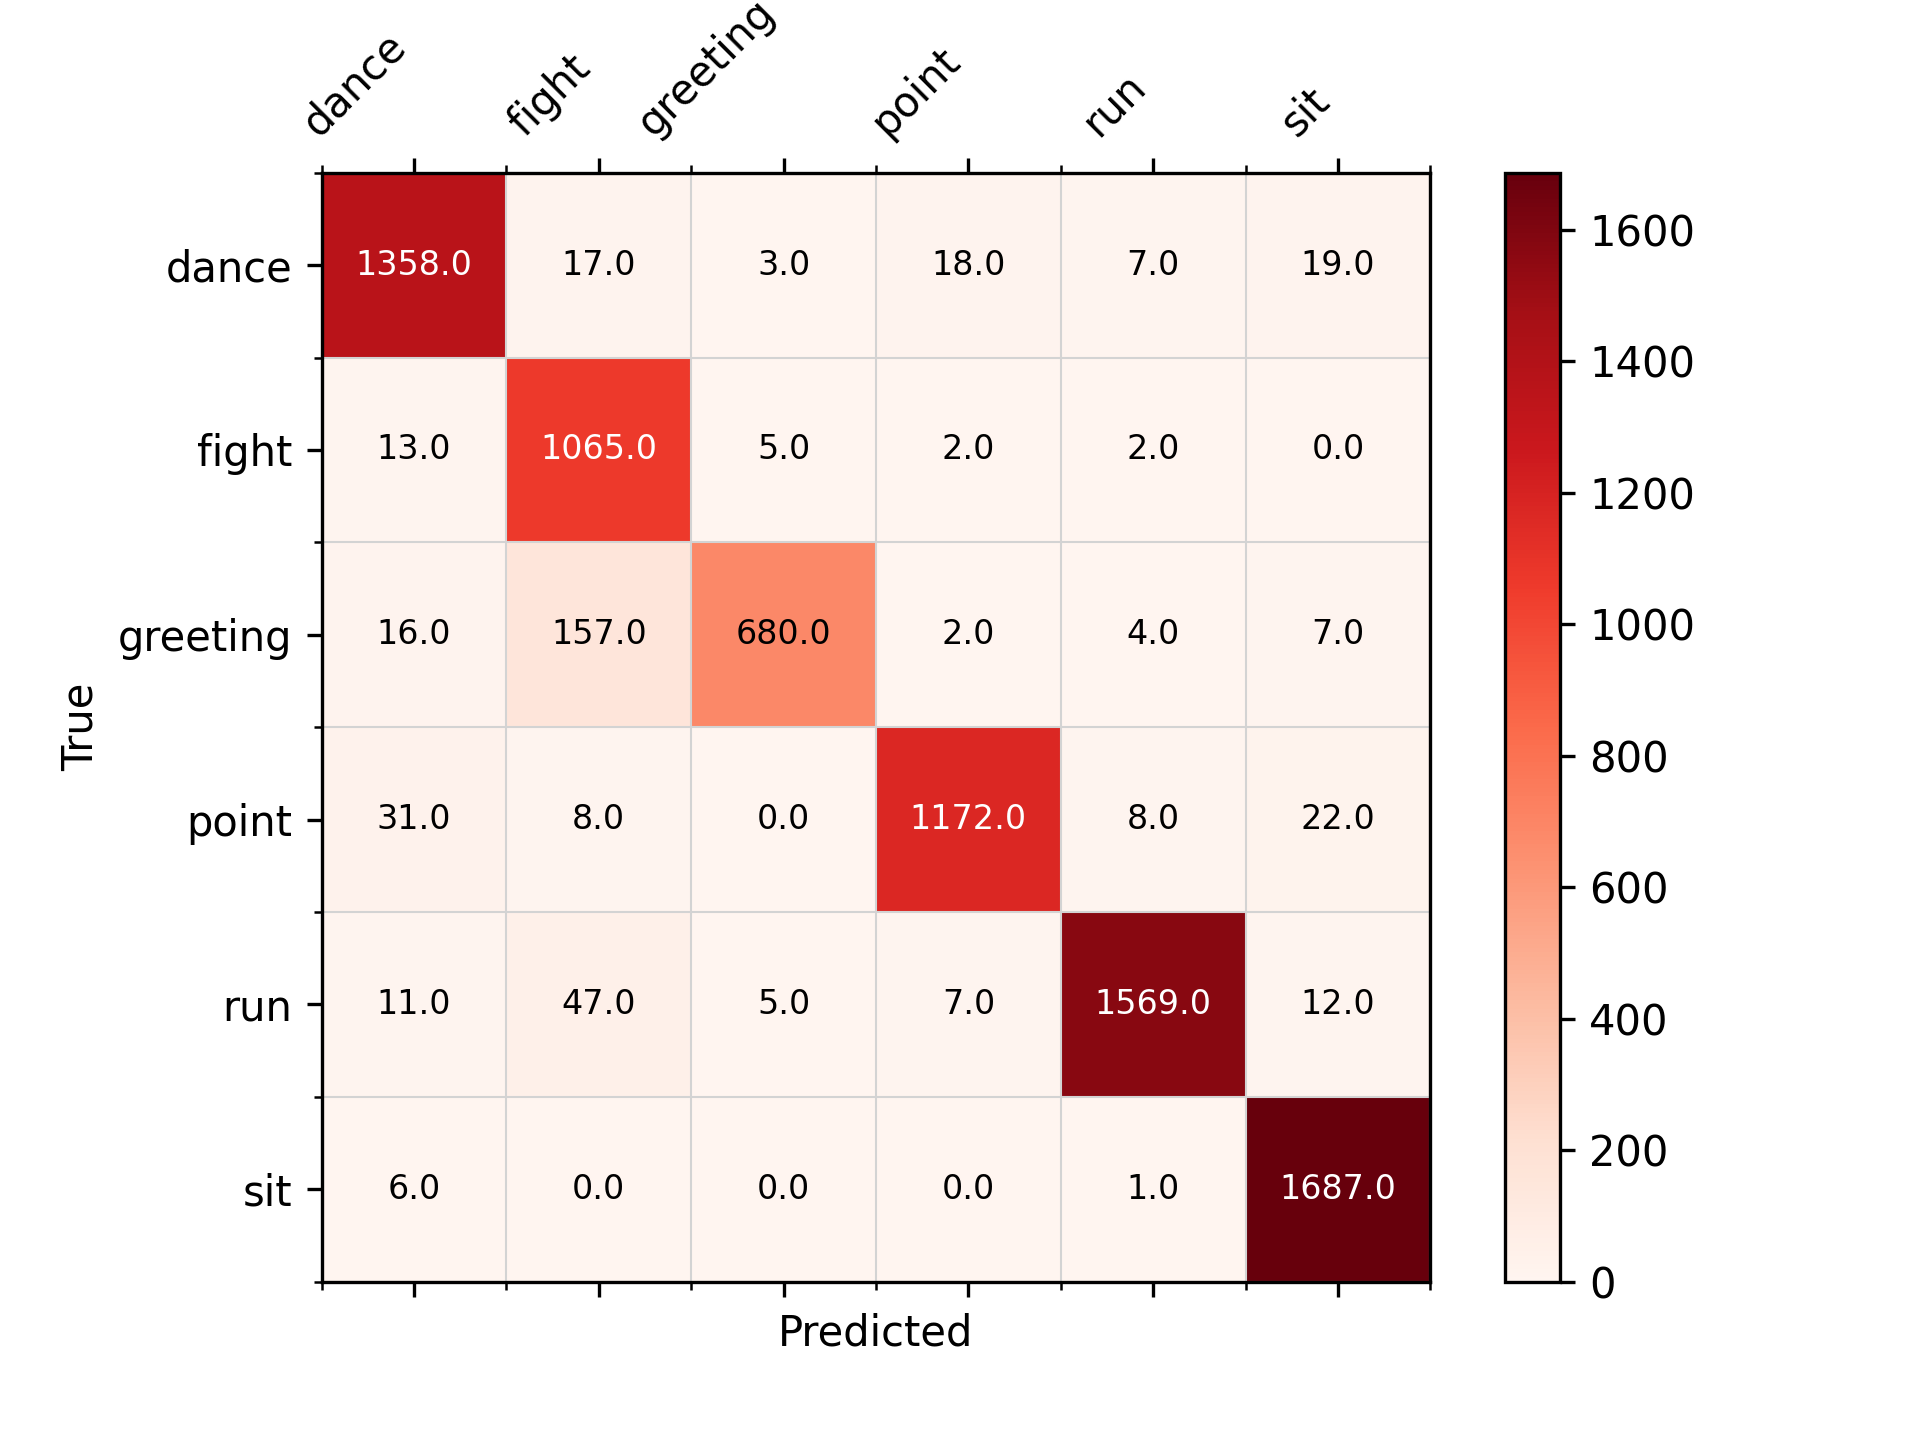
\includegraphics[width=0.6\textwidth]{Imagenes/Bitmap/CM_best_rf_0.8.png}
    \caption{Matriz de confusión del modelo RandomForest}
    \label{fig:rf-0.8-matriz-ejemplo}
\end{figure}

Este modelo finalmente es exportable a TensorFlow, siendo esto muy útil para su desplegado y compatibilización con otras herramientas. Dentro del repo, en la carpeta de ``notebooks'' se puede ver un resumen de las características más decisivas del modelo y su importancia en la diferenciación de dos gestos cuales sean.

\subsection{TensorFlow Serving}

Que todos los modelos sean exportables a TensorFlow permite el uso de TensorFlow Serving (\cite{olston2017tensorflowservingflexiblehighperformanceml}) para desplegar modelos. Serving nos proporciona una interfaz sencilla mediante \gls{API REST} para re entrenar los modelos y poder hacer inferencia sobre ellos desde cualquier máquina conectada a la red.

Este método de desplegado es especialmente útil a la hora de integrar los modelos con otras tecnologías sin necesidad de hace traducciones a otros lenguajes o formatos. El servidor se despliega usando docker y cogiendo el modelo de la última \textit{release} del repositorio. Para hacer una inferencia solo hay que hacer una petición \textit{POST} con el formato visto en la figura \ref{fig:ejemplo-petición} y el servidor devuelve la respuesta vista en la figura \ref{fig:ejemplo-respuesta}.

\begin{figure}[H]
    \centering
    \begin{lstlisting}[style=custombash]
curl <model_server>/v1/models/<model_name>:predict \
-X POST \
-d '{"instances": [{
    "feature_0":0.24,
    "feature_1":0.12,
    ... 
    "feature_599":0.56
}]}'
    \end{lstlisting}
    \caption{Ejemplo de petición a TensorFlow Serving}
    \label{fig:ejemplo-petición}
\end{figure}

\begin{figure}[H]
    \centering
    \begin{lstlisting}[style=custombash]
{
    "predictions": [{
        "scores": [0.981395662, 0.0186043456, 0.1920000, 0.0112349, 0.0001234, 0.0001234],
         "classes": ["dance", "fight", "greeting", "point", "run", "sit"]
    }]
}
    \end{lstlisting}
    \caption{Ejemplo de respuesta de TensorFlow Serving}
    \label{fig:ejemplo-respuesta}
\end{figure}

En el repositorio se pueden encontrar dos scripts, uno para windows y otro para linux, que permiten desplegar el servidor de manera automática siempre que docker ya esté instalado en el sistema.

\subsection{Hardware, complejidad de datos y otras limitaciones}

Este estudio ha estado muy limitado por el hardware disponible para el mismo. El equipo usado para el modelo tenía gráficas de consumidor de hace más de 5 años, haciendo que los modelos con redes neuronales tardaran bastante en entrenarse. Esto no fue un problema en el caso del \gls{randomforest}, ya que se entrena en \gls{cpu} y permite unos tiempos de entrenamiento mucho menores.

Estas limitaciones de hardware también han afectado a la visión de los modelos a desarrollar, ya que en un principio se pensó en hacer modelos lo más simples posibles para poder utilizarlos incluso en equipos más limitados (gafas de \gls{vr} o equipos más antiguos).

Así mismo, la falta de espacios y de tiempo han resultado en que, junto a la falta de datasets ya formados, el número de datos fuera limitado para lo que requeriría el entrenamiento de redes neuronales.
\section{Aplicación final}
\label{sec:aplicacionFinal}
%\include{Capitulos/Capitulo4}
%\include{Capitulos/Capitulo5}
\chapter{Conclusiones y Trabajo Futuro}
\label{cap:conclusiones}

\section{Conclusiones}

El objetivo de este estudio era la creación de un modelo de \gls{ia} que pudiera detectar una serie de gestos de usuarios con un traje de captura de movimiento. Para ello, se buscaron datasets de gestos que concordaran con las restricciones del trabajo. Al no encontrar nada fácilmente adaptable o con los gestos necesitados, se creó un dataset de animaciones, con datos tanto generados por ordenador como recopilados de usuarios reales.

Las animaciones generadas por ordenador se convirtieron a \gls{csv} por una herramienta creada por los autores del trabajo, al igual que las recolectadas por usuarios reales se hicieron con otra herramienta de los mismos creadores.

Tras los entrenamientos de los distintos modelos de \gls{ia}, se llegó a la conclusión de que el \gls{randomforest} es el mejor modelo por diferentes razones. Tras esto, se creó una aplicación a modo de demostración para mostrar el resultado final.

Las conclusiones de cada una de las partes del trabajo se presentan en las siguientes secciones de manera más detalladas.

\subsection{Conclusiones de la búsqueda de datasets}
Tras la búsqueda de datasets de animaciones se ha llegado a la conclusión de que no existen datasets públicos suficientes para el objetivo de este estudio.

Estas conclusiones nos llevaron a la necesidad de crear un dataset propio recabando animaciones de bancos de animaciones y mediante pruebas con usuarios.

\subsection{Conclusiones de la extracción de animaciones de bancos de animaciones}
Para la conversión de animaciones de Mixamo se ha creado una herramienta para hacerlo de forma automática y se ha modificado otra herramienta para hacer una descarga en masa de estas animaciones.

La herramienta de conversión de gestos cumple su objetivo completamente, ya que tan solo indicando el nombre de la carpeta que contiene los gestos descargados coge los gestos, se procesan en Unity y se suben a Kaggle de forma automática.
Además la herramienta es independiente al número de gestos que se quieren convertir y a su vez del número de animaciones que hay de esos gestos, consiguiendo una gran escabilidad de esta forma haciendo posible la introducción de nuevos gestos sin tener que cambiar nada de la herramienta.

\subsection{Conclusiones de la recolección de animaciones con usuarios}
Para la recolección de datos con usuarios se anunció de forma insistente en las redes sociales de los autores del estudio así como por las distintas facultades de la Universidad Complutense de Madrid.
Los anuncios cumplieron su objetivo, consiguiendo 75 respuestas de los cuales se presentaron 65 participantes, consiguiendo un 86,67\% de asistencia.

Como se puede ver en las figuras del apéndice \ref{appendix:formularioDemografia} el grupo de participantes, con excepción del género no binario, es heterogéneo en cuanto al género con una pequeña diferencia de porcentaje entre hombres y mujeres.
Donde se puede ver mayor diferencia es entre la mano dominante de los usuarios, siendo los zurdos tan solo un 6.15\% de la población total del grupo.

Gracias a la prueba se obtuvieron 975 animaciones (195 animaciones de saludar, señalar, sentarse, pelear y correr).

\subsection{Conclusiones de la comparativa entre los modelos de \gls{ia}}

En cuanto a los modelos de \gls{ia}, se ha visto que los modelos de redes neuronales no han obtenido los resultados esperados, siendo esto seguramente por una mezcla de falta de datos y simplificación de las redes neuronales para asegurar un tiempo de entrenamiento menor y un computo más rápido a la hora de realizar inferencias.

Sin embargo, el \gls{randomforest} ha sido el que ha obtenido mejores resultados, siendo el modelo más rápido (tanto en inferencia como en entrenamiento), el modelo más ligero y el modelo más adaptable. Este modelo se podría usar en sistemas con recursos limitados como pueden ser gafas de \gls{vr} independientes como las Meta Quest o en ordenadores más potentes, e incluso en ecosistemas de \gls{ia} por su posible traducción a TensorFlow ya implementada.

En el análisis de los resultados del \gls{randomforest} se ha visto que el modelo le da una gran importancia a la coordenada y de la pierna izquierda, a la coordenada y del pie izquierdo en el segundo intervalo de tiempo. Esto puede indicar que los gestos dependen mucho de la posición de las piernas para discriminar si se está corriendo, bailando, saludando o señalando.

También se puede ver una ligera confusión entre los gestos de pelea y saludar. Esto puede ser debido a los movimientos rápidos de las manos en ambos tipos de gesto, que al no tener dedos por limitación del traje, puede dar lugar a confusión entre un puñetazo y un saludo.

\subsection{Conclusiones de la aplicación final}
La aplicación final es una demo que se conecta a un servidor para mostrar los resultados.

La parte negativa de esta aplicación es la forma de conectarse con el servidor en el que está el modelo, ya que hace peticiones web al servidor de Tensor Serving directamente, lo que lo hace dependiente de éste.

Finalmente la aplicación final cumple su propósito de enseñar al usuario la animación predicha con una latencia mínima.


\subsection{Limitaciones}

Este estudio ha tenido una serie de limitaciones, desde escasez de datasets públicos, desbalanceo de tipos de animaciones, falta de más datos de usuarios reales, problemas de entrenamiento con los modelos de redes neuronales y problemas de falta de datos para estos mismos modelos.

La limitación de escasez de datasets se debe no solo a la falta en número de datasets, sino también a la falta de gestos referentes a comunicación no verbal, habiendo algunos sobre deportes o temáticas muy concretas y pocos de carácter general.  Otra limitación de estos datasets ha sido la facilidad de adecuación o conversión a un formato compatible con el traje de captura de movimiento usado en el estudio.

En cuanto al desbalanceo de los tipos de animaciones, la problemática viene dada por la duración de las animaciones de baile de Mixamo. Al seguir el proceso de estandarizado, las distintas animaciones de baile se multiplican en un número bastante mayor que los del resto de tipos. Esto no se solucionó con los datos recopilados de usuarios reales, ya que aún que se obtuvo un gran número de animaciones nuevas, tras la estandarización las de baile seguían prevaleciendo por bastante. Esto se puede ver en las figuras \ref{fig:datos-bruto} y \ref{fig:datos-estandar}.

Los modelos de redes neuronales no han dado los resultados esperados, esto puede ser por la falta de datos, que aunque haya un número que a simple vista parece suficiente no lo es para entrenar redes neuronales, por las limitaciones de hardware para entrenar modelos más complejos y por los tiempos requeridos para la realización de este estudio no ser lo suficientemente largos como para llevar a cabo entrenamientos más extensos y con mayor búsqueda de hiperparámetros.

Todas estas limitaciones, han llevado al siguiente plan de trabajo a futuro.


\section{Trabajo Futuro}

El trabajo a futuro de este estudio se puede centrar en varios esfuerzos:
\begin{itemize}
    \item Mejorar el dataset, incluyendo gente con diversidad funcional, aumentando el número de muestras por gesto, teniendo en cuenta los dedos de las manos y añadiendo nuevas categorías. Esto no solo puede llegar a mejorar el rendimiento de modelos de redes neuronales, sino que puede dotar de mayores diferencias a los modelos para poder generalizar mejor.
    \item Investigar otros modelos de \gls{ia} que puedan mejorar la precisión de la clasificación y hacer clasificación no solo de gestos, sino también de emociones. Esto podría ayudar a que los \glspl{npc} puedan reaccionar de una manera más natural a los gestos del usuario, haciendo la interacción más inmersiva.
    \item Estandarizar el servidor para que pueda ser usado con otras tecnologías de \gls{ia} y no solo con TensorFlow. Esto permitiría integrar tecnologías que vayan surgiendo en el futuro a aplicaciones ya existentes.
    \item Implementar otro modelo que no solo tenga en cuenta el gesto predicho actual sino también todo el contexto para poder avanzar en el uso de la comunicación no verbal con \glspl{npc}.
    \item Evaluación del resultado final con usuarios.
\end{itemize}





%%%%%%%%%%%%%%%%%%%%%%%%%%%%%%%%%%%%%%%%%%%%%%%%%%%%%%%%%%%%%%%%%%%%%%%%%%%
% Si el TFG se escribe en inglés, comentar las siguientes líneas 
% porque no es necesario incluir nuevamente las Conclusiones en inglés
\begin{otherlanguage}{english}
  \chapter*{Introduction}
\label{cap:introduction}
\addcontentsline{toc}{chapter}{Introduction}

\chapterquote{La revolución industrial y sus consecuencias han sido un desastre para la raza humana}{Theodore Kaczynski}

In recent years, there has been a great interest and evolution of virtual reality technologies led by companies such as Apple with the launch of Apple Glasses or Meta with the launch of Meta Quest 3 or its interest in the \gls{metaverse} with its application ``Meta Horizon Worlds''.


It is for this reason that it is interesting to investigate non-verbal communication in virtual environments, not only for applications with multiple users but also to improve interactions with \glspl{npc} in these types of environments.


The proposal in this Bachelor's Thesis is a first approach to how we can use Artificial Intelligence and motion capture technology to achieve this improvement in interactions in virtual worlds through non-verbal communication, being our case the exploration of the ability to classify different gestures.
The gestures we have focused on are six gestures that we have considered useful for an NPC to recognize in a video game. These gestures are:
\begin{enumerate}
	%\renewcommand{\theenumi}{\alph{enumi}}
	\item Dance
	\item Greet
	\item Point
	\item Sit down
	\item Fight
	\item Run
\end{enumerate}

To carry out this work, we have used the Meta (formerly Oculus) Quest 2 and 3 virtual reality glasses and the Perception Neuron 3 motion capture suit, from the company Noitom, as hardware and Python, C\# and Unity as the software requirements.
\section{Motivation}
Research on gesture recognition using \gls{ai} for possible implementations in the study and improvement of non-verbal communication in virtual environments.

\section{Objectives}
Implementation of an \gls{ai} model that, with low latency, allows identifying the gesture being performed with a motion capture suit.

\section{Work Plan}
The Work Plan consists of several steps:

\begin{enumerate}
	%\renewcommand{\theenumi}{\alph{enumi}}
	\item Search for a dataset: generate a dataset large enough with several examples of gestures to adequately train different models.
	\item Implementation of \gls{ai} models: implementation of several \gls{ai} models to make a comparison between them and decide which one is the most suitable considering its prediction speed and accuracy.
	\item Development of a final application: development of an application for the Meta Quest as a demo that connects to the chosen model and allows real-time usage.
\end{enumerate}










  \chapter*{Conclusions and Future Work}
\label{cap:conclusions}
\addcontentsline{toc}{chapter}{Conclusions and Future Work}
\section{Conclusions}

The objective of this study was to create an \gls{ai} model capable of detecting a series of gestures from users wearing a motion capture suit. To achieve this, datasets of gestures that matched the study's constraints were sought. Since no easily adaptable datasets with the required gestures were found, an animation dataset was created, consisting of both computer-generated data and data collected from real users.
The computer-generated animations were converted to \gls{csv} format using a tool created by the authors of the study, while the animations collected from real users were processed with another tool developed by the same authors.
After training various \gls{ai} models, it was concluded that the \gls{randomforest} model is the best choice for several reasons. Following this, a demonstration application was created to showcase the final results.

The conclusions of each part of the work are presented in the following sections in more detail.

\subsection{Dataset Search Conclusions}

After the search for animation datasets, it was concluded that there are not enough public datasets available for the objective of this study.

These conclusions led us to the need to create our own dataset by collecting animations from animation banks and through user trials.

\subsection{Conclusions of the Animation Extraction Tool}

The gesture conversion tool fully meets its objective, as it only requires specifying the name of the folder containing the downloaded gestures. It automatically processes the gestures in Unity and uploads them to Kaggle.
Additionally, the tool is independent of the number of gestures to be converted and the number of animations available for those gestures, achieving great scalability. This allows for the introduction of new gestures without requiring any changes to the tool.



\subsection{Conclusions of the User Data Collection}

As can be seen in the figures in Appendix \ref{appendix:formularioDemografia}, the participant group—except for the non-binary gender category—is heterogeneous in terms of gender, with only a small percentage difference between men and women.
The most notable difference can be seen in users' dominant hand, with left-handed individuals making up only 6.15\% of the group’s total population.

Thanks to the test, a total of 975 animations were obtained (195 animations each for waving, pointing, sitting, fighting, and running).

\subsection{Conclusions of the \gls{ia} Models Comparison}

In terms of the \gls{ai} models, it has been observed that neural network models did not achieve the expected results, likely due to a combination of insufficient data and simplification of the neural networks to ensure shorter training times and faster inference computations.

However, the \gls{randomforest} model has yielded the best results, being the fastest model (both in inference and training), the lightest model, and the most adaptable. This model can be used in systems with limited resources, such as standalone \gls{vr} glasses like Meta Quest or more powerful computers, and even in \gls{ai} ecosystems due to its possible translation to TensorFlow already implemented.

In the analysis of the \gls{randomforest} results, it has been observed that the model places significant importance on the y-coordinate of the left leg and the y-coordinate of the left foot in the second time interval. This may indicate that gestures heavily depend on leg positions to distinguish between running, dancing, waving, or pointing.

Also, there is a slight confusion between the gestures of fighting and waving. This may be due to the rapid hand movements in both types of gestures, which, due to the lack of fingers in the suit, can lead to confusion between a punch and a wave.

\subsection{Final Application Conclusions}

The final application is a demo that connects to a server to display the results.

The negative aspect of this application is the way it connects to the server where the model is hosted, as it makes direct web requests to the Tensor Serving server, making it dependent on that server.

Finally, the final application fulfills its purpose of showing the user the predicted animation with minimal latency.


\subsection{Limitations}


This study has faced a series of limitations, including the scarcity of public datasets, imbalance in types of animations, lack of more data from real users, training issues with neural network models, and data shortages for those same models.

The limitation of dataset scarcity is not only due to the lack of datasets in number but also to the lack of gestures related to non-verbal communication. Most available datasets focus on sports or very specific themes, with few general-purpose datasets. Another limitation of these datasets has been the ease of adaptation or conversion to a format compatible with the motion capture suit used in the study.

Regarding the imbalance of animation types, the issue arises from the duration of Mixamo's dance animations. Following the standardization process, the various dance animations are multiplied by a significantly larger number than those of other types. This was not resolved with the data collected from real users, as even though a large number of new animations were obtained, after standardization, dance animations still predominated significantly. This can be seen in Figures \ref{fig:datos-bruto} and \ref{fig:datos-estandar}.

The neural network models did not yield the expected results, which may be due to the lack of data. Although there appears to be a sufficient number of samples at first glance, it is not enough for training neural networks. Additionally, hardware limitations for training more complex models and the time constraints of this study did not allow for longer training sessions or more extensive hyperparameter searches.

All this limitations have led to the following future work plan.


\section{Future Work}

The future work of this study can focus on several efforts:

\begin{itemize}
    \item Improve the dataset by including people with functional diversity, increasing the number of samples per gesture, considering finger movements, and adding new categories. This could not only enhance the performance of neural network models but also provide greater differentiation for better generalization.
    \item Investigate other \gls{ai} models that could improve classification accuracy and enable classification not only of gestures but also of emotions. This could help \glspl{npc} react more naturally to user gestures, making interactions more immersive.
    \item Standardize the server to be compatible with other \gls{ai} technologies beyond TensorFlow. This would allow for the integration of emerging technologies into existing applications.
    \item Implement another model that considers not only the current predicted gesture but also the entire context to advance the use of non-verbal communication with \glspl{npc}.
    \item Evaluation of the final result with users.
\end{itemize}


\end{otherlanguage}
%%%%%%%%%%%%%%%%%%%%%%%%%%%%%%%%%%%%%%%%%%%%%%%%%%%%%%%%%%%%%%%%%%%%%%%%%%%

\chapter*{Contribuciones Personales}
\label{cap:contribucionesPersonales}
\addcontentsline{toc}{chapter}{Contribuciones Personales}

\section*{Alejandro Barrachina Argudo}
Alejandro Barrachina, estudiante del Grado de Ingeniería Informática, se ha involucrado en el desarrollo del estudio desde el momento en que se le propuso la idea. Desde el principio, ha estado en comunicación constante con su compañero y sus tutores para comunicar los avances y dudas del proyecto. A lo largo del proyecto, estas son las tareas que ha desempeñado:

En un primer momento, se dedicó a estudiar el funcionamiento de Unity en gafas de \gls{vr} y su posible integración con el traje de captura de movimiento y los modelos de \gls{ia} pensados. Esto implicó aprender sobre Unity, C\#, y servidores en Unity.

Una vez tuvo claro el comportamiento y funcionamiento de Unity, junto a su compañero, se dedicó a buscar posibles datasets para entrenar los modelos de \gls{ia}. Tras varias búsquedas, cuando se optó por crear un dataset a mano, se dedicó a buscar herramientas para automatizar el proceso.

Al encontrar la herramienta Mixamo Downloader, la analizó hasta encontrar los errores de funcionamiento de la misma. Tras arreglarlos y añadir nuevas funcionalidades, se dedicó a crear la primera versión del dataset con los datos descargados, decidiendo la estructura de carpetas y su método de guardado.

Para este método de guardado, se decidió usar Kaggle para evitar problemas con Github y su límite de tamaño por archivo. Alejandro se ha encargado también de la estructura de repositorios y herramientas en la organización creada para este TFG, \textit{FratosVR}.

Mientras Pablo Sánchez desarrollaba la herramienta de conversión de datos, Alejandro investigó como hacer un \textit{pipeline} de descarga del dataset, conversión al formato deseado usando Unity y su posterior actualización en el nuevo conjunto de datos de Kaggle. Para ello tuvo que investigar las funcionalidades de línea de comando de Unity.

Una vez creados estos datos, Alejandro discutió con sus tutores cual sería la mejor manera de estandarizar los datos para su uso en los entrenamientos de los modelos. Cuando se llegó a un formato concreto, Alejandro se dedicó a programar la clase DataLoader para procesar todos los datos, estandarizarlos y actualizarlos en la nube para su posterior uso.

Tras esto, Alejandro modeló los cuatro modelos a probar y comparar. Esto implicó el uso de Gradio y TensorBoard para facilitar el entrenamiento para usuarios ajenos al proyecto. Esta idea se desarrolló por la ayuda cedida por la asociación LAG, que consistió en dejarnos equipos con gráficas más potentes que las que teníamos disponibles para así acelerar el entrenamiento de los modelos.

Mientras que Pablo se dedicaba a la adaptación de la herramienta para su uso con personas reales, Alejandro hizo dos formularios para las pruebas con usuarios. Uno de ellos para que las personas interesadas dejaran su correo y las fechas que tenían disponibles, y otro para la posterior recogida de datos demográficos. Estos formularios se pasaron a María del Carmen Fernández Villalba, Responsable de Protección de datos en Vicepresidencia Primera, perteneciente a Presidencia de La Junta de Comunidades de Castilla La Mancha, para su revisión y aprobación.
Esto se hizo para asegurar que ninguno de los formularios incumplía la ley de protección de datos y así asegurar el anonimato de los datos recogidos y de los usuarios participantes. Tras sus sugerencias, se realizaron los cambios pertinentes y se abrieron para respuesta.

De manera adicional, empezó a plantear los diferentes modelos a entrenar y su representación gráfica en la web de entrenamiento. Para ello, investigó YDF, ya que era una herramienta nueva que no había usado, y desarrolló los modelos con TensorFlow de manera que fueran todos iguales de cara a la interfaz.

Una vez Pablo adaptó la herramienta para las pruebas con usuarios, Alejandro creo parte de los carteles para la difusión de las pruebas. Junto a Pablo hicieron una ruta por todas las facultades de la UCM de Ciudad Universitaria para colgarlos. También inició una campaña por sus redes sociales junto a las asociaciones de estudiantes de la facultad de informática para atraer a más gente.

Durante las pruebas, tanto Alejandro como Pablo estuvieron presentes en todas para ayudar a los usuarios a ponerse el traje, realizar el calibrado del mismo y recoger las preguntas del cuestionario. Durante este proceso de pruebas, tanto Alejandro como Pablo se encargaron de atraer usuarios de prueba nuevos en caso de que fallaran los que tenían prueba asignada, resultando en que solo 5 plazas no fueran completadas.
También se encargaron de gestionar horarios para maximizar el número de pruebas realizadas y gestionar la espera de los usuarios que se solaparan.

Tras esto, Alejandro se encargó de los entrenamientos de los modelos y los problemas que surgieron durante el proceso (Falta de VRAM, problemas de ingesta de datos, etc). También se encargó de desplegar los mecanismos de entrenamiento en distintos sistemas para no ocasionar inconvenientes a los usuario de la asociación. Esto consistió en montar \gls{wsl} en los ordenadores de la asociación para compatibilizarlos con las últimas versiones de TensorFlow.

Una vez se acabaron los entrenamientos y se decidió el mejor modelo, Alejandro investigó una manera de hacer que estos modelos fueran multiplataforma y pudieran ser usados en cualquier dispositivo. Esto resulto en el descubrimiento e investigación de TensorFlow Serving. Alejandro posteriormente hizo scripts para Windows y Linux para facilitar el desplegado del modelo en docker usando las \textit{releases} de Github.

Tras finalizar todo esto, Alejandro se dedicó a la redacción de este documento junto a su compañero, garantizando así cohesión durante todo el texto y ayuda con \LaTeX en los momentos necesarios. También se dedicó a hacer las gráficas explicativas de los modelos y los datos demográficos para asegurar un entendimiento más sencillo de todos los resultados.

\section*{Estudiante 2}
Al menos dos páginas con las contribuciones del estudiante 2. En caso de que haya más estudiantes, copia y pega una de estas secciones.



%
% Bibliografía
%
% Si el TFM se escribe en inglés, editar TeXiS/TeXiS_bib para cambiar el
% estilo de las referencias
%---------------------------------------------------------------------
%
%                      configBibliografia.tex
%
%---------------------------------------------------------------------
%
% bibliografia.tex
% Copyright 2009 Marco Antonio Gomez-Martin, Pedro Pablo Gomez-Martin
%
% This file belongs to the TeXiS manual, a LaTeX template for writting
% Thesis and other documents. The complete last TeXiS package can
% be obtained from http://gaia.fdi.ucm.es/projects/texis/
%
% Although the TeXiS template itself is distributed under the 
% conditions of the LaTeX Project Public License
% (http://www.latex-project.org/lppl.txt), the manual content
% uses the CC-BY-SA license that stays that you are free:
%
%    - to share & to copy, distribute and transmit the work
%    - to remix and to adapt the work
%
% under the following conditions:
%
%    - Attribution: you must attribute the work in the manner
%      specified by the author or licensor (but not in any way that
%      suggests that they endorse you or your use of the work).
%    - Share Alike: if you alter, transform, or build upon this
%      work, you may distribute the resulting work only under the
%      same, similar or a compatible license.
%
% The complete license is available in
% http://creativecommons.org/licenses/by-sa/3.0/legalcode
%
%---------------------------------------------------------------------
%
% Fichero  que  configura  los  parámetros  de  la  generación  de  la
% bibliografía.  Existen dos  parámetros configurables:  los ficheros
% .bib que se utilizan y la frase célebre que aparece justo antes de la
% primera referencia.
%
%---------------------------------------------------------------------


%%%%%%%%%%%%%%%%%%%%%%%%%%%%%%%%%%%%%%%%%%%%%%%%%%%%%%%%%%%%%%%%%%%%%%
% Definición de los ficheros .bib utilizados:
% \setBibFiles{<lista ficheros sin extension, separados por comas>}
% Nota:
% Es IMPORTANTE que los ficheros estén en la misma línea que
% el comando \setBibFiles. Si se desea utilizar varias líneas,
% terminarlas con una apertura de comentario.
%%%%%%%%%%%%%%%%%%%%%%%%%%%%%%%%%%%%%%%%%%%%%%%%%%%%%%%%%%%%%%%%%%%%%%
\setBibFiles{%
biblio%
}

%%%%%%%%%%%%%%%%%%%%%%%%%%%%%%%%%%%%%%%%%%%%%%%%%%%%%%%%%%%%%%%%%%%%%%
% Definición de la frase célebre para el capítulo de la
% bibliografía. Dentro normalmente se querrá hacer uso del entorno
% \begin{FraseCelebre}, que contendrá a su vez otros dos entornos,
% un \begin{Frase} y un \begin{Fuente}.
%
% Nota:
% Si no se quiere cita, se puede eliminar su definición (en la
% macro setCitaBibliografia{} ).
%%%%%%%%%%%%%%%%%%%%%%%%%%%%%%%%%%%%%%%%%%%%%%%%%%%%%%%%%%%%%%%%%%%%%%
\setCitaBibliografia{
\begin{FraseCelebre}
\begin{Frase}
  Y así, del mucho leer y del poco dormir, se le secó el celebro de
  manera que vino a perder el juicio.\\ 
  \textcolor{red}{(modificar en Cascaras$\backslash$bibliografia.tex)}
\end{Frase}
\begin{Fuente}
  Miguel de Cervantes Saavedra
\end{Fuente}
\end{FraseCelebre}
}

%%
%% Creamos la bibliografia
%%
\makeBib

% Variable local para emacs, para  que encuentre el fichero maestro de
% compilación y funcionen mejor algunas teclas rápidas de AucTeX

%%%
%%% Local Variables:
%%% mode: latex
%%% TeX-master: "../Tesis.tex"
%%% End:



% Apéndices
\appendix
\chapter{Cabecera de los \glspl{csv} del dataset}
\label{Appendix:CabeceraCSV}

En esta apéndice se presenta la cabecera completa de los \glspl{csv} del dataset.

\begin{longtblr}[
        caption={Cabecera del \gls{csv} de cada animación, en órden descendente y de izquierda a derecha (completa)},
        label={tab:cabecera-csv-completa}
    ]{
        colspec={|l|l|l|},
        rowhead=1,
        hlines,
        row{even}={gray9},
        cells   = {font=\footnotesize\linespread{0.84}\selectfont},
    }
    Robot\_Hips\_posx             &
    Robot\_Hips\_posy             &
    Robot\_Hips\_posz               \\
    Robot\_Hips\_rotx             &
    Robot\_Hips\_roty             &
    Robot\_Hips\_rotz               \\
    Robot\_LeftUpLeg\_posx        &
    Robot\_LeftUpLeg\_posy        &
    Robot\_LeftUpLeg\_posz          \\
    Robot\_LeftUpLeg\_rotx        &
    Robot\_LeftUpLeg\_roty        &
    Robot\_LeftUpLeg\_rotz          \\
    Robot\_LeftLeg\_posx          &
    Robot\_LeftLeg\_posy          &
    Robot\_LeftLeg\_posz            \\
    Robot\_LeftLeg\_rotx          &
    Robot\_LeftLeg\_roty          &
    Robot\_LeftLeg\_rotz            \\
    Robot\_LeftFoot\_posx         &
    Robot\_LeftFoot\_posy         &
    Robot\_LeftFoot\_posz           \\
    Robot\_LeftFoot\_rotx         &
    Robot\_LeftFoot\_roty         &
    Robot\_LeftFoot\_rotz           \\
    Robot\_RightUpLeg\_posx       &
    Robot\_RightUpLeg\_posy       &
    Robot\_RightUpLeg\_posz         \\
    Robot\_RightUpLeg\_rotx       &
    Robot\_RightUpLeg\_roty       &
    Robot\_RightUpLeg\_rotz         \\
    Robot\_RightLeg\_posx         &
    Robot\_RightLeg\_posy         &
    Robot\_RightLeg\_posz           \\
    Robot\_RightLeg\_rotx         &
    Robot\_RightLeg\_roty         &
    Robot\_RightLeg\_rotz           \\
    Robot\_RightFoot\_posx        &
    Robot\_RightFoot\_posy        &
    Robot\_RightFoot\_posz          \\
    Robot\_RightFoot\_rotx        &
    Robot\_RightFoot\_roty        &
    Robot\_RightFoot\_rotz          \\
    Robot\_Spine\_posx            &
    Robot\_Spine\_posy            &
    Robot\_Spine\_posz              \\
    Robot\_Spine\_rotx            &
    Robot\_Spine\_roty            &
    Robot\_Spine\_rotz              \\
    Robot\_Spine1\_posx           &
    Robot\_Spine1\_posy           &
    Robot\_Spine1\_posz             \\
    Robot\_Spine1\_rotx           &
    Robot\_Spine1\_roty           &
    Robot\_Spine1\_rotz             \\
    Robot\_Spine2\_posx           &
    Robot\_Spine2\_posy           &
    Robot\_Spine2\_posz             \\
    Robot\_Spine2\_rotx           &
    Robot\_Spine2\_roty           &
    Robot\_Spine2\_rotz             \\
    Robot\_LeftShoulder\_posx     &
    Robot\_LeftShoulder\_posy     &
    Robot\_LeftShoulder\_posz       \\
    Robot\_LeftShoulder\_rotx     &
    Robot\_LeftShoulder\_roty     &
    Robot\_LeftShoulder\_rotz       \\
    Robot\_LeftArm\_posx          &
    Robot\_LeftArm\_posy          &
    Robot\_LeftArm\_posz            \\
    Robot\_LeftArm\_rotx          &
    Robot\_LeftArm\_roty          &
    Robot\_LeftArm\_rotz            \\
    Robot\_LeftForeArm\_posx      &
    Robot\_LeftForeArm\_posy      &
    Robot\_LeftForeArm\_posz        \\
    Robot\_LeftForeArm\_rotx      &
    Robot\_LeftForeArm\_roty      &
    Robot\_LeftForeArm\_rotz        \\
    Robot\_LeftHand\_posx         &
    Robot\_LeftHand\_posy         &
    Robot\_LeftHand\_posz           \\
    Robot\_LeftHand\_rotx         &
    Robot\_LeftHand\_roty         &
    Robot\_LeftHand\_rotz           \\
    Robot\_LeftHandIndex1\_posx   &
    Robot\_LeftHandIndex1\_posy   &
    Robot\_LeftHandIndex1\_posz     \\
    Robot\_LeftHandIndex1\_rotx   &
    Robot\_LeftHandIndex1\_roty   &
    Robot\_LeftHandIndex1\_rotz     \\
    Robot\_LeftHandIndex2\_posx   &
    Robot\_LeftHandIndex2\_posy   &
    Robot\_LeftHandIndex2\_posz     \\
    Robot\_LeftHandIndex2\_rotx   &
    Robot\_LeftHandIndex2\_roty   &
    Robot\_LeftHandIndex2\_rotz     \\
    Robot\_LeftHandIndex3\_posx   &
    Robot\_LeftHandIndex3\_posy   &
    Robot\_LeftHandIndex3\_posz     \\
    Robot\_LeftHandIndex3\_rotx   &
    Robot\_LeftHandIndex3\_roty   &
    Robot\_LeftHandIndex3\_rotz     \\
    Robot\_LeftHandMiddle1\_posx  &
    Robot\_LeftHandMiddle1\_posy  &
    Robot\_LeftHandMiddle1\_posz    \\
    Robot\_LeftHandMiddle1\_rotx  &
    Robot\_LeftHandMiddle1\_roty  &
    Robot\_LeftHandMiddle1\_rotz    \\
    Robot\_LeftHandMiddle2\_posx  &
    Robot\_LeftHandMiddle2\_posy  &
    Robot\_LeftHandMiddle2\_posz    \\
    Robot\_LeftHandMiddle2\_rotx  &
    Robot\_LeftHandMiddle2\_roty  &
    Robot\_LeftHandMiddle2\_rotz    \\
    Robot\_LeftHandMiddle3\_posx  &
    Robot\_LeftHandMiddle3\_posy  &
    Robot\_LeftHandMiddle3\_posz    \\
    Robot\_LeftHandMiddle3\_rotx  &
    Robot\_LeftHandMiddle3\_roty  &
    Robot\_LeftHandMiddle3\_rotz    \\
    Robot\_LeftHandPinky1\_posx   &
    Robot\_LeftHandPinky1\_posy   &
    Robot\_LeftHandPinky1\_posz     \\
    Robot\_LeftHandPinky1\_rotx   &
    Robot\_LeftHandPinky1\_roty   &
    Robot\_LeftHandPinky1\_rotz     \\
    Robot\_LeftHandPinky2\_posx   &
    Robot\_LeftHandPinky2\_posy   &
    Robot\_LeftHandPinky2\_posz     \\
    Robot\_LeftHandPinky2\_rotx   &
    Robot\_LeftHandPinky2\_roty   &
    Robot\_LeftHandPinky2\_rotz     \\
    Robot\_LeftHandPinky3\_posx   &
    Robot\_LeftHandPinky3\_posy   &
    Robot\_LeftHandPinky3\_posz     \\
    Robot\_LeftHandPinky3\_rotx   &
    Robot\_LeftHandPinky3\_roty   &
    Robot\_LeftHandPinky3\_rotz     \\
    Robot\_LeftHandRing1\_posx    &
    Robot\_LeftHandRing1\_posy    &
    Robot\_LeftHandRing1\_posz      \\
    Robot\_LeftHandRing1\_rotx    &
    Robot\_LeftHandRing1\_roty    &
    Robot\_LeftHandRing1\_rotz      \\
    Robot\_LeftHandRing2\_posx    &
    Robot\_LeftHandRing2\_posy    &
    Robot\_LeftHandRing2\_posz      \\
    Robot\_LeftHandRing2\_rotx    &
    Robot\_LeftHandRing2\_roty    &
    Robot\_LeftHandRing2\_rotz      \\
    Robot\_LeftHandRing3\_posx    &
    Robot\_LeftHandRing3\_posy    &
    Robot\_LeftHandRing3\_posz      \\
    Robot\_LeftHandRing3\_rotx    &
    Robot\_LeftHandRing3\_roty    &
    Robot\_LeftHandRing3\_rotz      \\
    Robot\_LeftHandThumb1\_posx   &
    Robot\_LeftHandThumb1\_posy   &
    Robot\_LeftHandThumb1\_posz     \\
    Robot\_LeftHandThumb1\_rotx   &
    Robot\_LeftHandThumb1\_roty   &
    Robot\_LeftHandThumb1\_rotz     \\
    Robot\_LeftHandThumb2\_posx   &
    Robot\_LeftHandThumb2\_posy   &
    Robot\_LeftHandThumb2\_posz     \\
    Robot\_LeftHandThumb2\_rotx   &
    Robot\_LeftHandThumb2\_roty   &
    Robot\_LeftHandThumb2\_rotz     \\
    Robot\_LeftHandThumb3\_posx   &
    Robot\_LeftHandThumb3\_posy   &
    Robot\_LeftHandThumb3\_posz     \\
    Robot\_LeftHandThumb3\_rotx   &
    Robot\_LeftHandThumb3\_roty   &
    Robot\_LeftHandThumb3\_rotz     \\
    Robot\_Neck\_posx             &
    Robot\_Neck\_posy             &
    Robot\_Neck\_posz               \\
    Robot\_Neck\_rotx             &
    Robot\_Neck\_roty             &
    Robot\_Neck\_rotz               \\
    Robot\_Head\_posx             &
    Robot\_Head\_posy             &
    Robot\_Head\_posz               \\
    Robot\_Head\_rotx             &
    Robot\_Head\_roty             &
    Robot\_Head\_rotz               \\
    Robot\_RightShoulder\_posx    &
    Robot\_RightShoulder\_posy    &
    Robot\_RightShoulder\_posz      \\
    Robot\_RightShoulder\_rotx    &
    Robot\_RightShoulder\_roty    &
    Robot\_RightShoulder\_rotz      \\
    Robot\_RightArm\_posx         &
    Robot\_RightArm\_posy         &
    Robot\_RightArm\_posz           \\
    Robot\_RightArm\_rotx         &
    Robot\_RightArm\_roty         &
    Robot\_RightArm\_rotz           \\
    Robot\_RightForeArm\_posx     &
    Robot\_RightForeArm\_posy     &
    Robot\_RightForeArm\_posz       \\
    Robot\_RightForeArm\_rotx     &
    Robot\_RightForeArm\_roty     &
    Robot\_RightForeArm\_rotz       \\
    Robot\_RightHand\_posx        &
    Robot\_RightHand\_posy        &
    Robot\_RightHand\_posz          \\
    Robot\_RightHand\_rotx        &
    Robot\_RightHand\_roty        &
    Robot\_RightHand\_rotz          \\
    Robot\_RightHandIndex1\_posx  &
    Robot\_RightHandIndex1\_posy  &
    Robot\_RightHandIndex1\_posz    \\
    Robot\_RightHandIndex1\_rotx  &
    Robot\_RightHandIndex1\_roty  &
    Robot\_RightHandIndex1\_rotz    \\
    Robot\_RightHandIndex2\_posx  &
    Robot\_RightHandIndex2\_posy  &
    Robot\_RightHandIndex2\_posz    \\
    Robot\_RightHandIndex2\_rotx  &
    Robot\_RightHandIndex2\_roty  &
    Robot\_RightHandIndex2\_rotz    \\
    Robot\_RightHandIndex3\_posx  &
    Robot\_RightHandIndex3\_posy  &
    Robot\_RightHandIndex3\_posz    \\
    Robot\_RightHandIndex3\_rotx  &
    Robot\_RightHandIndex3\_roty  &
    Robot\_RightHandIndex3\_rotz    \\
    Robot\_RightHandMiddle1\_posx &
    Robot\_RightHandMiddle1\_posy &
    Robot\_RightHandMiddle1\_posz   \\
    Robot\_RightHandMiddle1\_rotx &
    Robot\_RightHandMiddle1\_roty &
    Robot\_RightHandMiddle1\_rotz   \\
    Robot\_RightHandMiddle2\_posx &
    Robot\_RightHandMiddle2\_posy &
    Robot\_RightHandMiddle2\_posz   \\
    Robot\_RightHandMiddle2\_rotx &
    Robot\_RightHandMiddle2\_roty &
    Robot\_RightHandMiddle2\_rotz   \\
    Robot\_RightHandMiddle3\_posx &
    Robot\_RightHandMiddle3\_posy &
    Robot\_RightHandMiddle3\_posz   \\
    Robot\_RightHandMiddle3\_rotx &
    Robot\_RightHandMiddle3\_roty &
    Robot\_RightHandMiddle3\_rotz   \\
    Robot\_RightHandPinky1\_posx  &
    Robot\_RightHandPinky1\_posy  &
    Robot\_RightHandPinky1\_posz    \\
    Robot\_RightHandPinky1\_rotx  &
    Robot\_RightHandPinky1\_roty  &
    Robot\_RightHandPinky1\_rotz    \\
    Robot\_RightHandPinky2\_posx  &
    Robot\_RightHandPinky2\_posy  &
    Robot\_RightHandPinky2\_posz    \\
    Robot\_RightHandPinky2\_rotx  &
    Robot\_RightHandPinky2\_roty  &
    Robot\_RightHandPinky2\_rotz    \\
    Robot\_RightHandPinky3\_posx  &
    Robot\_RightHandPinky3\_posy  &
    Robot\_RightHandPinky3\_posz    \\
    Robot\_RightHandPinky3\_rotx  &
    Robot\_RightHandPinky3\_roty  &
    Robot\_RightHandPinky3\_rotz    \\
    Robot\_RightHandRing1\_posx   &
    Robot\_RightHandRing1\_posy   &
    Robot\_RightHandRing1\_posz     \\
    Robot\_RightHandRing1\_rotx   &
    Robot\_RightHandRing1\_roty   &
    Robot\_RightHandRing1\_rotz     \\
    Robot\_RightHandRing2\_posx   &
    Robot\_RightHandRing2\_posy   &
    Robot\_RightHandRing2\_posz     \\
    Robot\_RightHandRing2\_rotx   &
    Robot\_RightHandRing2\_roty   &
    Robot\_RightHandRing2\_rotz     \\
    Robot\_RightHandRing3\_posx   &
    Robot\_RightHandRing3\_posy   &
    Robot\_RightHandRing3\_posz     \\
    Robot\_RightHandRing3\_rotx   &
    Robot\_RightHandRing3\_roty   &
    Robot\_RightHandRing3\_rotz     \\
    Robot\_RightHandThumb1\_posx  &
    Robot\_RightHandThumb1\_posy  &
    Robot\_RightHandThumb1\_posz    \\
    Robot\_RightHandThumb1\_rotx  &
    Robot\_RightHandThumb1\_roty  &
    Robot\_RightHandThumb1\_rotz    \\
    Robot\_RightHandThumb2\_posx  &
    Robot\_RightHandThumb2\_posy  &
    Robot\_RightHandThumb2\_posz    \\
    Robot\_RightHandThumb2\_rotx  &
    Robot\_RightHandThumb2\_roty  &
    Robot\_RightHandThumb2\_rotz    \\
    Robot\_RightHandThumb3\_posx  &
    Robot\_RightHandThumb3\_posy  &
    Robot\_RightHandThumb3\_posz    \\
    Robot\_RightHandThumb3\_rotx  &
    Robot\_RightHandThumb3\_roty  &
    Robot\_RightHandThumb3\_rotz    \\
\end{longtblr}

\chapter{Carteles para la generación del dataset}
\label{Appendix:CartelesGenDataset}

\begin{figure}[H]
    \centering
    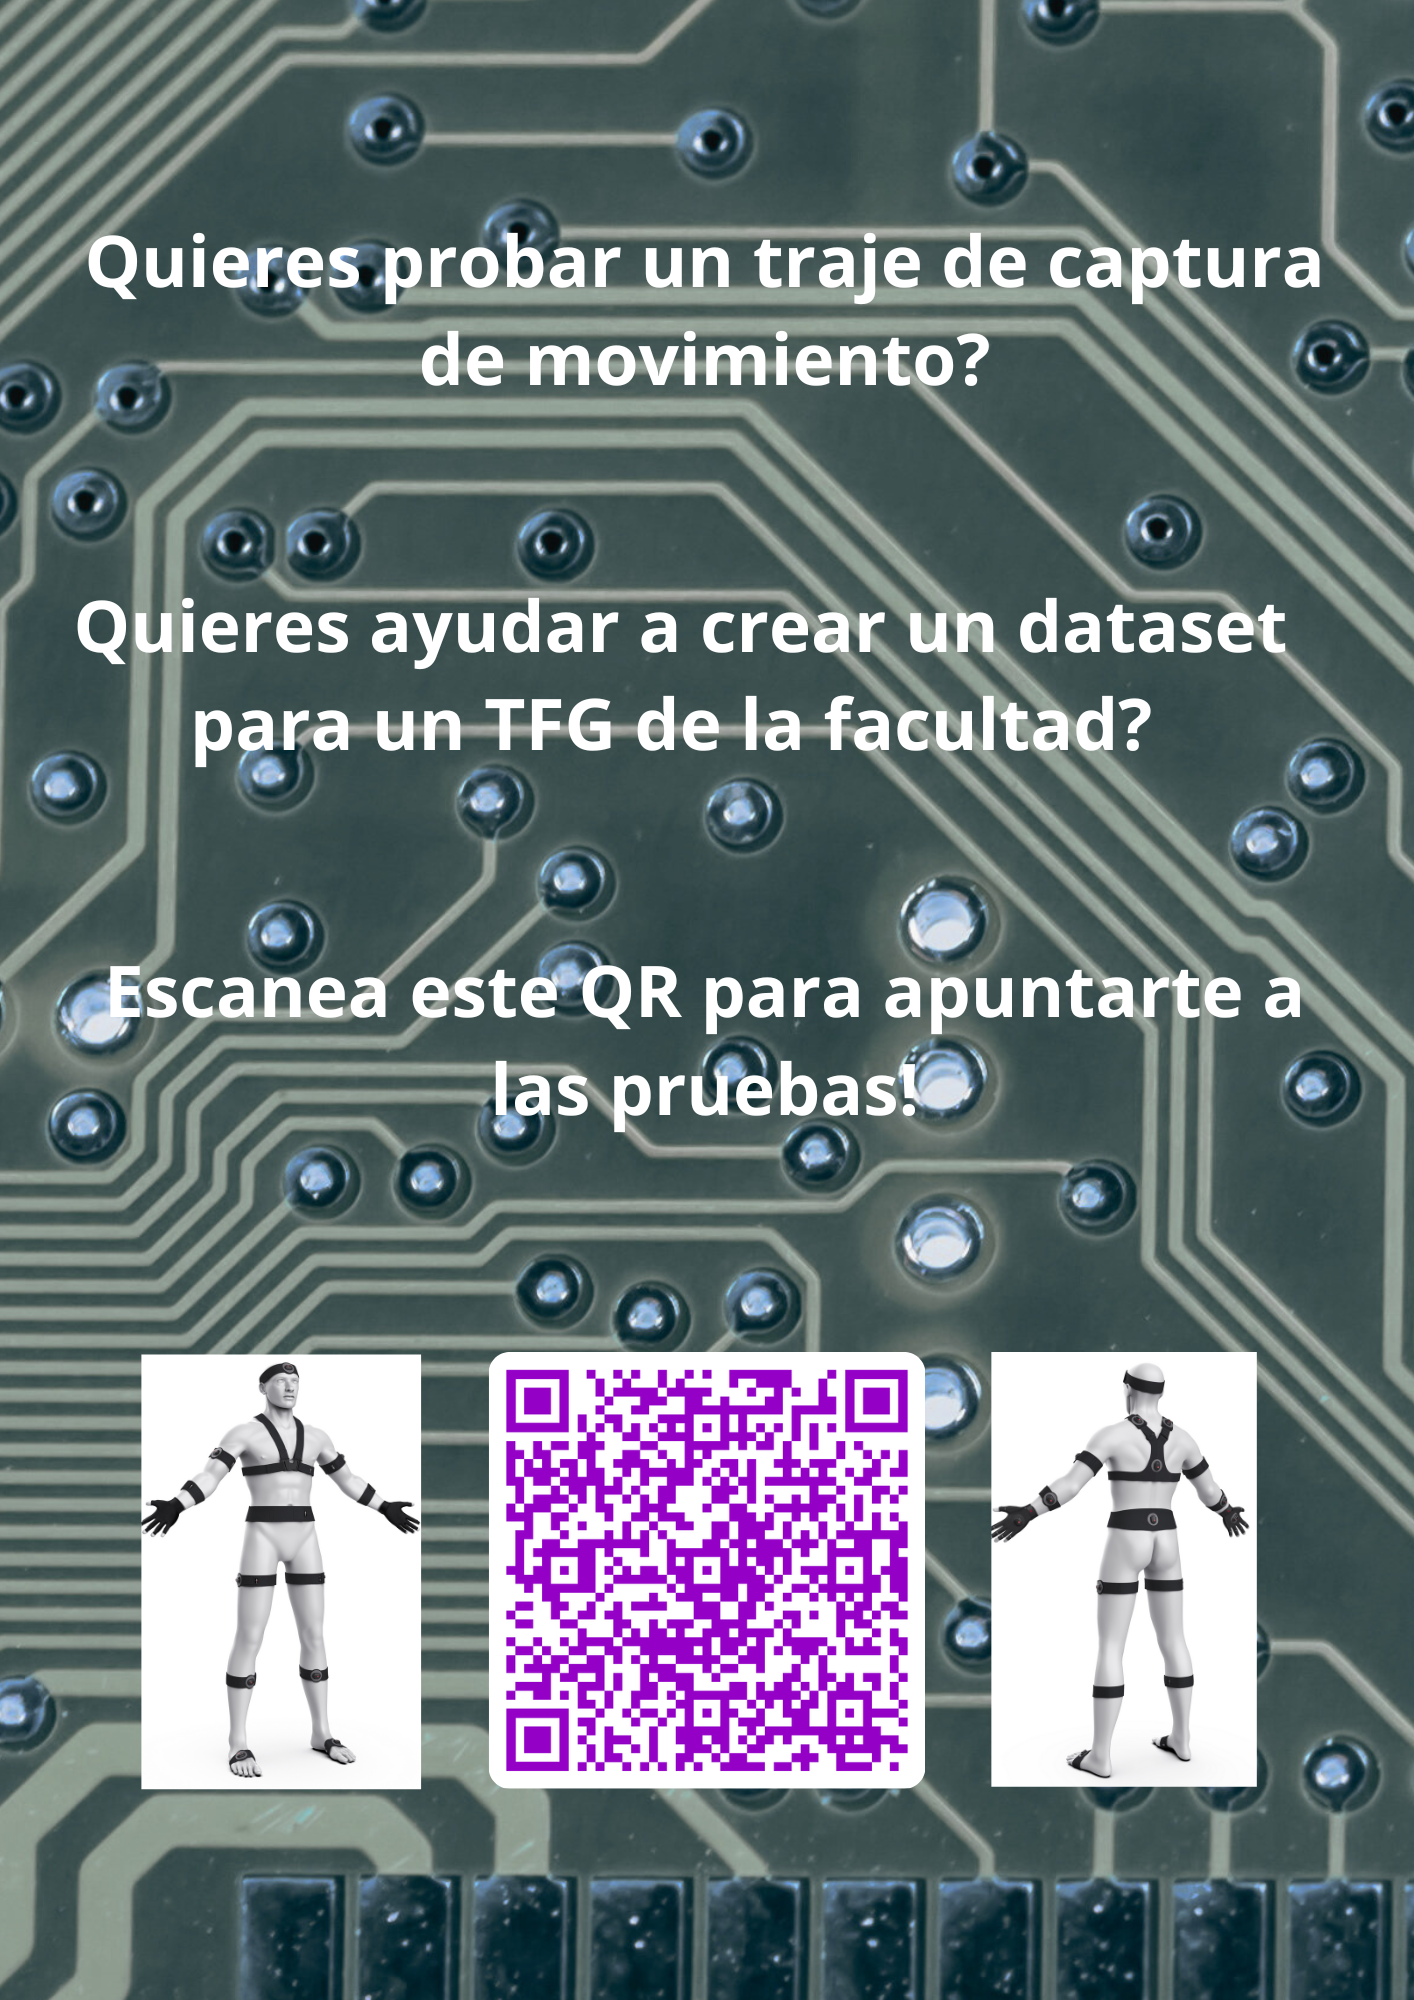
\includegraphics[width=0.7\textwidth]{Imagenes/Bitmap/cartel-imprimir.png}
    \caption{Cartel colgado en la facultad de informática}
    \label{fig:cartel-facultad}
\end{figure}
\begin{figure}[H]
    \centering
    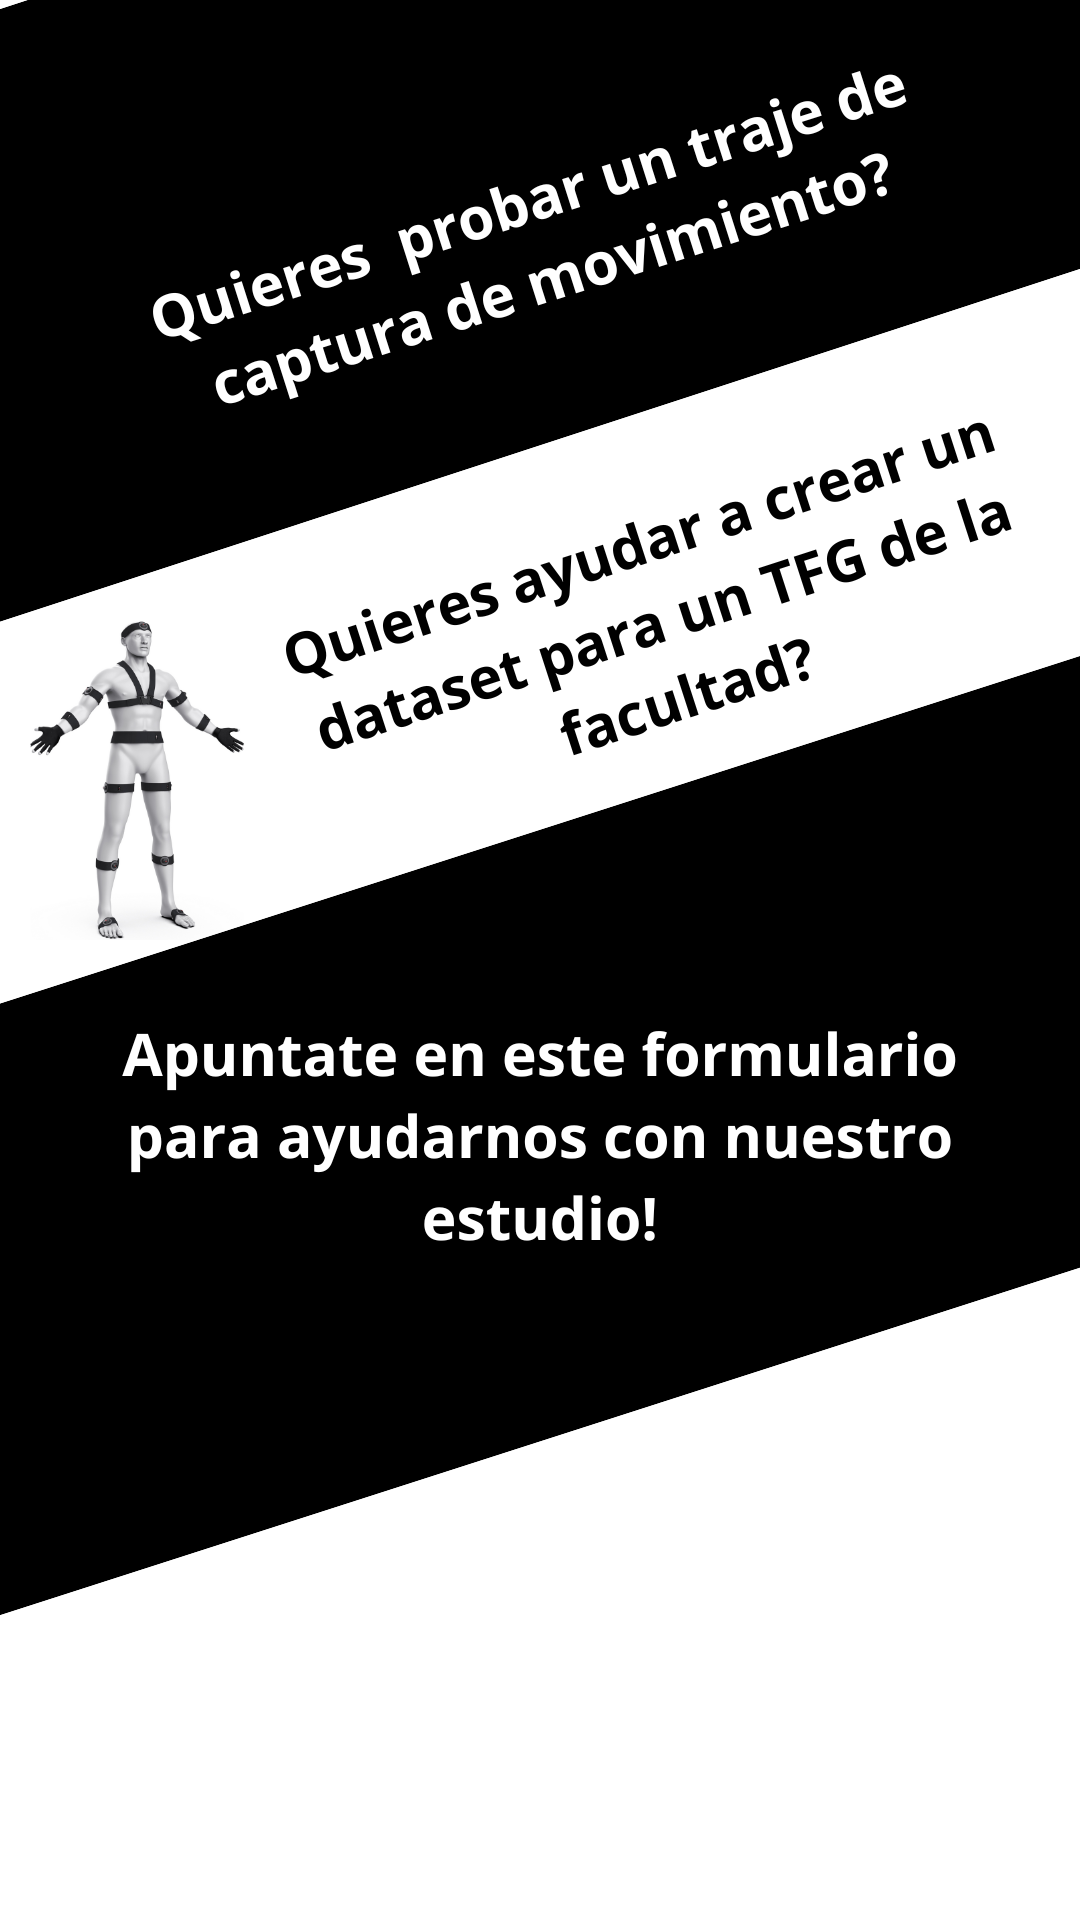
\includegraphics[width=0.7\textwidth]{Imagenes/Bitmap/cartel-instagram.png}
    \caption{Cartel colgado en redes sociales}
    \label{fig:cartel-redes}
\end{figure}

\begin{figure}[H]
    \centering
    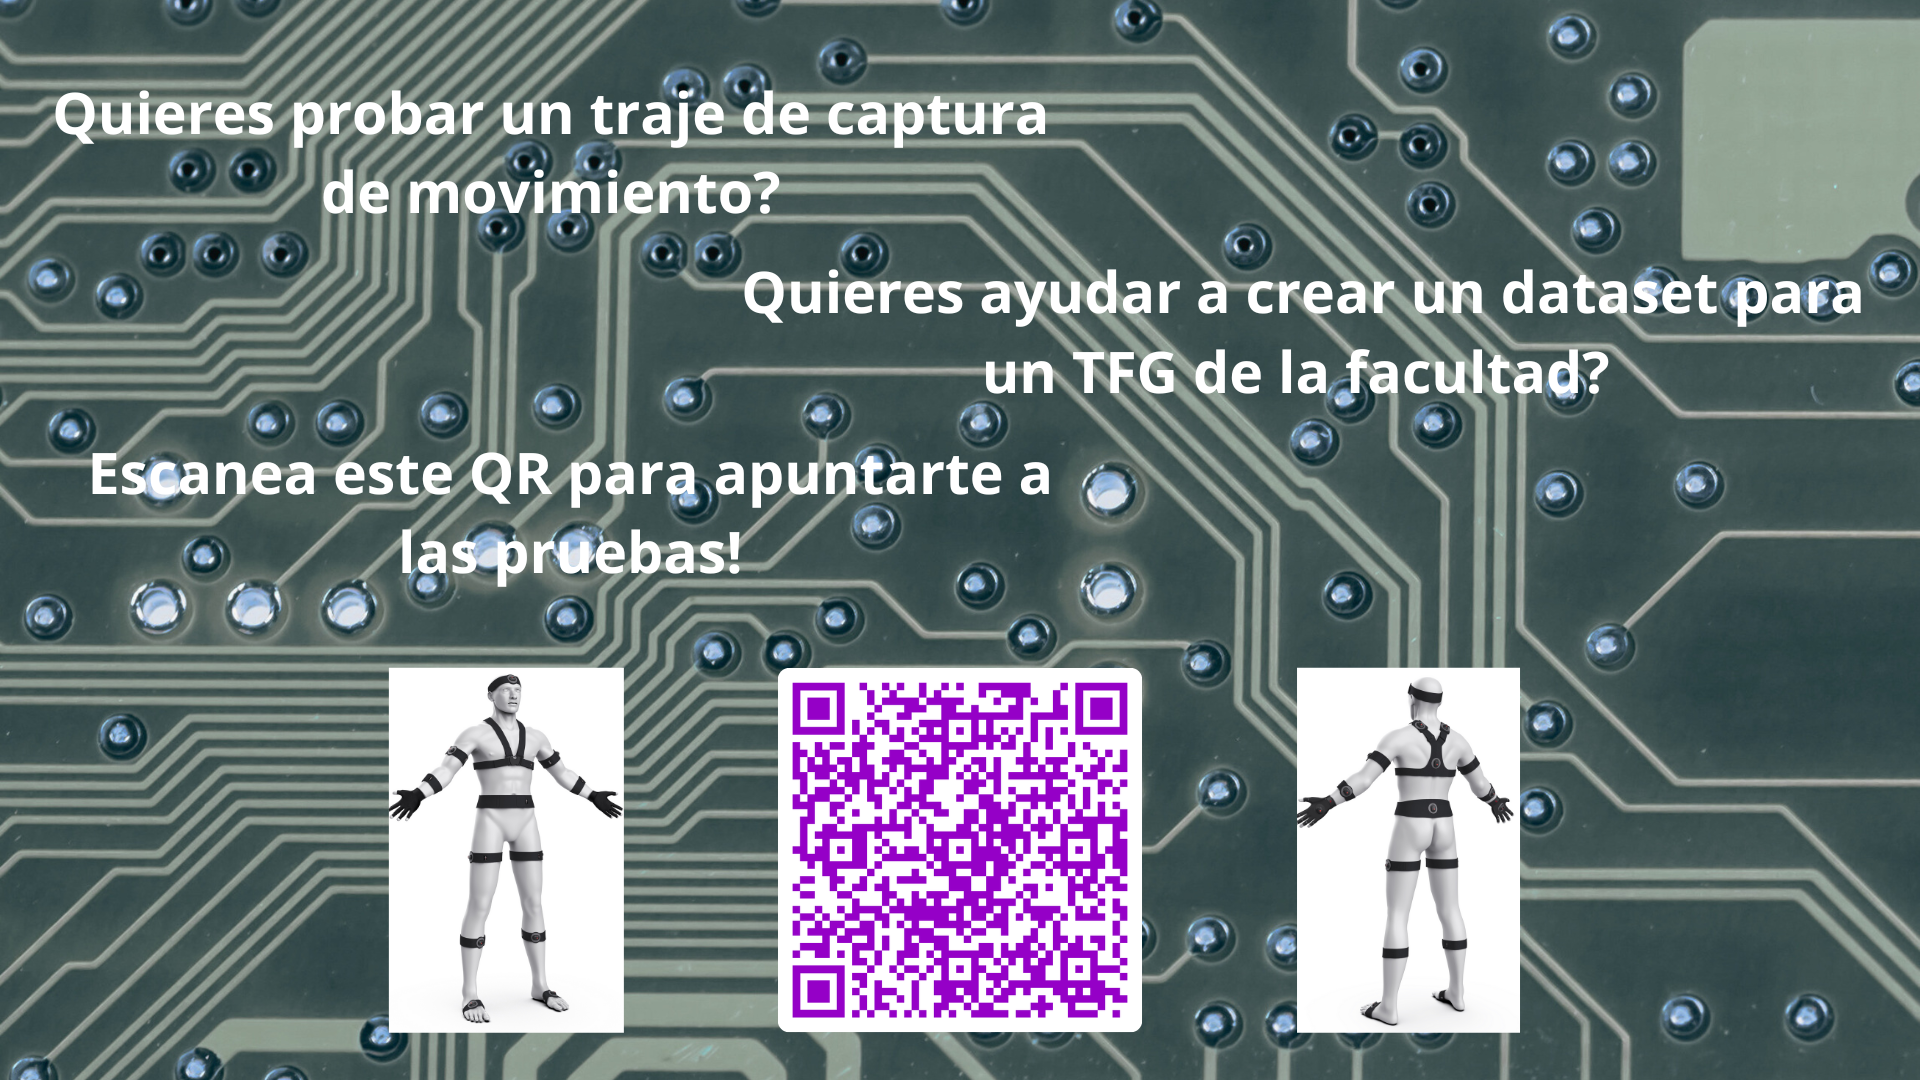
\includegraphics[width=0.7\textwidth]{Imagenes/Bitmap/cartel-pantallas.png}
    \caption{Cartel colgado en pantallas de la facultad}
    \label{fig:cartel-pantallas}
\end{figure}
\chapter{Formulario de recogida de citas}
\label{appendix:formularioCitas}

\begin{figure}[H]
    \centering
    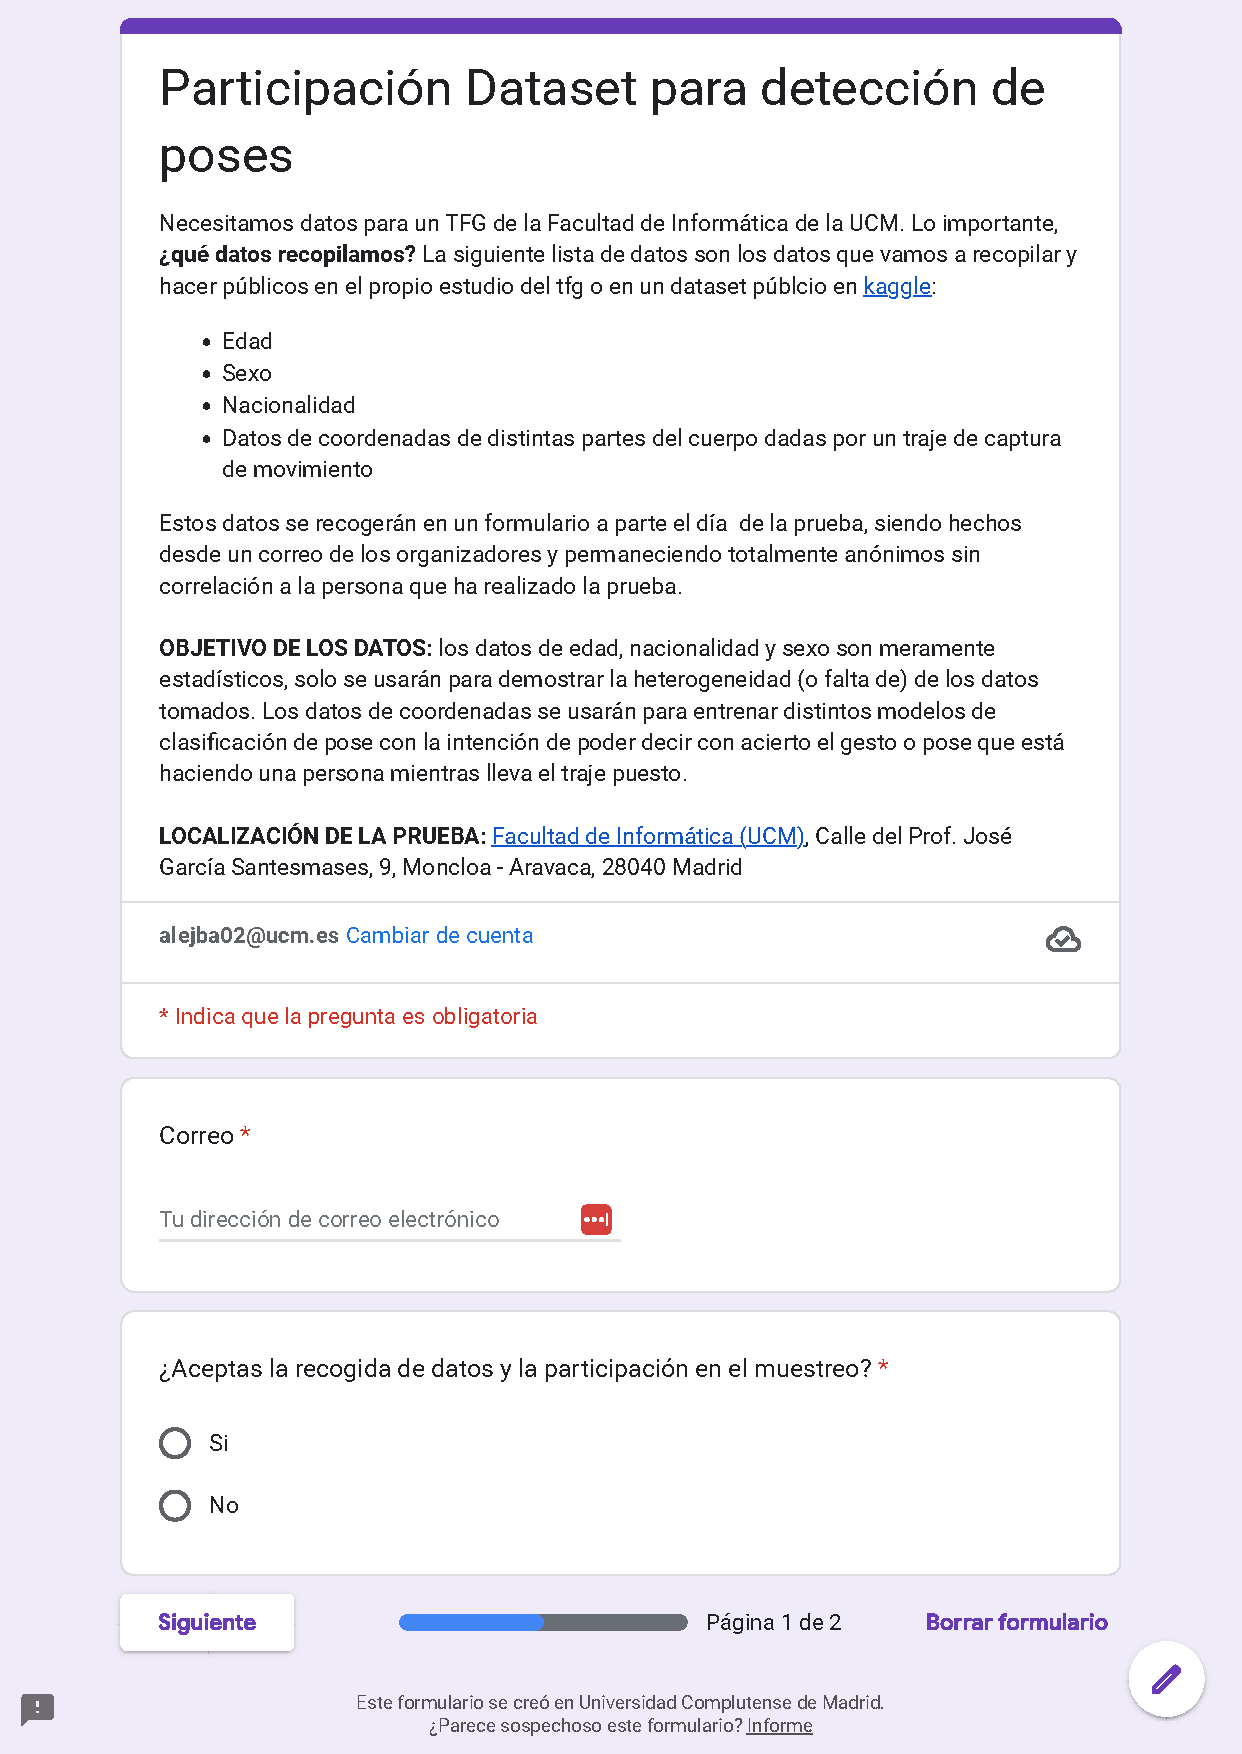
\includegraphics[width=0.7\textwidth]{Imagenes/Vectorial/Form_Participacion1.pdf}
    \caption{Formulario de recogida de citas (primera parte)}
    \label{fig:formulario-citas}
\end{figure}

\begin{figure}[H]
    \centering
    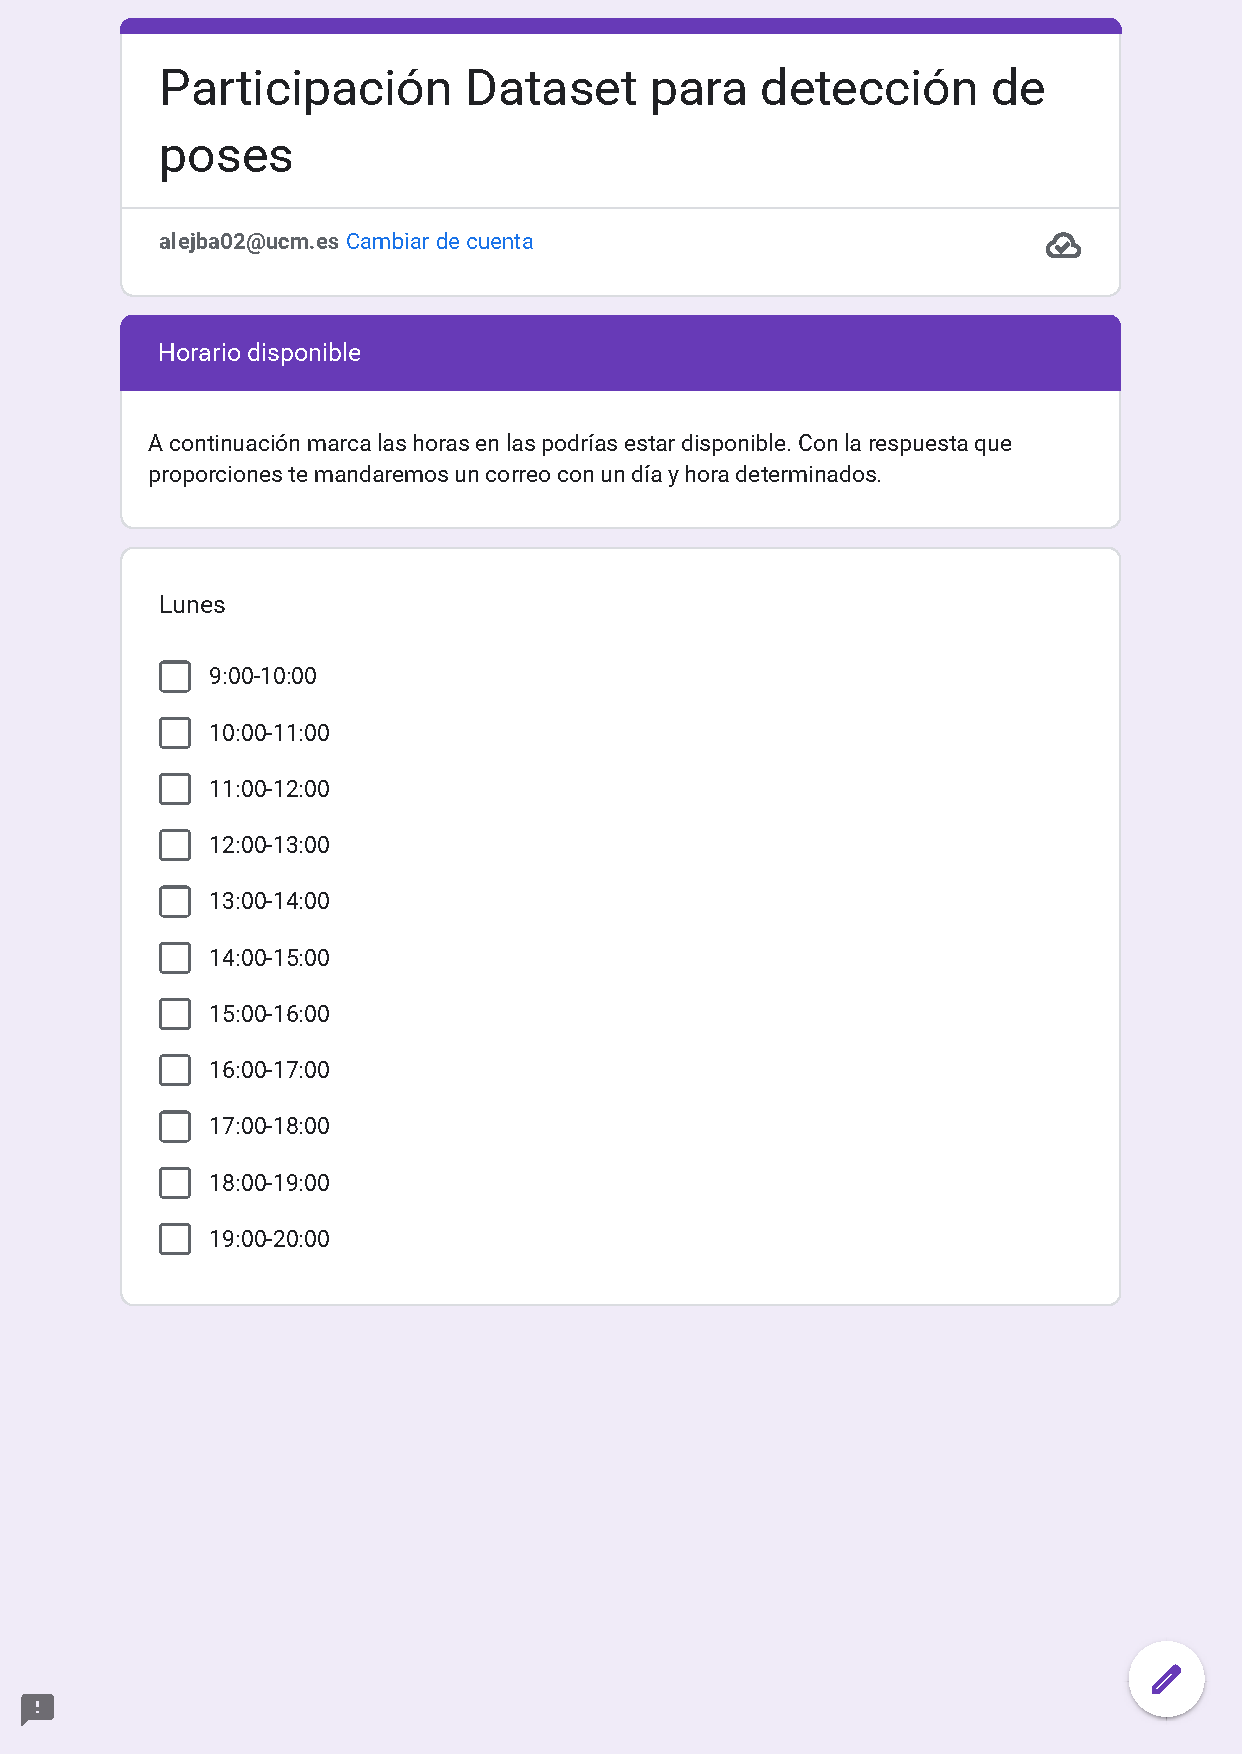
\includegraphics[width=0.7\textwidth]{Imagenes/Vectorial/Form_Participacion2.pdf}
    \caption{Formulario de recogida de citas (segunda parte)}
    \label{fig:formulario-citas-2}
\end{figure}
\chapter{Formulario de recogida de datos demográficos}
\label{appendix:formularioDemografia}

\begin{figure}[H]
    \centering
    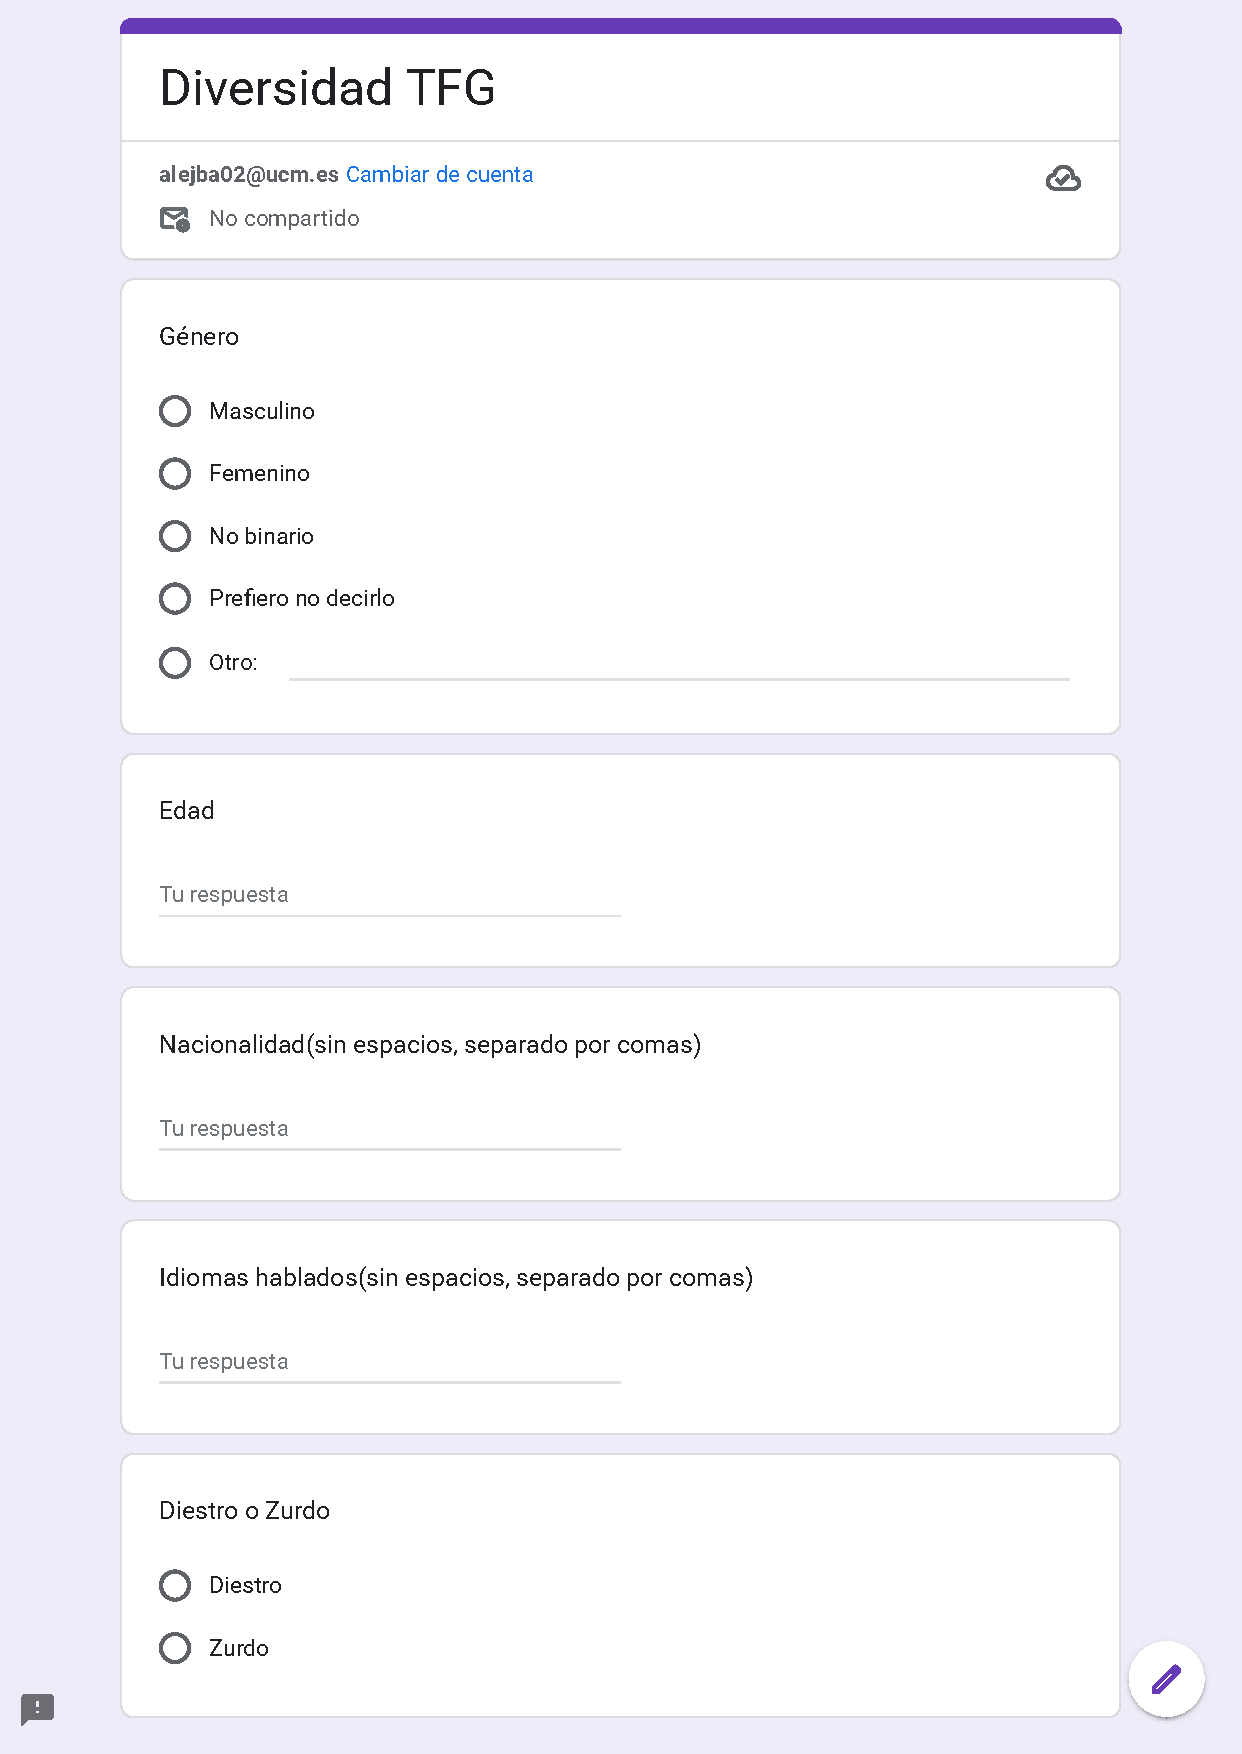
\includegraphics[page=1, width=0.6\textwidth]{Imagenes/Vectorial/Form_Demografia.pdf}
    \caption{Formulario de recogida de datos demográficos (primera parte)}
    \label{fig:formulario-demografia}
\end{figure}

\begin{figure}[H]
    \centering
    \includegraphics[page=2, width=0.6\textwidth]{Imagenes/Vectorial/Form_Demografia.pdf}
    \caption{Formulario de recogida de datos demográficos (segunda parte)}
    \label{fig:formulario-demografia-2}
\end{figure}
\chapter{Gráficos de la generación del dataset}
\label{Appendix:GraficosGenDataset}

\begin{figure}[H]
    \centering
    \includegraphics[width=0.7\textwidth]{Imagenes/Bitmap/Distribución_de_genero_en_las_pruebas.png}
    \caption{Distribución de género de los encuestados}
    \label{fig:muestreo-genero}
\end{figure}

\begin{figure}[H]
    \centering
    \includegraphics[width=0.7\textwidth]{Imagenes/Bitmap/Distribución_de_edad_en_las_pruebas.png}
    \caption{Distribución de edad de los encuestados}
    \label{fig:muestreo-edad}
\end{figure}


\begin{figure}[H]
    \centering
    \includegraphics[width=0.7\textwidth]{Imagenes/Bitmap/Distribución_de_nacionalidades_en_las_pruebas.png}
    \caption{Distribución de nacionalidad de los encuestados}
    \label{fig:muestreo-nacionalidad}
\end{figure}

\begin{figure}[H]
    \centering
    \includegraphics[width=0.7\textwidth]{Imagenes/Bitmap/Distribución_de_idiomas_en_las_pruebas.png}
    \caption{Distribución de idiomas hablados de los encuestados}
    \label{fig:muestreo-idiomas}
\end{figure}

\begin{figure}[H]
    \centering
    \includegraphics[width=0.7\textwidth]{Imagenes/Bitmap/Distribución_de_mano_dominante_en_las_pruebas.png}
    \caption{Distribución de mano dominante de los encuestados}
    \label{fig:muestreo-mano}
\end{figure}
\chapter{Resultados de los distintos modelos \gls{lstm}}
\label{appendix:resultadosLSTM}

La línea verde en los gráficos de tensorboard indican la mejor combinación de hiperparámetos encontrada en cada caso

\section{Intervalo 0.2s}

\begin{figure}[H]
    \centering
    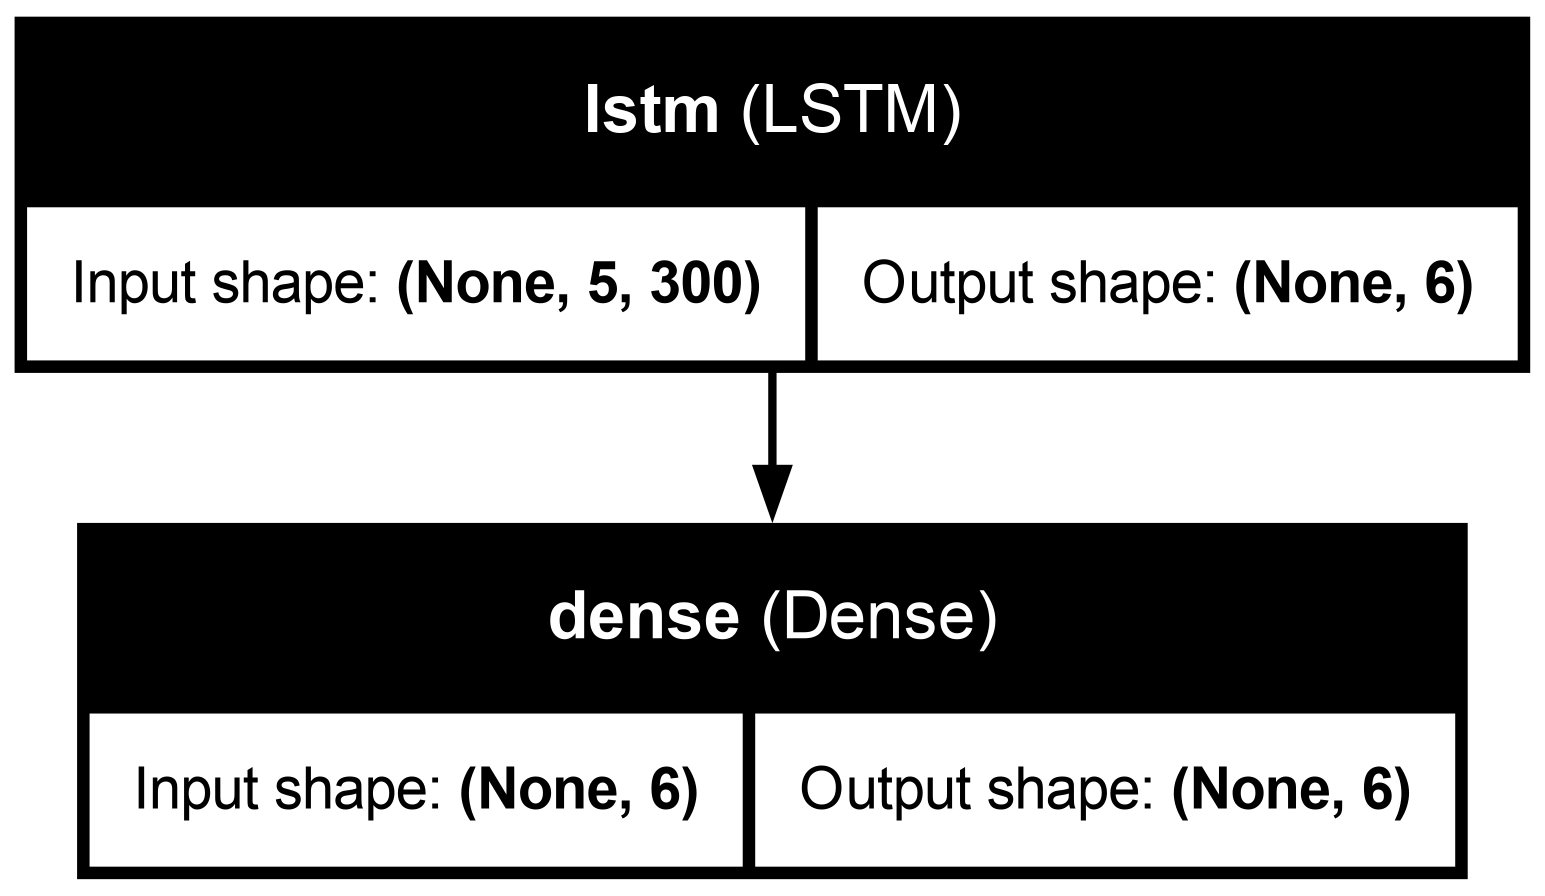
\includegraphics[width=0.3\textwidth]{Imagenes/Bitmap/best-lstm0.2.png}
    \caption{Esquema del modelo LSTM con 0.2s de intervalo}
    \label{fig:lstm-0.2-final}
\end{figure}
\begin{figure}[H]
    \centering
    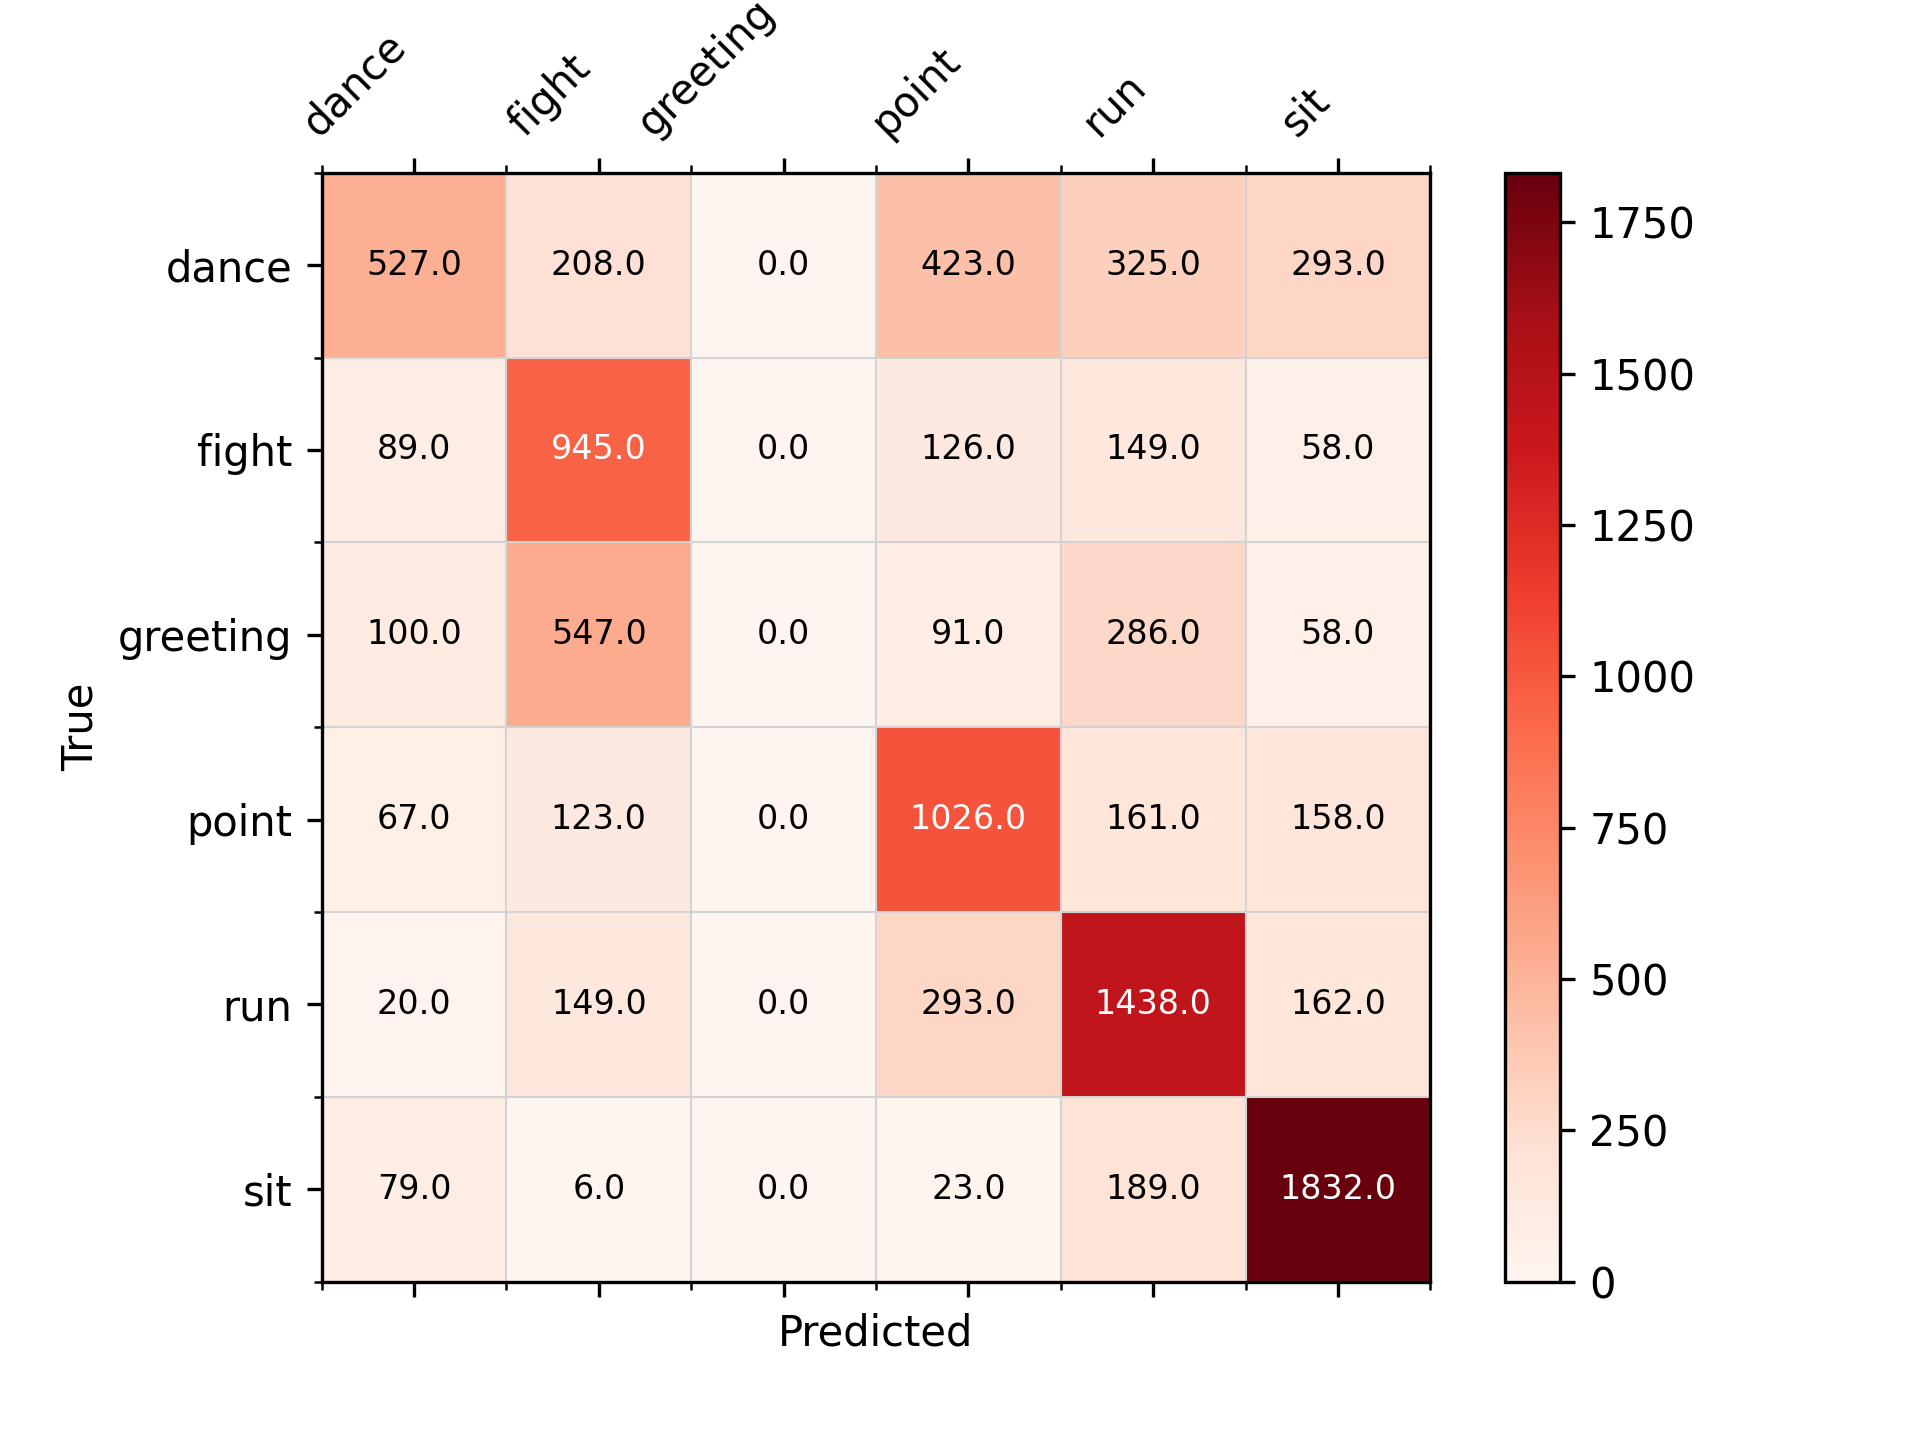
\includegraphics[width=0.6\textwidth]{Imagenes/Bitmap/CM_best-lstm0.2.png}
    \caption{Matriz de confusión del modelo LSTM con 0.2s de intervalo}
    \label{fig:lstm-0.2-matriz}
\end{figure}
\begin{figure}[H]
    \centering
    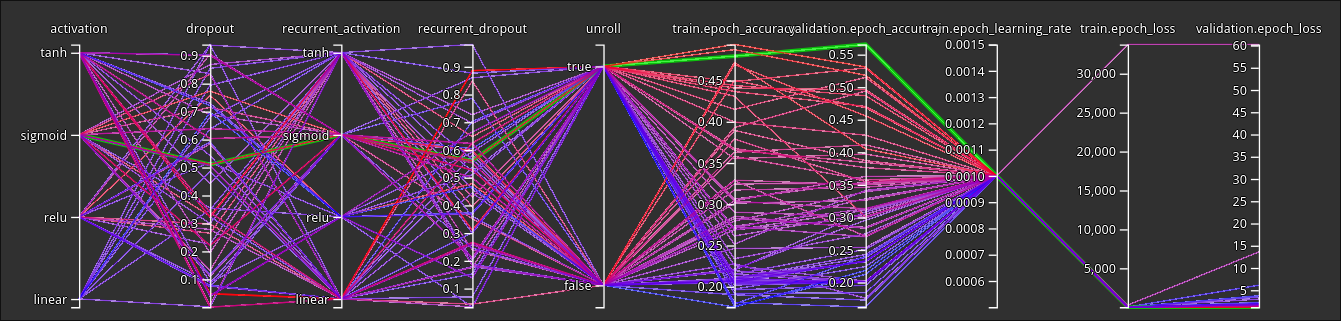
\includegraphics[width=0.8\textwidth]{Imagenes/Bitmap/tb-lstm-0.2.png}
    \caption{Gráfico de entrenamiento del modelo LSTM con 0.2s de intervalo (mejor val\_accuracy = 0.5655)}
    \label{fig:lstm-0.2-grafico}
\end{figure}

\section{Intervalo 0.4s}

\begin{figure}[H]
    \centering
    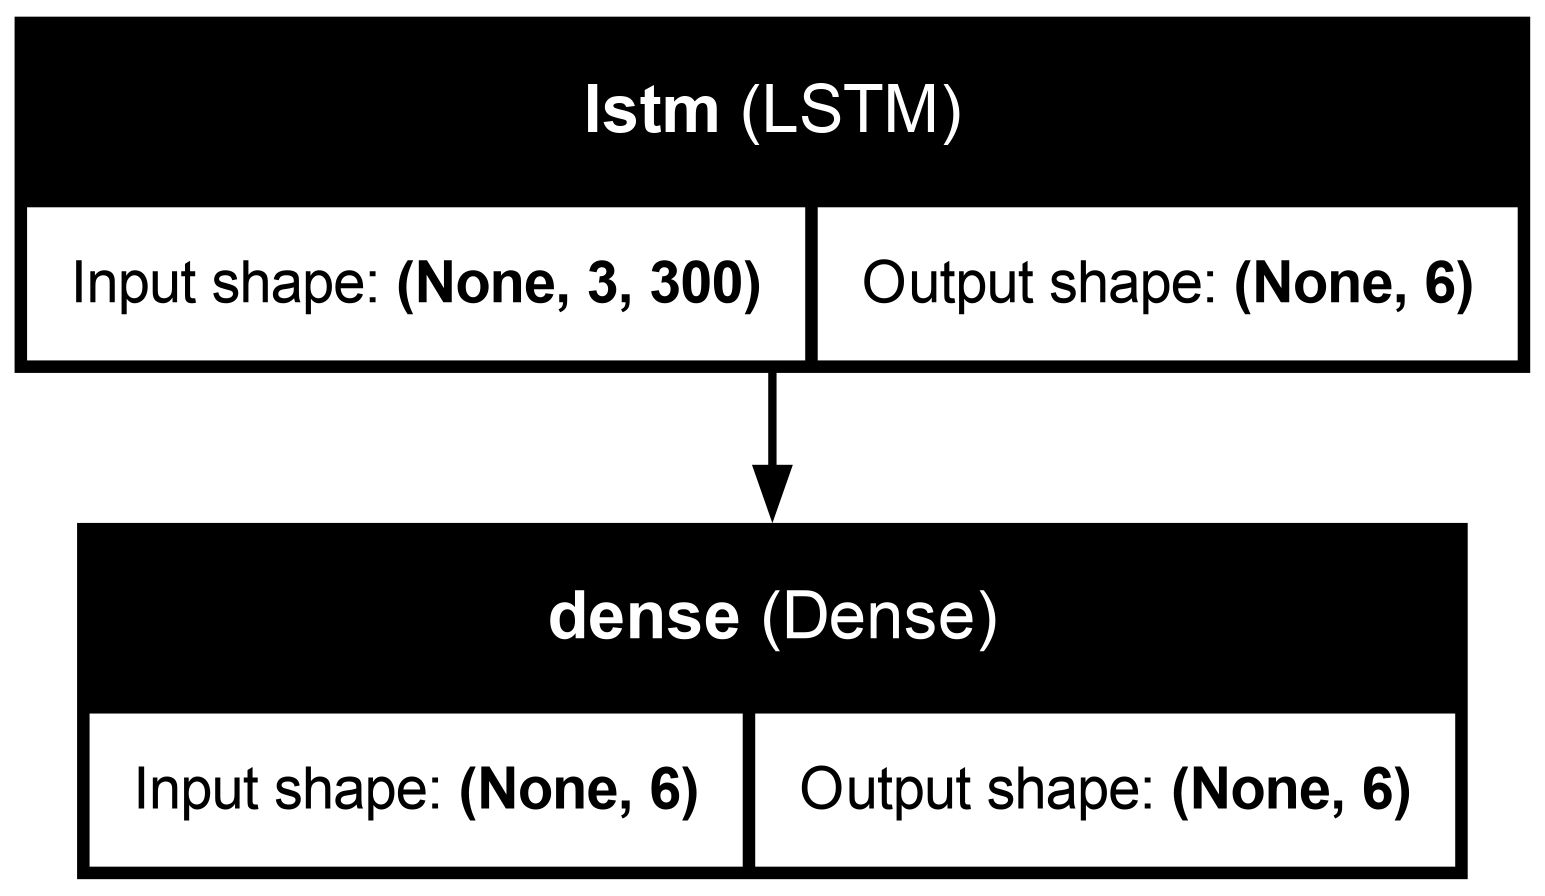
\includegraphics[width=0.3\textwidth]{Imagenes/Bitmap/best-lstm0.4.png}
    \caption{Esquema del modelo LSTM con 0.4s de intervalo}
    \label{fig:lstm-0.4-final}
\end{figure}
\begin{figure}[H]
    \centering
    \includegraphics[width=0.6\textwidth]{Imagenes/Bitmap/CM_best-lstm0.4.png}
    \caption{Matriz de confusión del modelo LSTM con 0.4s de intervalo}
    \label{fig:lstm-0.4-matriz}
\end{figure}

\begin{figure}[H]
    \centering
    \includegraphics[width=0.8\textwidth]{Imagenes/Bitmap/tb-lstm-0.4.png}
    \caption{Gráfico de entrenamiento del modelo LSTM con 0.4s de intervalo (mejor val\_accuracy = 0.5462)}
    \label{fig:lstm-0.4-grafico}
\end{figure}

\section{Intervalo 0.6s}

\begin{figure}[H]
    \centering
    \includegraphics[width=0.3\textwidth]{Imagenes/Bitmap/best-lstm0.6.png}
    \caption{Esquema del modelo LSTM con 0.6s de intervalo}
    \label{fig:lstm-0.6-final}
\end{figure}

\begin{figure}[H]
    \centering
    \includegraphics[width=0.6\textwidth]{Imagenes/Bitmap/CM_best-lstm0.6.png}
    \caption{Matriz de confusión del modelo LSTM con 0.6s de intervalo}
    \label{fig:lstm-0.6-matriz}
\end{figure}

\begin{figure}[H]
    \centering
    \includegraphics[width=0.8\textwidth]{Imagenes/Bitmap/tb-lstm-0.6.png}
    \caption{Gráfico de entrenamiento del modelo LSTM con 0.6s de intervalo (mejor val\_accuracy = 0.5301)}
    \label{fig:lstm-0.6-grafico}
\end{figure}

\section{Intervalo 0.8s}

\begin{figure}[H]
    \centering
    \includegraphics[width=0.3\textwidth]{Imagenes/Bitmap/best-lstm0.8.png}
    \caption{Esquema del modelo LSTM con 0.8s de intervalo}
    \label{fig:lstm-0.8-final}
\end{figure}

\begin{figure}[H]
    \centering
    \includegraphics[width=0.6\textwidth]{Imagenes/Bitmap/CM_best-lstm0.8.png}
    \caption{Matriz de confusión del modelo LSTM con 0.8s de intervalo}
    \label{fig:lstm-0.8-matriz}
\end{figure}

\begin{figure}[H]
    \centering
    \includegraphics[width=0.8\textwidth]{Imagenes/Bitmap/tb-lstm-0.8.png}
    \caption{Gráfico de entrenamiento del modelo LSTM con 0.8s de intervalo (mejor val\_accuracy = 0.5912)}
    \label{fig:lstm-0.8-grafico}
\end{figure}

\section{Intervalo 1.0s}

\begin{figure}[H]
    \centering
    \includegraphics[width=0.3\textwidth]{Imagenes/Bitmap/best-lstm1.png}
    \caption{Esquema del modelo LSTM con 1.0s de intervalo}
    \label{fig:lstm-1.0-final}
\end{figure}

\begin{figure}[H]
    \centering
    \includegraphics[width=0.6\textwidth]{Imagenes/Bitmap/CM_best-lstm1.png}
    \caption{Matriz de confusión del modelo LSTM con 1.0s de intervalo}
    \label{fig:lstm-1.0-matriz}
\end{figure}

\begin{figure}[H]
    \centering
    \includegraphics[width=0.8\textwidth]{Imagenes/Bitmap/tb-lstm-1.0.png}
    \caption{Gráfico de entrenamiento del modelo LSTM con 1.0s de intervalo (mejor val\_accuracy = 0.5318)}
    \label{fig:lstm-1.0-grafico}
\end{figure}
\chapter{Resultados de los distintos modelos \gls{rnn}}
\label{appendix:resultadosRNN}

La línea verde en los gráficos de tensorboard indican la mejor combinación de hiperparámetos encontrada en cada caso

\section{Intervalo 0.2s}

\begin{figure}[H]
    \centering
    \includegraphics[width=0.3\textwidth]{Imagenes/Bitmap/best-rnn0.2.png}
    \caption{Esquema del modelo RNN con 0.2s de intervalo}
    \label{fig:rnn-0.2-final}
\end{figure}
\begin{figure}[H]
    \centering
    \includegraphics[width=0.6\textwidth]{Imagenes/Bitmap/CM_best-rnn0.2.png}
    \caption{Matriz de confusión del modelo RNN con 0.2s de intervalo}
    \label{fig:rnn-0.2-matriz}
\end{figure}
\begin{figure}[H]
    \centering
    \includegraphics[width=0.8\textwidth]{Imagenes/Bitmap/tb-rnn-0.2.png}
    \caption{Gráfico de entrenamiento del modelo RNN con 0.2s de intervalo (mejor val\_accuracy = 0.3486)}
    \label{fig:rnn-0.2-grafico}
\end{figure}

\section{Intervalo 0.4s}

\begin{figure}[H]
    \centering
    \includegraphics[width=0.3\textwidth]{Imagenes/Bitmap/best-rnn0.4.png}
    \caption{Esquema del modelo RNN con 0.4s de intervalo}
    \label{fig:rnn-0.4-final}
\end{figure}
\begin{figure}[H]
    \centering
    \includegraphics[width=0.6\textwidth]{Imagenes/Bitmap/CM_best-rnn0.4.png}
    \caption{Matriz de confusión del modelo RNN con 0.4s de intervalo}
    \label{fig:rnn-0.4-matriz}
\end{figure}

\begin{figure}[H]
    \centering
    \includegraphics[width=0.8\textwidth]{Imagenes/Bitmap/tb-rnn-0.4.png}
    \caption{Gráfico de entrenamiento del modelo RNN con 0.4s de intervalo (mejor val\_accuracy = 0.4535)}
    \label{fig:rnn-0.4-grafico}
\end{figure}

\section{Intervalo 0.6s}

\begin{figure}[H]
    \centering
    \includegraphics[width=0.3\textwidth]{Imagenes/Bitmap/best-rnn0.6.png}
    \caption{Esquema del modelo RNN con 0.6s de intervalo}
    \label{fig:rnn-0.6-final}
\end{figure}

\begin{figure}[H]
    \centering
    \includegraphics[width=0.6\textwidth]{Imagenes/Bitmap/CM_best-rnn0.6.png}
    \caption{Matriz de confusión del modelo RNN con 0.6s de intervalo}
    \label{fig:rnn-0.6-matriz}
\end{figure}

\begin{figure}[H]
    \centering
    \includegraphics[width=0.8\textwidth]{Imagenes/Bitmap/tb-rnn-0.6.png}
    \caption{Gráfico de entrenamiento del modelo RNN con 0.6s de intervalo (mejor val\_accuracy = 0.41185)}
    \label{fig:rnn-0.6-grafico}
\end{figure}

\section{Intervalo 0.8s}

\begin{figure}[H]
    \centering
    \includegraphics[width=0.3\textwidth]{Imagenes/Bitmap/best-rnn0.8.png}
    \caption{Esquema del modelo RNN con 0.8s de intervalo}
    \label{fig:rnn-0.8-final}
\end{figure}

\begin{figure}[H]
    \centering
    \includegraphics[width=0.6\textwidth]{Imagenes/Bitmap/CM_best-rnn0.8.png}
    \caption{Matriz de confusión del modelo RNN con 0.8s de intervalo}
    \label{fig:rnn-0.8-matriz}
\end{figure}

\begin{figure}[H]
    \centering
    \includegraphics[width=0.8\textwidth]{Imagenes/Bitmap/tb-rnn-0.8.png}
    \caption{Gráfico de entrenamiento del modelo RNN con 0.8s de intervalo (mejor val\_accuracy = 0.47865)}
    \label{fig:rnn-0.8-grafico}
\end{figure}

\section{Intervalo 1.0s}

\begin{figure}[H]
    \centering
    \includegraphics[width=0.3\textwidth]{Imagenes/Bitmap/best-rnn1.0.png}
    \caption{Esquema del modelo RNN con 1.0s de intervalo}
    \label{fig:rnn-1.0-final}
\end{figure}

\begin{figure}[H]
    \centering
    \includegraphics[width=0.6\textwidth]{Imagenes/Bitmap/CM_best-rnn1.0.png}
    \caption{Matriz de confusión del modelo RNN con 1.0s de intervalo}
    \label{fig:rnn-1.0-matriz}
\end{figure}

\begin{figure}[H]
    \centering
    \includegraphics[width=0.8\textwidth]{Imagenes/Bitmap/tb-rnn-1.0.png}
    \caption{Gráfico de entrenamiento del modelo RNN con 1.0s de intervalo (mejor val\_accuracy = 0.39377)}
    \label{fig:rnn-1.0-grafico}
\end{figure}
\chapter{Resultados de los distintos modelos \gls{cnn}}
\label{appendix:resultadosCNN}

La línea verde en los gráficos de tensorboard indican la mejor combinación de hiperparámetos encontrada en cada caso

\section{Intervalo 0.2s}

\begin{figure}[H]
    \centering
    \includegraphics[width=0.3\textwidth]{Imagenes/Bitmap/best-cnn0.2.png}
    \caption{Esquema del modelo CNN con 0.2s de intervalo}
    \label{fig:cnn-0.2-final}
\end{figure}
\begin{figure}[H]
    \centering
    \includegraphics[width=0.6\textwidth]{Imagenes/Bitmap/CM_best-cnn0.2.png}
    \caption{Matriz de confusión del modelo CNN con 0.2s de intervalo}
    \label{fig:cnn-0.2-matriz}
\end{figure}
\begin{figure}[H]
    \centering
    \includegraphics[width=0.8\textwidth]{Imagenes/Bitmap/tb-cnn-0.2.png}
    \caption{Gráfico de entrenamiento del modelo CNN con 0.2s de intervalo (mejor val\_accuracy = 0.28777)}
    \label{fig:cnn-0.2-grafico}
\end{figure}

\section{Intervalo 0.4s}

\begin{figure}[H]
    \centering
    \includegraphics[width=0.3\textwidth]{Imagenes/Bitmap/best-cnn0.4.png}
    \caption{Esquema del modelo CNN con 0.4s de intervalo}
    \label{fig:cnn-0.4-final}
\end{figure}
\begin{figure}[H]
    \centering
    \includegraphics[width=0.6\textwidth]{Imagenes/Bitmap/CM_best-cnn0.4.png}
    \caption{Matriz de confusión del modelo CNN con 0.4s de intervalo}
    \label{fig:cnn-0.4-matriz}
\end{figure}

\begin{figure}[H]
    \centering
    \includegraphics[width=0.8\textwidth]{Imagenes/Bitmap/tb-cnn-0.4.png}
    \caption{Gráfico de entrenamiento del modelo CNN con 0.4s de intervalo (mejor val\_accuracy = 0.49473)}
    \label{fig:cnn-0.4-grafico}
\end{figure}

\section{Intervalo 0.6s}

\begin{figure}[H]
    \centering
    \includegraphics[width=0.3\textwidth]{Imagenes/Bitmap/best-cnn0.6.png}
    \caption{Esquema del modelo CNN con 0.6s de intervalo}
    \label{fig:cnn-0.6-final}
\end{figure}

\begin{figure}[H]
    \centering
    \includegraphics[width=0.6\textwidth]{Imagenes/Bitmap/CM_best-cnn0.6.png}
    \caption{Matriz de confusión del modelo CNN con 0.6s de intervalo}
    \label{fig:cnn-0.6-matriz}
\end{figure}

\begin{figure}[H]
    \centering
    \includegraphics[width=0.8\textwidth]{Imagenes/Bitmap/tb-cnn-0.6.png}
    \caption{Gráfico de entrenamiento del modelo CNN con 0.6s de intervalo (mejor val\_accuracy = 0.44952)}
    \label{fig:cnn-0.6-grafico}
\end{figure}

\section{Intervalo 0.8s}

\begin{figure}[H]
    \centering
    \includegraphics[width=0.3\textwidth]{Imagenes/Bitmap/best-cnn0.8.png}
    \caption{Esquema del modelo CNN con 0.8s de intervalo}
    \label{fig:cnn-0.8-final}
\end{figure}

\begin{figure}[H]
    \centering
    \includegraphics[width=0.6\textwidth]{Imagenes/Bitmap/CM_best-cnn0.8.png}
    \caption{Matriz de confusión del modelo CNN con 0.8s de intervalo}
    \label{fig:cnn-0.8-matriz}
\end{figure}

\begin{figure}[H]
    \centering
    \includegraphics[width=0.8\textwidth]{Imagenes/Bitmap/tb-cnn-0.8.png}
    \caption{Gráfico de entrenamiento del modelo CNN con 0.8s de intervalo (mejor val\_accuracy = 0.40583)}
    \label{fig:cnn-0.8-grafico}
\end{figure}

\section{Intervalo 1.0s}

\begin{figure}[H]
    \centering
    \includegraphics[width=0.3\textwidth]{Imagenes/Bitmap/best-cnn1.0.png}
    \caption{Esquema del modelo CNN con 1.0s de intervalo}
    \label{fig:cnn-1.0-final}
\end{figure}

\begin{figure}[H]
    \centering
    \includegraphics[width=0.6\textwidth]{Imagenes/Bitmap/CM_best-cnn1.0.png}
    \caption{Matriz de confusión del modelo CNN con 1.0s de intervalo}
    \label{fig:cnn-1.0-matriz}
\end{figure}

\begin{figure}[H]
    \centering
    \includegraphics[width=0.8\textwidth]{Imagenes/Bitmap/tb-cnn-1.0.png}
    \caption{Gráfico de entrenamiento del modelo CNN con 1.0s de intervalo (mejor val\_accuracy = 0.56002)}
    \label{fig:cnn-1.0-grafico}
\end{figure}
\chapter{Resultados de los distintos modelos \gls{randomforest}}
\label{appendix:resultadosRF}

\section{Intervalo 0.2s}

\begin{figure}[H]
    \centering
    \includegraphics[width=0.6\textwidth]{Imagenes/Bitmap/CM_best_rf_0.2.png}
    \caption{Matriz de confusión del modelo Random Forest con 0.2s de intervalo (mejor val\_accuracy = 0.85735)}
    \label{fig:rf-0.2-matriz}
\end{figure}

\section{Intervalo 0.4s}

\begin{figure}[H]
    \centering
    \includegraphics[width=0.6\textwidth]{Imagenes/Bitmap/CM_best_rf_0.4.png}
    \caption{Matriz de confusión del modelo Random Forest con 0.4s de intervalo (mejor val\_accuracy = 0.85735)}
    \label{fig:rf-0.4-matriz}
\end{figure}

\section{Intervalo 0.6s}

\begin{figure}[H]
    \centering
    \includegraphics[width=0.6\textwidth]{Imagenes/Bitmap/CM_best_rf_0.6.png}
    \caption{Matriz de confusión del modelo Random Forest con 0.6s de intervalo (mejor val\_accuracy = 0.85233)}
    \label{fig:rf-0.6-matriz}
\end{figure}

\section{Intervalo 0.8s}

\begin{figure}[H]
    \centering
    \includegraphics[width=0.6\textwidth]{Imagenes/Bitmap/CM_best_rf_0.8.png}
    \caption{Matriz de confusión del modelo Random Forest con 0.8s de intervalo (mejor val\_accuracy = 0.85936)}
    \label{fig:rf-0.8-matriz}
\end{figure}

\section{Intervalo 1.0s}

\begin{figure}[H]
    \centering
    \includegraphics[width=0.6\textwidth]{Imagenes/Bitmap/CM_best_rf_1.0.png}
    \caption{Matriz de confusión del modelo Random Forest con 1.0s de intervalo (mejor val\_accuracy = 0.84681)}
    \label{fig:rf-1.0-matriz}
\end{figure}
%\include{...}
%\include{...}
%\include{...}
\backmatter



%
% Índice de palabras
%

% Sólo  la   generamos  si  está   declarada  \generaindice.  Consulta
% TeXiS.sty para más información.

% En realidad, el soporte para la generación de índices de palabras
% en TeXiS no está documentada en el manual, porque no ha sido usada
% "en producción". Por tanto, el fichero que genera el índice
% *no* se incluye aquí (está comentado). Consulta la documentación
% en TeXiS_pream.tex para más información.
\ifx\generaindice\undefined
\else
  %%---------------------------------------------------------------------
%
%                        TeXiS_indice.tex
%
%---------------------------------------------------------------------
%
% TeXiS_indice.tex
% Copyright 2009 Marco Antonio Gomez-Martin, Pedro Pablo Gomez-Martin
%
% This file belongs to TeXiS, a LaTeX template for writting
% Thesis and other documents. The complete last TeXiS package can
% be obtained from http://gaia.fdi.ucm.es/projects/texis/
%
% This work may be distributed and/or modified under the
% conditions of the LaTeX Project Public License, either version 1.3
% of this license or (at your option) any later version.
% The latest version of this license is in
%   http://www.latex-project.org/lppl.txt
% and version 1.3 or later is part of all distributions of LaTeX
% version 2005/12/01 or later.
%
% This work has the LPPL maintenance status `maintained'.
% 
% The Current Maintainers of this work are Marco Antonio Gomez-Martin
% and Pedro Pablo Gomez-Martin
%
%---------------------------------------------------------------------
%
% Contiene  los  comandos  para  generar  el índice  de  palabras  del
% documento.
%
%---------------------------------------------------------------------
%
% NOTA IMPORTANTE: el  soporte en TeXiS para el  índice de palabras es
% embrionario, y  de hecho  ni siquiera se  describe en el  manual. Se
% proporciona  una infraestructura  básica (sin  terminar)  para ello,
% pero  no ha  sido usada  "en producción".  De hecho,  a pesar  de la
% existencia de  este fichero, *no* se incluye  en Tesis.tex. Consulta
% la documentación en TeXiS_pream.tex para más información.
%
%---------------------------------------------------------------------


% Si se  va a generar  la tabla de  contenidos (el índice  habitual) y
% también vamos a  generar el índice de palabras  (ambas decisiones se
% toman en  función de  la definición  o no de  un par  de constantes,
% puedes consultar modo.tex para más información), entonces metemos en
% la tabla de contenidos una  entrada para marcar la página donde está
% el índice de palabras.

\ifx\generatoc\undefined
\else
   \addcontentsline{toc}{chapter}{\indexname}
\fi


% Generamos el índice
\printindex

% Variable local para emacs, para  que encuentre el fichero maestro de
% compilación y funcionen mejor algunas teclas rápidas de AucTeX

%%%
%%% Local Variables:
%%% mode: latex
%%% TeX-master: "./tesis.tex"
%%% End:

\fi

%
% Lista de acrónimos
%

% Sólo  lo  generamos  si  está declarada  \generaacronimos.  Consulta
% TeXiS.sty para más información.


\ifx\generaacronimos\undefined
\else
  %---------------------------------------------------------------------
%
%                        TeXiS_acron.tex
%
%---------------------------------------------------------------------
%
% TeXiS_acron.tex
% Copyright 2009 Marco Antonio Gomez-Martin, Pedro Pablo Gomez-Martin
%
% This file belongs to TeXiS, a LaTeX template for writting
% Thesis and other documents. The complete last TeXiS package can
% be obtained from http://gaia.fdi.ucm.es/projects/texis/
%
% This work may be distributed and/or modified under the
% conditions of the LaTeX Project Public License, either version 1.3
% of this license or (at your option) any later version.
% The latest version of this license is in
%   http://www.latex-project.org/lppl.txt
% and version 1.3 or later is part of all distributions of LaTeX
% version 2005/12/01 or later.
%
% This work has the LPPL maintenance status `maintained'.
% 
% The Current Maintainers of this work are Marco Antonio Gomez-Martin
% and Pedro Pablo Gomez-Martin
%
%---------------------------------------------------------------------
%
% Contiene  los  comandos  para  generar  el listado de acrónimos
% documento.
%
%---------------------------------------------------------------------
%
% NOTA IMPORTANTE:  para que la  generación de acrónimos  funcione, al
% menos  debe  existir  un  acrónimo   en  el  documento.  Si  no,  la
% compilación  del   fichero  LaTeX  falla  con   un  error  "extraño"
% (indicando  que  quizá  falte  un \item).   Consulta  el  comentario
% referente al paquete glosstex en TeXiS_pream.tex.
%
%---------------------------------------------------------------------


% Redefinimos a español  el título de la lista  de acrónimos (Babel no
% lo hace por nosotros esta vez)

\def\listacronymname{Lista de acrónimos}

% Para el glosario:
% \def\glosarryname{Glosario}

% Si se  va a generar  la tabla de  contenidos (el índice  habitual) y
% también vamos a  generar la lista de acrónimos  (ambas decisiones se
% toman en  función de  la definición  o no de  un par  de constantes,
% puedes consultar config.tex  para más información), entonces metemos
% en la  tabla de contenidos una  entrada para marcar  la página donde
% está el índice de palabras.



% Generamos la lista de acrónimos (en realidad el índice asociado a la
% lista "acr" de GlossTeX)
\cleardoublepage
% \addcontentsline{toc}{chapter}{Glosario}
\printglossaries


% Variable local para emacs, para  que encuentre el fichero maestro de
% compilación y funcionen mejor algunas teclas rápidas de AucTeX

%%%
%%% Local Variables:
%%% mode: latex
%%% TeX-master: "../Tesis.tex"
%%% End:

\fi

\chapter*{Licencia de uso del documento}
\addcontentsline{toc}{chapter}{Licencia de uso del documento}

\begin{flushright}

  \doclicenseThis

  \url{http://creativecommons.org/licenses/by-sa/4.0/legalcode}.
\end{flushright}

\chapter*{Licencia de uso del código fuente}
\addcontentsline{toc}{chapter}{Licencia de uso del código fuente}

Los archivos de código fuente para generar este documento se encuentran en \url{https://github.com/FratosVR/Memoria-TFG} bajo la licencia \href{https://www.gnu.org/licenses/gpl-3.0.html}{GPL-3.0}

%
% Final
%
% %---------------------------------------------------------------------
%
%                      fin.tex
%
%---------------------------------------------------------------------
%
% fin.tex
% Copyright 2009 Marco Antonio Gomez-Martin, Pedro Pablo Gomez-Martin
%
% This file belongs to the TeXiS manual, a LaTeX template for writting
% Thesis and other documents. The complete last TeXiS package can
% be obtained from http://gaia.fdi.ucm.es/projects/texis/
%
% Although the TeXiS template itself is distributed under the 
% conditions of the LaTeX Project Public License
% (http://www.latex-project.org/lppl.txt), the manual content
% uses the CC-BY-SA license that stays that you are free:
%
%    - to share & to copy, distribute and transmit the work
%    - to remix and to adapt the work
%
% under the following conditions:
%
%    - Attribution: you must attribute the work in the manner
%      specified by the author or licensor (but not in any way that
%      suggests that they endorse you or your use of the work).
%    - Share Alike: if you alter, transform, or build upon this
%      work, you may distribute the resulting work only under the
%      same, similar or a compatible license.
%
% The complete license is available in
% http://creativecommons.org/licenses/by-sa/3.0/legalcode
%
%---------------------------------------------------------------------
%
% Contiene la última página
%
%---------------------------------------------------------------------


% Ponemos el marcador en el PDF
\ifpdf
   \pdfbookmark{Fin}{fin}
\fi

\thispagestyle{empty}\mbox{}

Este texto se puede encontrar en el fichero Cascaras/fin.tex. Si deseas eliminarlo, basta con comentar la línea correspondiente al final del fichero TFGTeXiS.tex.

\vspace*{4cm}

\small

\hfill \emph{--¿Qué te parece desto, Sancho? -- Dijo Don Quijote --}

\hfill \emph{Bien podrán los encantadores quitarme la ventura,}

\hfill \emph{pero el esfuerzo y el ánimo, será imposible.}

\hfill 

\hfill \emph{Segunda parte del Ingenioso Caballero} 

\hfill \emph{Don Quijote de la Mancha}

\hfill \emph{Miguel de Cervantes}

\vfill%space*{4cm}

\hfill \emph{--Buena está -- dijo Sancho --; fírmela vuestra merced.}

\hfill \emph{--No es menester firmarla -- dijo Don Quijote--,}

\hfill \emph{sino solamente poner mi rúbrica.}

\hfill 

\hfill \emph{Primera parte del Ingenioso Caballero} 

\hfill \emph{Don Quijote de la Mancha}

\hfill \emph{Miguel de Cervantes}


\newpage
\thispagestyle{empty}\mbox{}

\newpage

% Variable local para emacs, para  que encuentre el fichero maestro de
% compilación y funcionen mejor algunas teclas rápidas de AucTeX

%%%
%%% Local Variables:
%%% mode: latex
%%% TeX-master: "../Tesis.tex"
%%% End:

%\end{otherlanguage}
\end{document}
